\documentclass[ma]{uncgdissertationexp}
% default is 12pt, phd, doublespaced.
% Masters students should use the ma on as shown below.
\usepackage{multirow}
\usepackage{microtype, amsmath, amsfonts, amsthm, graphicx, booktabs}
\usepackage[hidelinks]{hyperref}
\usepackage[math]{blindtext} 
\usepackage[T1]{fontenc}
\usepackage{lmodern}
\usepackage[english]{babel}
\usepackage{float}
\usepackage{subcaption}
\usepackage{listings}
	\lstset{basicstyle=\ttfamily}
\usepackage{lipsum}
\usepackage{caption}
\usepackage[svgnames]{xcolor}
\usepackage{adjustbox}
\usepackage{multicol}
\usepackage{url}
\usepackage{booktabs}
\usepackage{indentfirst}
\usepackage{multicol}
\usepackage{cprotect}
\usepackage{makecell}

\chair{Thomas Weighill}
\member{Michael Hull}
\member{Thomas Lewis}
\student{Sahil}{Dhawan}  % a full middle name
\title{Analyzing the Topological Properties of 3D STL Files}
\degreeyear{2024}

%% Theorem, Lemma, etc. environments.  You can rename if you wish.                    
% Theorem style and numbering convention                                              
\theoremstyle{plain}
\newtheorem{theorem}{Theorem}[chapter]
\newtheorem{lemma}[theorem]{Lemma}
\newtheorem{proposition}[theorem]{Proposition}
\newtheorem{conjecture}[theorem]{Conjecture}
\newtheorem{corollary}[theorem]{Corollary}
\newtheorem{algorithm}[theorem]{Algorithm}

% Definition type object style and numbering convention                               
\theoremstyle{definition}
\newtheorem{definition}[theorem]{Definition}
\newtheorem{example}[theorem]{Example}

% Remark type object style and numbering                                              
\theoremstyle{remark}
\newtheorem*{remark}{Remark}  % the star makes them not numbered                      
\newtheorem*{notation}{Notation}
\newcommand{\titlecaption}[2]{\caption[#1]{#1. #2}}

%% Other macros
\newcommand{\ZZ}{\mathbb{Z}}  % Integers
\newcommand{\XX}{\mathfrak{X}}  

%% https://tex.stackexchange.com/questions/528129/adding-figure-and-text-in-a-cell-of-a-table
\newcommand*{\tstack}[1]{%
\multicolumn{1}{|c|}{\begingroup        % Add | after the `c` to have vertical lines 
    \renewcommand*{\arraystretch}{1}%
    \begin{tabular}[b]{@{}c@{}}#1\end{tabular}%
  \endgroup
}}
%%------------------------------------------------------------------%%
\pagestyle{plain} % Eliminates running headers 

\begin{document}
\frontmatter      % required
\begin{abstract}
Part features in 3D objects that are created for the purpose of rapid prototyping and fabrication using methods such as 3D printing or CNC milling often do not match the measurements of the finished product's features due to tolerancing and clearance design errors. A solution to measuring the range of potential error that the features of a part can have can be found through the topology and persistent homology of the chsoen truth mesh of that part. Variations of the part feature to be measured, such as different diameters of a hole, can be created with a sequence of different 3D object files that change the measurements of the selected feature(s) as the variations change. We use FreeCAD to generate these part variations and export them as ASCII STL files. A new mesh is created for each of these files to convert them to Delaunay triangulations. We use the Delaunay triangulation mesh in tandem with the filtered simpliicial complex generated by the Alpha Complex. The Alpha complex is modified so all its matching simplicies that were present in the Delaunay triangulation mesh have a birth time of 0 for accurate analysis using persistent homology. We then generate a persistence diagram for each variation of the 3D part feature to see the progression of change in topology for the chosen feature with respect to the chosen truth 3D STL file. Our results show the potential errors of features in a 3D STL file can be calculated through the topology of part variations which represent different measurements in tolerance and clearance.
\end{abstract}
\maketitlepage  
\makecopyrightpage
\begin{dedication}
Dedicated to my cats, Piccolo and Gohan, and my dogs, Bebe and Tilly:\\
the solution to, and cause of, all my problems.
\end{dedication}
\makeapprovalpage
\begin{acknowledgments}
\par Thanks to Dr. Weighill for all your support, I owe the confidence I have gained throughout my Master's degree in my coding and mathematical ability to your courses and guidance. Thanks to my committee members, Dr. Lewis and Dr. Hull, for your time and support. I would also like to thank all the faculty in the Mathematics Department who have been involved in the Mathematics MA and PhD programs at UNC Greensboro. I have gone through great personal, academic, and professional growth thanks to being a part of the Mathematics MA program and I hope many students after me will be able to do the same.
\end{acknowledgments}
\tableofcontents
\listoffigures
\mainmatter

\chapter{Introduction}

\par The goal of this paper is to apply Topological Data Analysis (TDA) methods to topological features of 3-dimensional data from STL files generated by a CAD (Computer-Aided Design) program to measure potential errors in tolerances and clearances which can frequently arise in manufacturing methods such as 3D printing. A part's topology can be analyzed to obtain metrics that can help identify the margin of error in its features. The possible tolerances of a part can be represented by alternate 3D files which are variations of the part's features, such as a hole or extrusion. While there are many possible simple and complex features a 3D part can have, we will observe differences in the topology of fundamental part features through hole diameters, distances between two separate objects, and two different features that come together which are attached to the same object. These variations in tolerances of features will result in different birth and death values in its persistent homology which can be observed through a sequence of persistence diagrams.
\par TDA is a set of methods in applied mathematics that use topology to understand the shape of data through transformations into simplicial complexes which allow us to visualize features in the data such as possible connected components, holes, and voids. A standard approach in TDA is to transform data into a filtered simplicial complex which will allow us to observe its persistent homology. Persistent Homology tracks changes in homology over "time", or, as changes in filtration values. For the purposes of this paper, we will only be focusing on connected components and holes. 
\par The sample STL file data used for this paper was generated in FreeCAD and then exported to ASCII STL files, but the methods of this paper can be applied to 3D files generated by any program. The \verb"MeshPy" Python library was used to create Delaunay meshes of each STL file, and the \verb"Gudhi" Python library was used to create filtered simplicial complexes and to generate the persistence points of the Alpha complex of the meshes. We then used the change in filtration values of the simplicial complex for individual meshes at scale $r$ to visualize connected components and holes represented by the $H_0$ and $H_1$ homology. Then, for the sequence as a whole, we compared the persistent homologies of each 3D part variation to see how the changes to part features affected the topology of the part.
\section{Related Works}
\par Although TDA is relatively new as a field of study, it has applications in many areas. We will review related works in the fields of geospatial data, image data, medical/neuroscience, deep learning, and computational geometry.
\subsubsection{Geospatial Data}
\par Persistent homology can be used to classify voting precincts by margin of victory for presidential candiate votes using geospatial data \cite{geospatial_voting}. This paper takes voting data from 24,626 California precincts and uses the geographic locations of these precincts to create a point cloud from an adjancey graph. The classification is done with new methods of creating filtered simplicial complexes: the Adjacency complex and the Level-Set complex.
\par Geospatial data and persistent homology can also be used to visualize changes in the movement of artic ice \cite{jocelyn_thesis}. This paper uses artic ice binary image data from NASA from 1999 to 2009 with metadata for geographic information. The images were assigned weights by the amount of ice per image. Persistence diagrams were created from the image data to visualize increases and decreases in the amount of artic ice through the death times of connected components, or points in $H_{0}$.
\subsubsection{Neuroscience}
\par In the field of Neuroscience, persistent homology can be used to detect differences in cognition and personality with MRI data \cite{TDA_MRI}. Resting state fMRI data of nodes in a brain network was mapped to a point cloud. Each point was assigned a value based on its level of association to other nodes in the network. A distance measure of associativity was mapped to each node in order to have larger correlations create smaller distances. The Vietoris-Rips complex was applied to the metric space of the point cloud to generate persistence barcodes in $H_{0}$ for connected components in the dataset. The persistence parcode showed differences in cognition and personality over the spatial domain.
\subsubsection{Deep Learning}
\par Machine learning can incorporate topology through trainable neural network units \cite{oballe2021tofu}. This paper uses persistence diagram dissimilarity functions, such as the Wasserstein and bottleneck distances, to act as the activation function of the unit which analyzes the shape of data input to the functional unit. The unit was appplied to classify signals and learn space encodings.
\par Topology can be applied to the fields of deep learning and cybersecurity to model dependencies in neural networks and detect trojaned neural networks \cite{zheng2021topological}. A trojaned neural network performs a trojan attack by injecting data into a dataset. The paper uses the neural network architecture as the space to be analyzed with TDA by converting nodes and connections to vertices and edges.
\subsubsection{Computational Geometry}
\par A paper using methods similar to the methods of this thesis is "Computing Mitered Offset Curves Based on Straight Skeletons", which creates triangulations of polygons similar to our surface triangulations of polyhedrons. \cite{palfrader2015computing}. A mitered offset curve is created by forming offset parallel edges to an original polygon which are offset inward from the outer edges of the polygon. A straight skeleton is created by forming lines which trace the vertices of respective edges as they shrink to the new polygon within the original. The triangulation method this paper uses to compute the mitered offset curves is kinetic triangulation, which is dynamic in accordance with moving vertices. As the mitered offset curve algorithm creates new edges, the topology of the new polygons changes per offset level, so the kinetic triangulation must adapt to these changes by taking this topology into account.
\subsubsection{Finite Element Modeling (FEM) and Meshing}
\par Applications of topology and homology exist in meshing and finite element modeling (FEM). Homology is a fundamental building block of TDA with applications in meshing and analyzing simplicial data. Homology has many possible applications itself, especially in the field of computational geometry. Homology can be used with finite mesh element meshing algorithms such as Gmsh, a meshing component of FreeCAD \cite{homology_fem_computation}; algorithms for creating meshes more efficiently \cite{3d_vol_iso_mesh}; and used to simplify high-dimensional simplicial shapes for easier analysis \cite{efficient_homology_preserving} \cite{mesh_enhanced_persistent}.

\chapter{Background}

\par Homology is used to detect the holes present in a shape through the use of simplicial complexes. Before defining a simplex and simplicial complex, fundamental preliminary definitions need to be recalled to understand simplicial homology and persistent homology \cite{Needham_2019}.

\begin{definition}[Field]
A field is a set $\mathbb{F}$ endowed with operations addition, $+$, and multiplication, $\bullet$, respectively satisfying the following axioms for all $a,b,c\in\mathbb{F}$:
\begin{enumerate}
\item (Identity) $\exists$ an \textit{additive identity}, $0_{\mathbb{F}}$ s.t. $a+0_{\mathbb{F}}=a$ and a \textit{multiplicative identity} denoted $1_{\mathbb{F}}$ s.t. $1_{\mathbb{F}}\bullet a = a$.
\item (Associativity) Addition and multiplication are associative:
\begin{itemize}
\item $(a+b) + c = a + (b+c)$
\item $(a\bullet b) \bullet c = a \bullet (b \bullet c)$
\end{itemize}
\item (Commutativity) Addition and multiplication are commutative:
\begin{itemize}
\item $a + b = b + a$
\item $a \bullet b = b \bullet a$
\end{itemize}
\item (Inverses) Each $a \in \mathbb{F}$ has \textit{additive inverse} denoted $-a$ s.t. $a + (-a) = 0_{\mathbb{F}}$ and, excluding $0_\mathbb{F}$, a \textit{multiplicative inverse} denoted $a^{-1}$ s.t. $a \bullet a^{-1}=1_\mathbb{F}$.
\item (Distributivity) Multiplication distributes over addition:
\begin{itemize}
\item $a \bullet (b+c) = (a \bullet b) + (a \bullet c)$
\end{itemize}
\end{enumerate}
\end{definition}

\begin{definition}[Free Vector Space]
\par Let $\mathbb{F}$ be a field and let $S$ be a finite set. The \textit{free vector space} over $\mathbb{F}$ on the set $S$ is the vector space $V_{\mathbb{F}}(S)$ (or $V(S)$ when the field is fixed) with underyling set consisting of functions $\phi: S \rightarrow F$.
\end{definition}

\begin{definition}[Convex]
\par A subset of a set $S$ of $\mathbb{R}^m$ is \textit{convex} if for any points $x, y \in S$, each point $(1-t)x+ty, t\in [0,1]$, along the interpolation between $x$ and $y$ is also contained in $S$..
\end{definition}

\begin{definition}[Convex Hull]
\par The \textit{convex hull} of a set $S$ is the smallest convex subset of $\mathbb{R}^m$ which contains $S$ and is denoted $cvx(S)$:
$$cvx(S) = \bigcap\{C \mid S\subset C \subset \mathbb{R}^m \text{and } C \text{ is convex}\}$$
\end{definition}

\begin{definition}[Affine Subspace]
\par An \textit{affine subspace} of $\mathbb{R}^m$ is a set of the form
$x+V = \{x + v \mid v\in V\}$ where $V\subset\mathbb{R}^m$ is a vector subspace.
\end{definition}

\begin{definition}[General Position]
Let $S=\{x_0, x_1, ..., x_n\}$ be a finite subset of $\mathbb{R}^m$. $S$ is in \textit{general position} if its points are not contained in any affine subspace of $\mathbb{R}^m$ of dimension less than $n$ where $n\leq m$.
\end{definition}

\begin{definition}[Open Metric Ball]
\par An \textit{open metric ball} in a metric space $(X, d)$, notated $B(x, r)$, is defined for a center point $x\in X$ and a radius $r>0$ to be the set:
$$B(x,r) = \{y\in X \mid d(x,y)<r\}$$
\end{definition}

\begin{definition}[Voronoi Cell]
\label{def:voronoi}
\par For a finite metric space $(X, d)$, for each $x\in X$, which is isometrically embeded in some larger space, $(Y,d)$, the \textit{Voronoi cell} of $x$ is the set:
$$\mathsf{Vor}(x) = \{y\in Y \mid d(x,y) \leq d(x', y) \forall x' \in X\}$$
\end{definition}

\section{Simplicial Homology}

\par Simplicial homology analyzes shapes of dimension $m$ through combinations of fundamental components such as points, edges, triangles, tetrahedra, and so on.

\begin{definition}[Simplex]
\par For a set $S$ of $n$ points in general position, an $(n-1)$-dimensional \textit{simplex}, $\sigma(S)$, associated to $S$ is formed by the convex hull of $S$, $cvx(S)$.
\end{definition}

\par For our purposes, we will only be working over $\mathbb{F}_2$ with 0, 1, 2, and 3-simplices. A 0-simplex is a point; a 1-simplex is an edge; a 2-simplex is a "filled-in" triangle, or the convex hull of a triangle; and a 3-simplex is a "filled-in/solid" tetrahedron, or the convex hull of a tetrahedron.

\begin{definition}[Geometric Simplicial Complex]
\par A \textit{geometric simplicial complex} is a collection of simplicies $\mathcal{X}$ in $\mathbb{R}^m$ satisfying:
\begin{enumerate}
\item for any simplex $\sigma \in \mathcal{X}$, all faces of $\sigma$ are also contained in $\mathcal{X}$.
\item for any two simplices $\sigma, \tau \in \mathcal{X}$, which have the non-empty intersection $\sigma \cup \tau$ is also a simplex and which is a face of both $
\sigma$ and $\tau$. 
\end{enumerate}
\end{definition}

\begin{definition}[Abstract Simplicial Complex]
\par An \textit{abstract simplicial complex} is a pair $X = (V(X), \Sigma(X))$, also notated $X=(V,\Sigma)$, where $V(X)$, the vertices of $X$, is a finite set and $\Sigma(X)$, the simplices (or faces) of $X$, is a collection of subsets of $V(X)$ such that for any $\sigma \in \Sigma(X)$ and any nonempty $\tau \subset \sigma, \tau \in \Sigma(X)$.
\begin{itemize}
\item Faces containing exactly two vertices are \textit{edges}
\item Faces containing exactly $(k+1)$-vertices are $k$\textit{-dimensional faces} (or $k$\textit{-faces}).
\end{itemize}
\end{definition}

\begin{definition}[Chain Group]
\par The $k$\textit{-th} \textit{chain group} $C_k(X)$ of $\mathcal{X}$ over $F_2$, or $C_k$ when the simplicial complex $\mathcal{X}$ is fixed, is the free vector space over $F_2$ generated by the set of $k$\textit{-dimensional} simplices of $X$.
\end{definition}

\begin{definition}[Boundary Map]
\par The \textit{boundary map}, $\partial_{k}$, of a simplicial complex, $X$, whose simplicies are of dimension at most $m$, defined on basis elements $\sigma$ is:
$$\partial_{k}(\sigma)=\sum^{k}_{j=0}\partial^{j}_{k}(\sigma)$$
where $\partial^{j}_{k}$ is a $(k-1)$\textit{-dimensional} face of $sigma$. $\partial_{k}$ takes a $k$-simplex to the sum of $(k-1)$-simplices which lie along its boundary. It can also be expressed as:
$$\partial_{k}(\sigma)=\sum^{k}_{j=0}\big\{\tau \mid \tau \text{ is a }(k-1)\text{-dimensional face of } \sigma \big\}$$
\end{definition}

\begin{definition}[Cycle]
\par A \textit{cycle}, $Z_{k}(X)$ or $Z_k$, is the kernel of the boundary map $\partial_{k}$. The elements of $Z_k$ are referred to as $k$\textit{-cycles}
\end{definition}

\begin{definition}[Boundary]
\par A \textit{boundary}, $B_{k}(X)$ or $B_k$, is the image of the boundary map $\partial_{k+1}$. The elements of $B_k$ are reffered to as $k$\textit{-boundaries}
\end{definition}

\par Through building on the previous definitions, we are finally ready to define homology groups through the use of cycles and boundaries.

\begin{definition}[Homology Group]
\par The $k$\textit{-th} \textit{homology group} of $\mathcal{X}$ is the quotient space $H_k(X) = Z_{k}(X)/B_{k}(X)$.
\end{definition}

\par Different homology groups give us information about different features in $\mathcal{X}$. $H_{0}$ describes the number of connected components, $H_{1}$ describes the number of holes, and $H_{2}$ describes the number of voids.

\section{Persistent Homology}
\par Persistent homology measures the change in homology of features over "time", or marked events used to keep track of the changes. Persistence diagrams keep track of the persistence points that arise over the course of these changes through recording birth and death moments of simplicies in the complex.

\begin{definition}[Filtered Simplicial Complex]
\par A \textit{filtered simplicial complex} is a collection of $\mathsf{K}=\{K_{r}\}_{r\geq 0}$ of (finite) simplicial complexes $K_{r}$ and a family of simplicial maps $f_{r, r'}: V(K_{r})\rightarrow V(K_{r'})$ for each pair $(r, r')$ with $r \leq r'$. The simplicial maps must satisfy the compatibility condition: for all $r\leq r'\leq r''$, we have $f_{r, r''} = f_{r'', r'} \circ {f_{r', r}}$.
\end{definition}

\begin{definition}[Persistence Diagram]
\label{def:persdia}
\par The Fundamental Theorem of Persistent Homology \cite{computpershom}, states that an input of a filtered simplicial complex, $K_t$,  $K_{1} \subseteq K_{2} \subseteq ... \subseteq K_{t}$ where $0\leq t_{1} \leq ... \leq t_{n} $, gives a basis of homology groups, $H_{k}$, $H_{K}(K_{1}) \rightarrow H_{K}(K_{2}) \rightarrow ...\rightarrow H_{K}(K_{t})$ by induced maps on homology $i_{1*}, ..., i_{t*}$ such that each basis element has a well-defined birth time, $b$, and death time, $d$.
\par The \textit{persistence diagram} is obtained from the multiset of these births and deaths, $\{(b_{j},d_{j})\}^{M}_{j=1}$, by plotting each point in the xy-plane (recording multiplicity as necessary). Since $b_{j} < d_{j}$ for each j, the points all appear above the diagonal line $x=y$.
\end{definition}

\par There are many different ways to create a filtered simplicial complex. We will define four methods we can use in order to create the complex. The Čech complex is the base complex we will build off of.

\begin{definition}[Čech Complex]
Let $(X)$ be a finite metric space. The \textit{Čech complex}, $\mathsf{C}_r$, can be associated to a simplicial complex, $X$, where open metric balls grow around points of the metric space. With each intersection of $k+1$ balls, add a $k$\textit{-dimensional} simplex to the filtered simplicial complex.\\
$$\mathsf{C}_{r}(X) = \{\sigma \subseteq X \mid \cap_{x \in \sigma} B_{r}(X) \not= \emptyset\}$$
\end{definition}

\par The Vietoris-Rips complex expands upon the Čech complex by introducing a fixed radius.

\begin{definition}[Vietoris-Rips Complex]
Let $(X, d)$ be a finite metric space. The \textit{Vietoris-Rips complex} at parameter $r$, $\mathsf{VR}(X, r)$, for each real number $r\geq0$, can be associated to a simplicial complex, $X$, where:
$$\mathsf{VR}(X, r) = (V_{r}, \Sigma_{r})\text{, }V_{r}=X\text{ for all }r\text{, }\Sigma_{r} = \{\sigma \subset X \mid d(x,y) \leq r\text{ }\forall x, y \in \sigma\}$$
\end{definition}

\newpage 
\begin{example}[Vietoris-Rips Complex applied to a Point Cloud]
\par The Vietoris-Rips complex is created from connections between points which form when the distance of radii between points intersect. When the radii of two points intersect, a connection appears as a 1-simplex, or an edge. When three radii intersect, a 2-simplex, or a "filled-in" triangle, appears. These connections keep forming until a chosen final radius, $r$. In Fig \ref{fig:point_cloud_radii}, the Vietoris-Rips complex grows until a radius of 1.0.
\begin{figure}[H]
    \centering
    \begin{subfigure}[b]{0.22\textwidth}
        \centering
        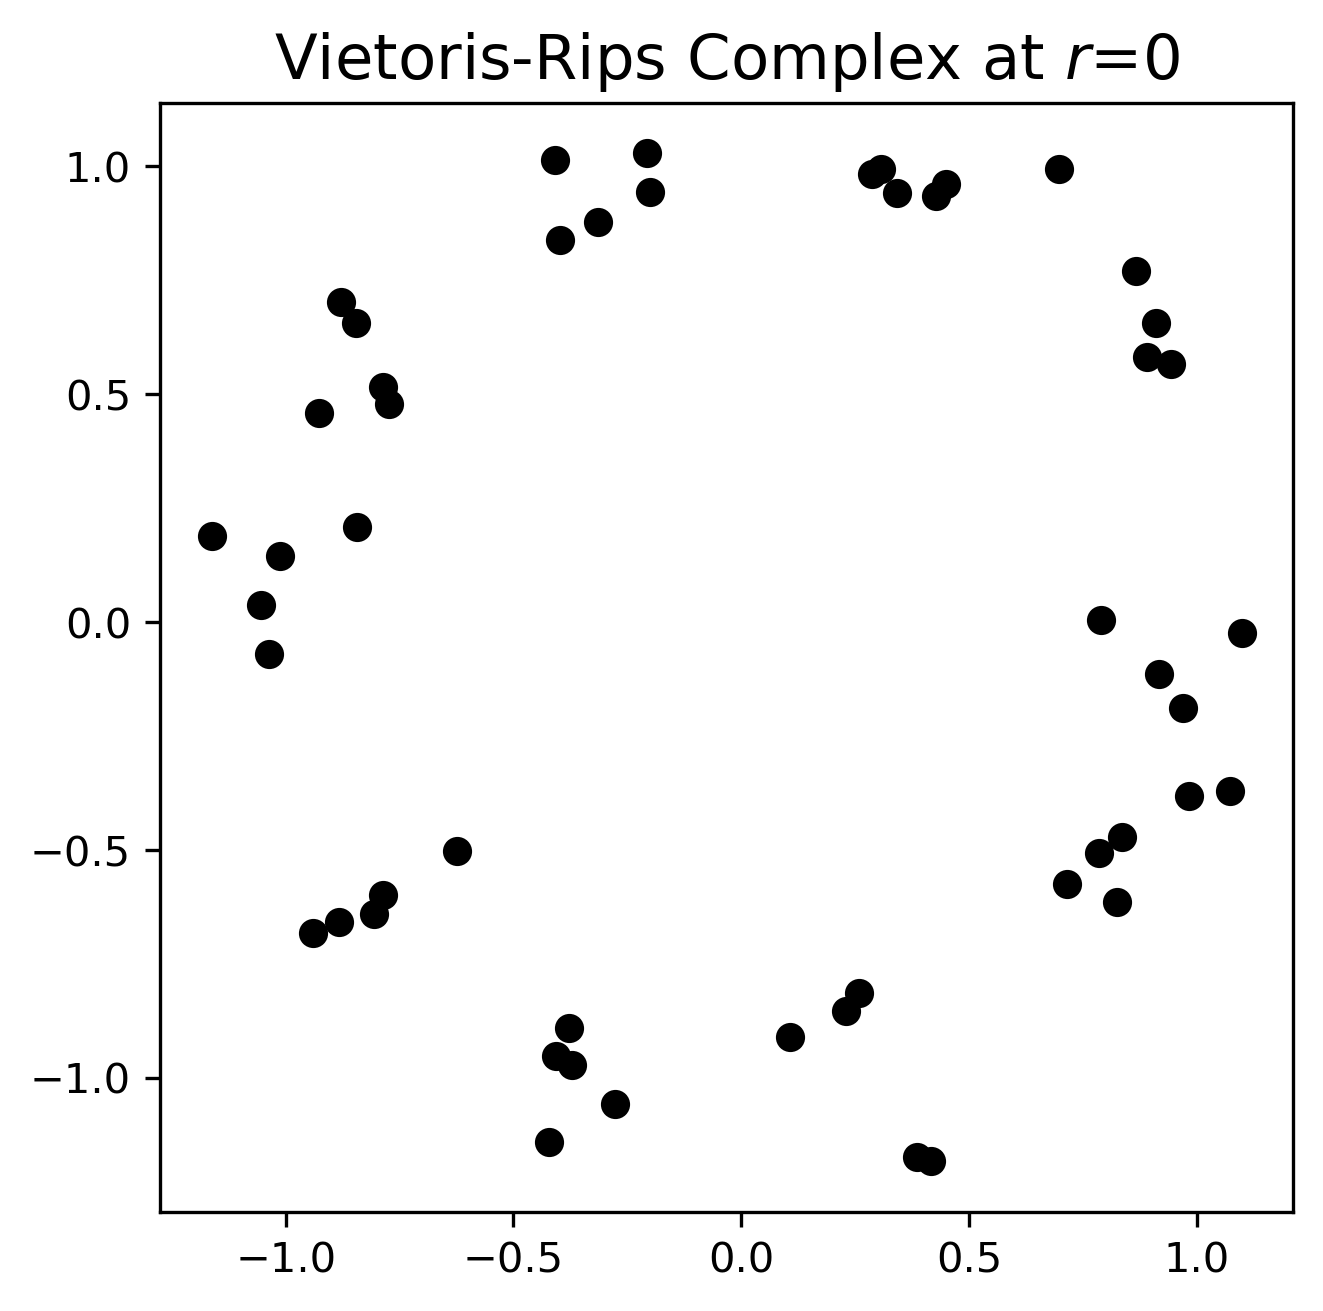
\includegraphics[width=\textwidth]{point_cloud_plot_r0.png}
    \end{subfigure}
    \hfill
    \begin{subfigure}[b]{0.22\textwidth}
        \centering
        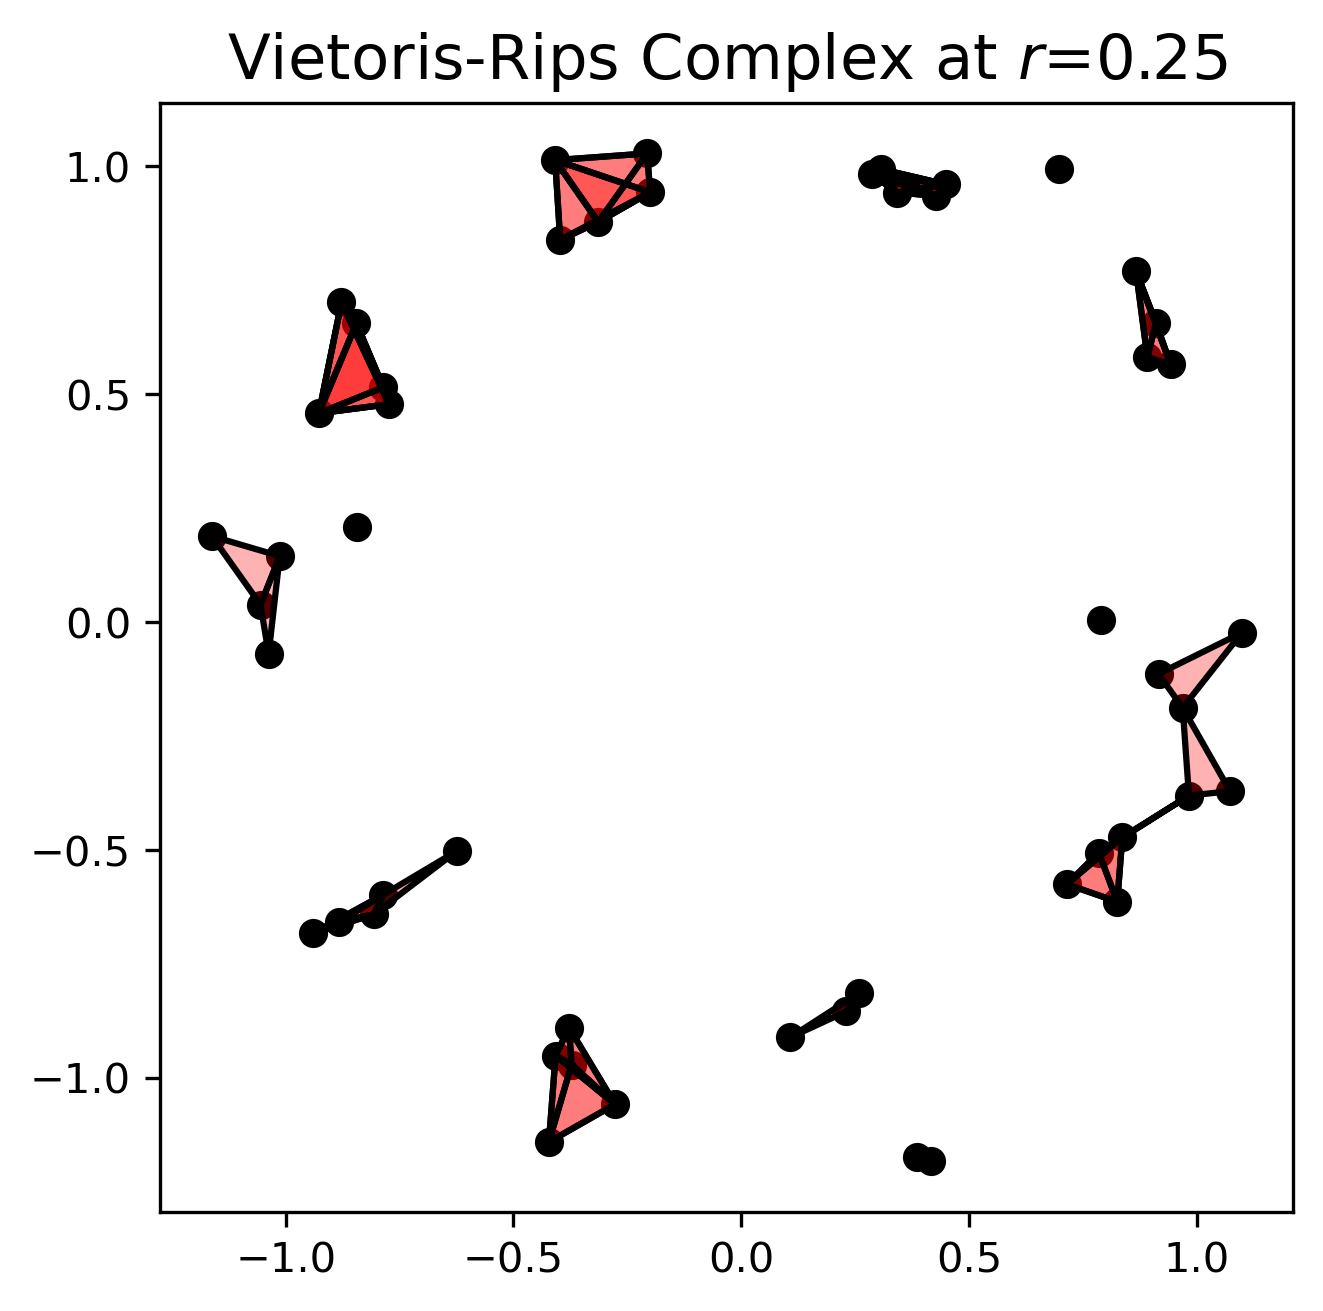
\includegraphics[width=\textwidth]{point_cloud_plot_r0_25.png}
    \end{subfigure}
        \hfill
    \begin{subfigure}[b]{0.22\textwidth}
        \centering
        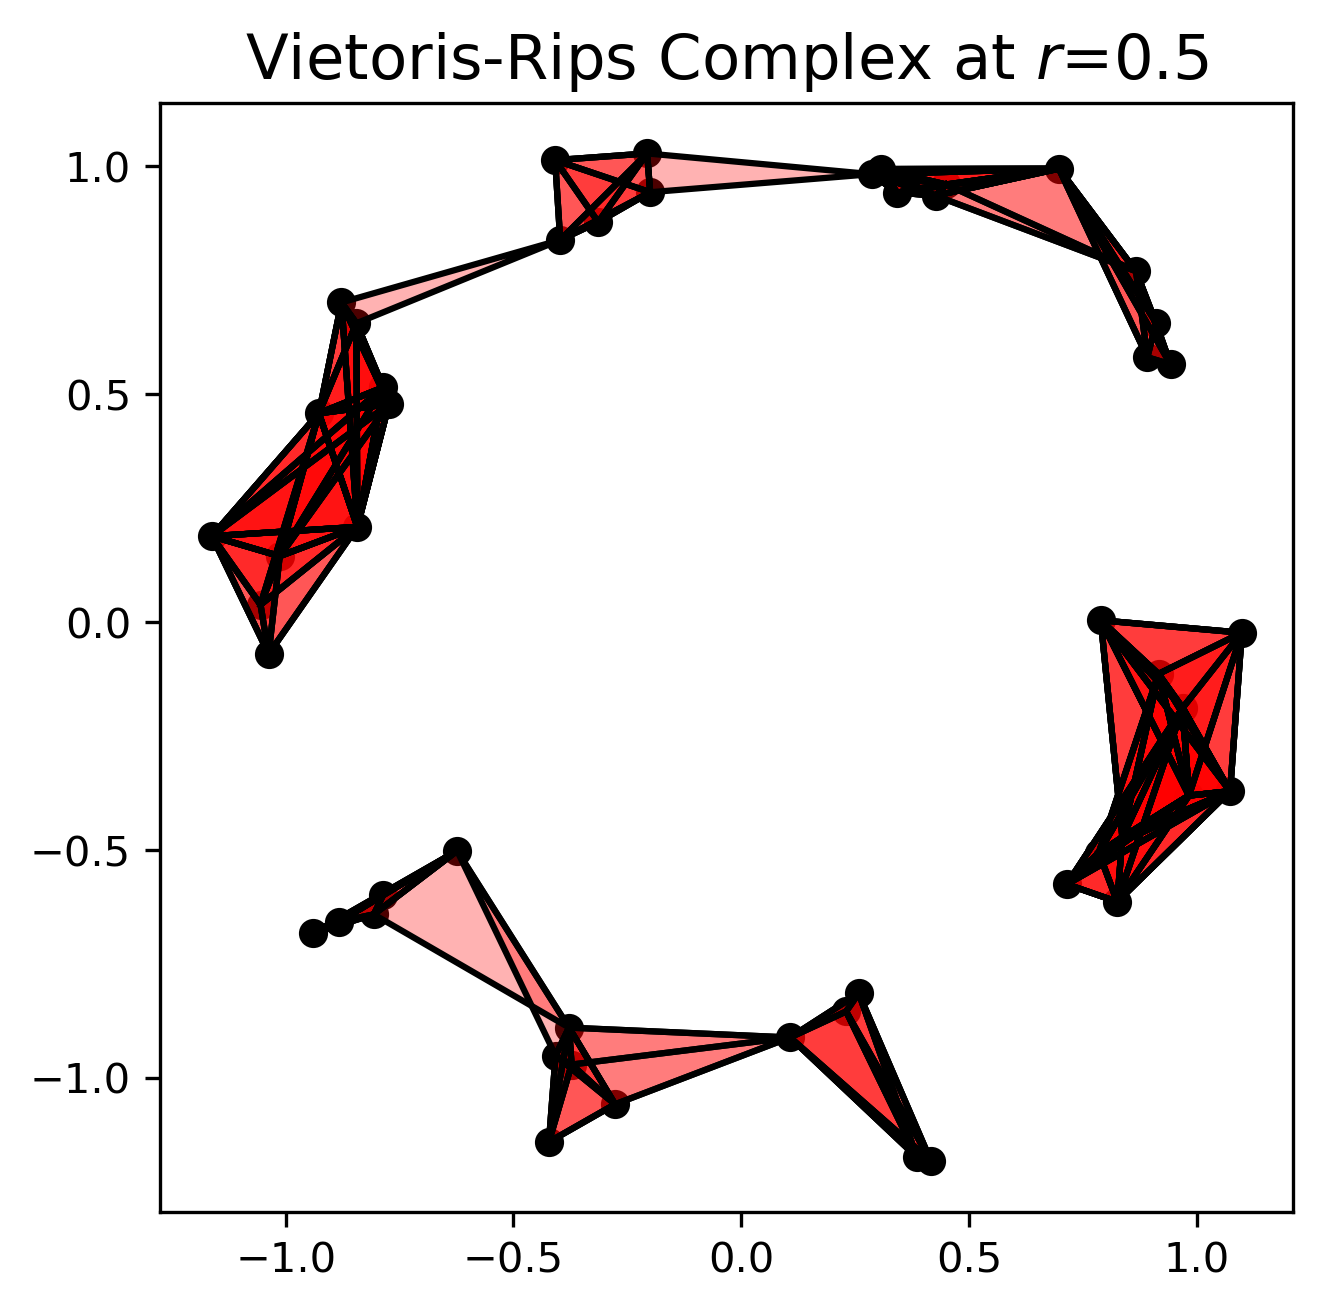
\includegraphics[width=\textwidth]{point_cloud_plot_r0_5.png}
    \end{subfigure}
        \hfill
    \begin{subfigure}[b]{0.22\textwidth}
        \centering
        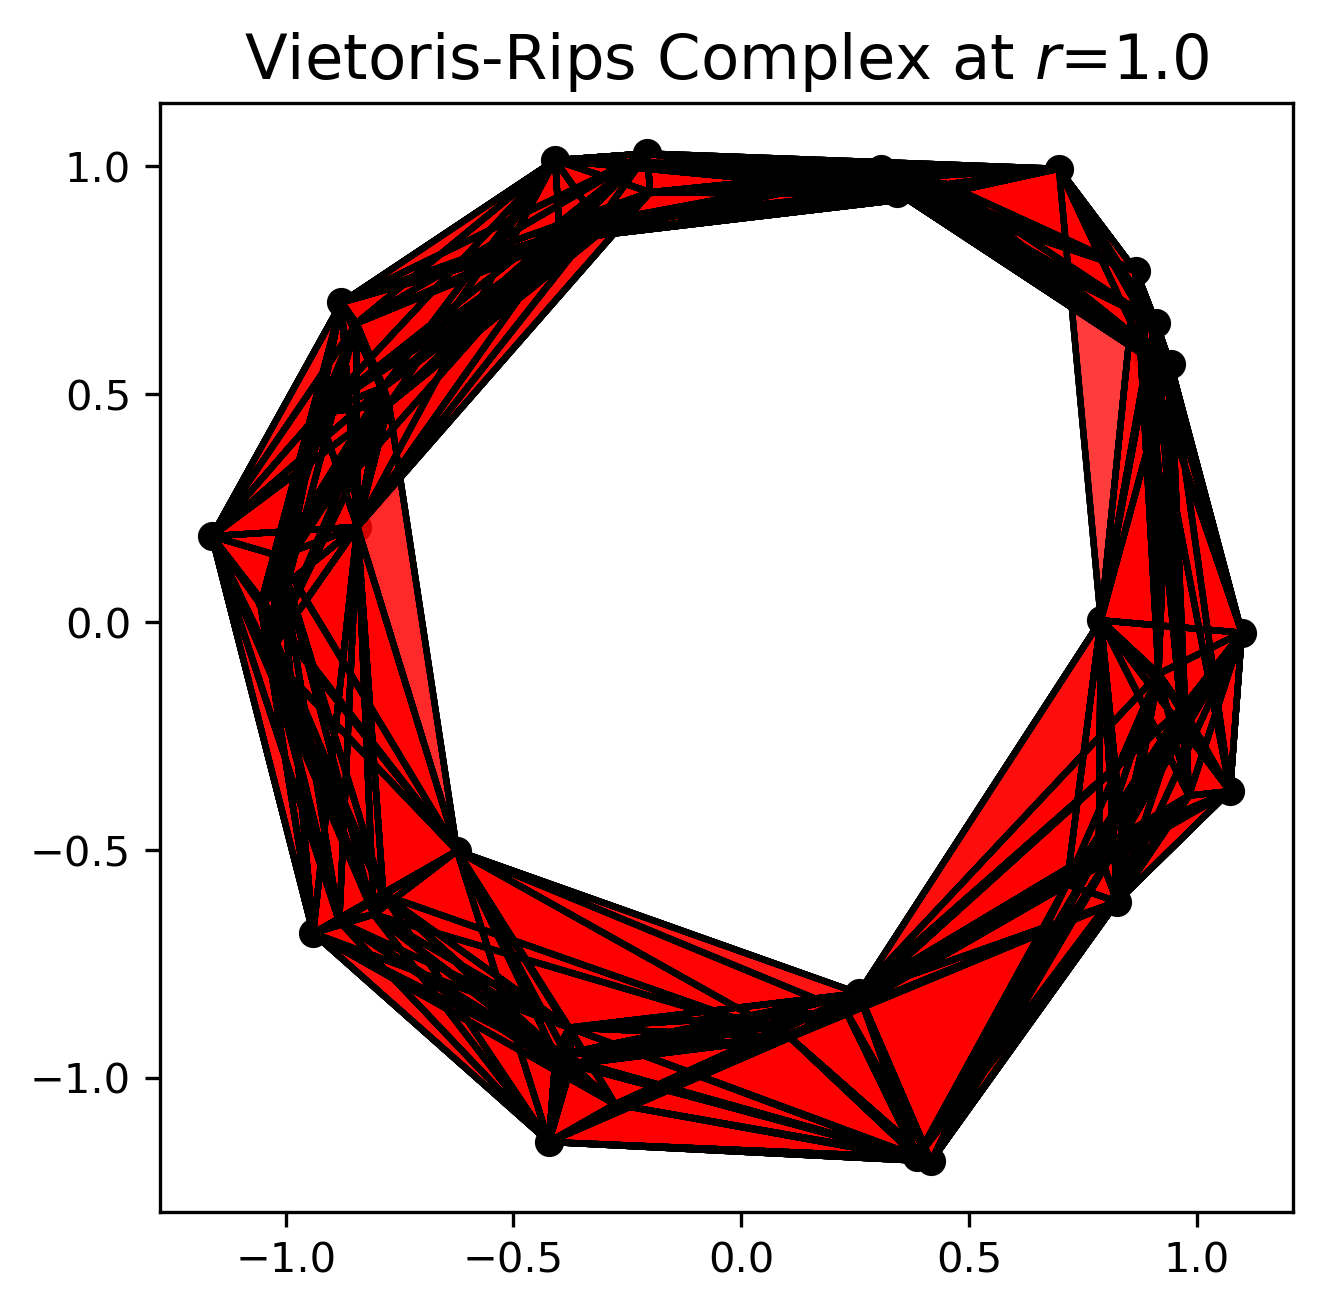
\includegraphics[width=\textwidth]{point_cloud_plot_r1_0.png}
    \end{subfigure}
    \caption{Vietoris-Rips complex of a point cloud as radius $r$ increases.}
    \label{fig:point_cloud_radii}
\end{figure}
\end{example}

\begin{example}[Persistence Diagram of a Vietoris-Rips Complex of a Point Cloud]
This example uses a randomly generated point cloud to create a persistence diagram from a Vietoris-Rips complex. When $r=0.5$, the persistence diagram shows three points at $d=\infty$ for $H_0$. This corresponds to the three connected components in the filtered simplicial complex. The points below infinity on the $y$-axis show the death times of points as they get added to one of the three connected components. Notice how there are only points on the $y$-axis: as Figure \ref{fig:point_cloud_radii} shows, all points are present when $r=0$, this means each point in the complex has a birth time of $0$.
\begin{figure}[H]
    \centering
    \begin{subfigure}[b]{0.45\textwidth}
        \centering
        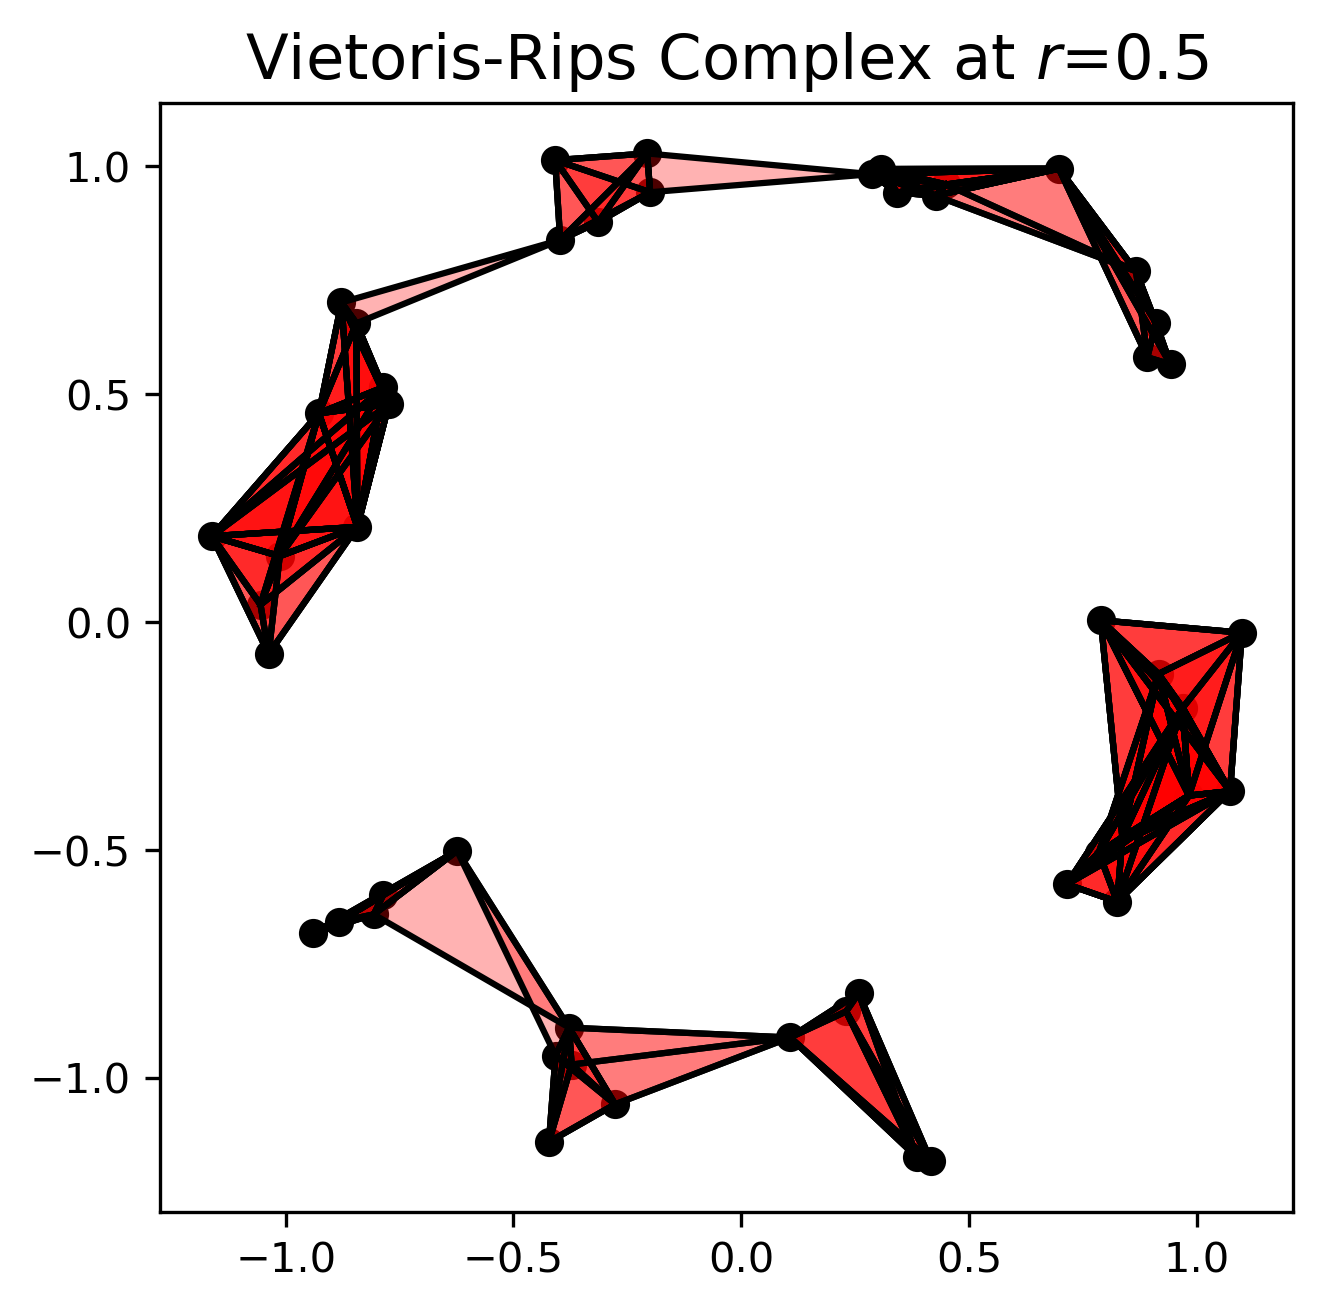
\includegraphics[width=\textwidth]{point_cloud_plot_r0_5.png}
    \end{subfigure}
    \hfill
    \begin{subfigure}[b]{0.45\textwidth}
        \centering
        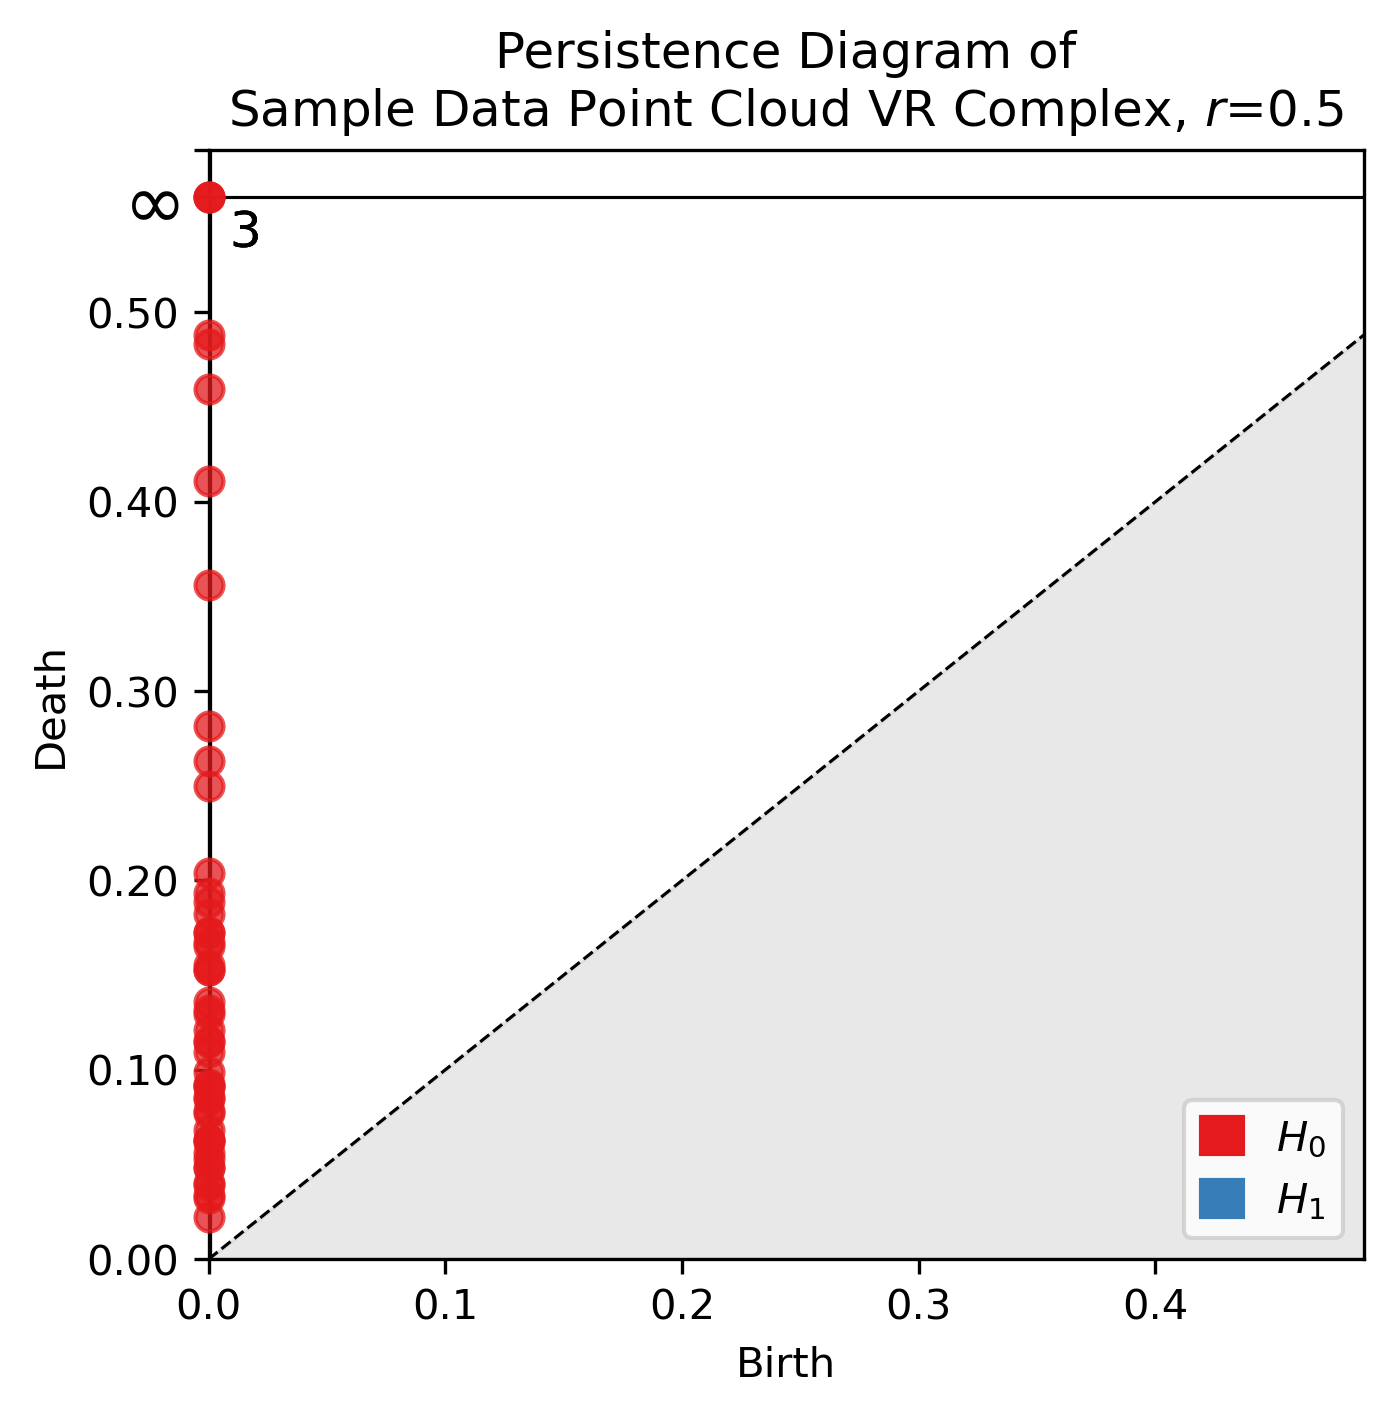
\includegraphics[width=\textwidth]{point_cloud_persdia_vr_0_5.png}
    \end{subfigure}
    \caption{Plot of a point cloud and persistence diagram of its Vietoris-Rips complex.}
    \label{fig:point_cloud_persdia}
\end{figure}
\end{example}

\newpage
\par The Čech and Vietoris-Rips complexes can be very computationally expensive, so an alternative filtered simplicial complex, the Alpha Complex, will need to be applied to the STL file data. Before we can define the Alpha Complex, we need to define an essential component of it, the Delaunay Triangulation.

\begin{definition}[Delaunay] We say a $k$-simplex whose vertices are in a set of points, $V$ is \textit{Delaunay} if there exists a circumsphere in that $k$-simplex such that no vertex of $V$ lies inside it \cite{tetgen}.
\end{definition}

\begin{definition}[Delaunay Triangulation] A \textit{Delaunay triangulation} is a unique triangulation on a vector space which is formed by creating a connection between points whenever their Voronoi cells (Def \ref{def:voronoi}) intersect such that all simplices in the space are Delaunay. This triangulation is the dual of its Voronoi cells \cite{deltri}\cite{tetgen}.
\end{definition}
\begin{figure}[H]
    \centering
    \begin{subfigure}[b]{0.35\textwidth}
        \centering
        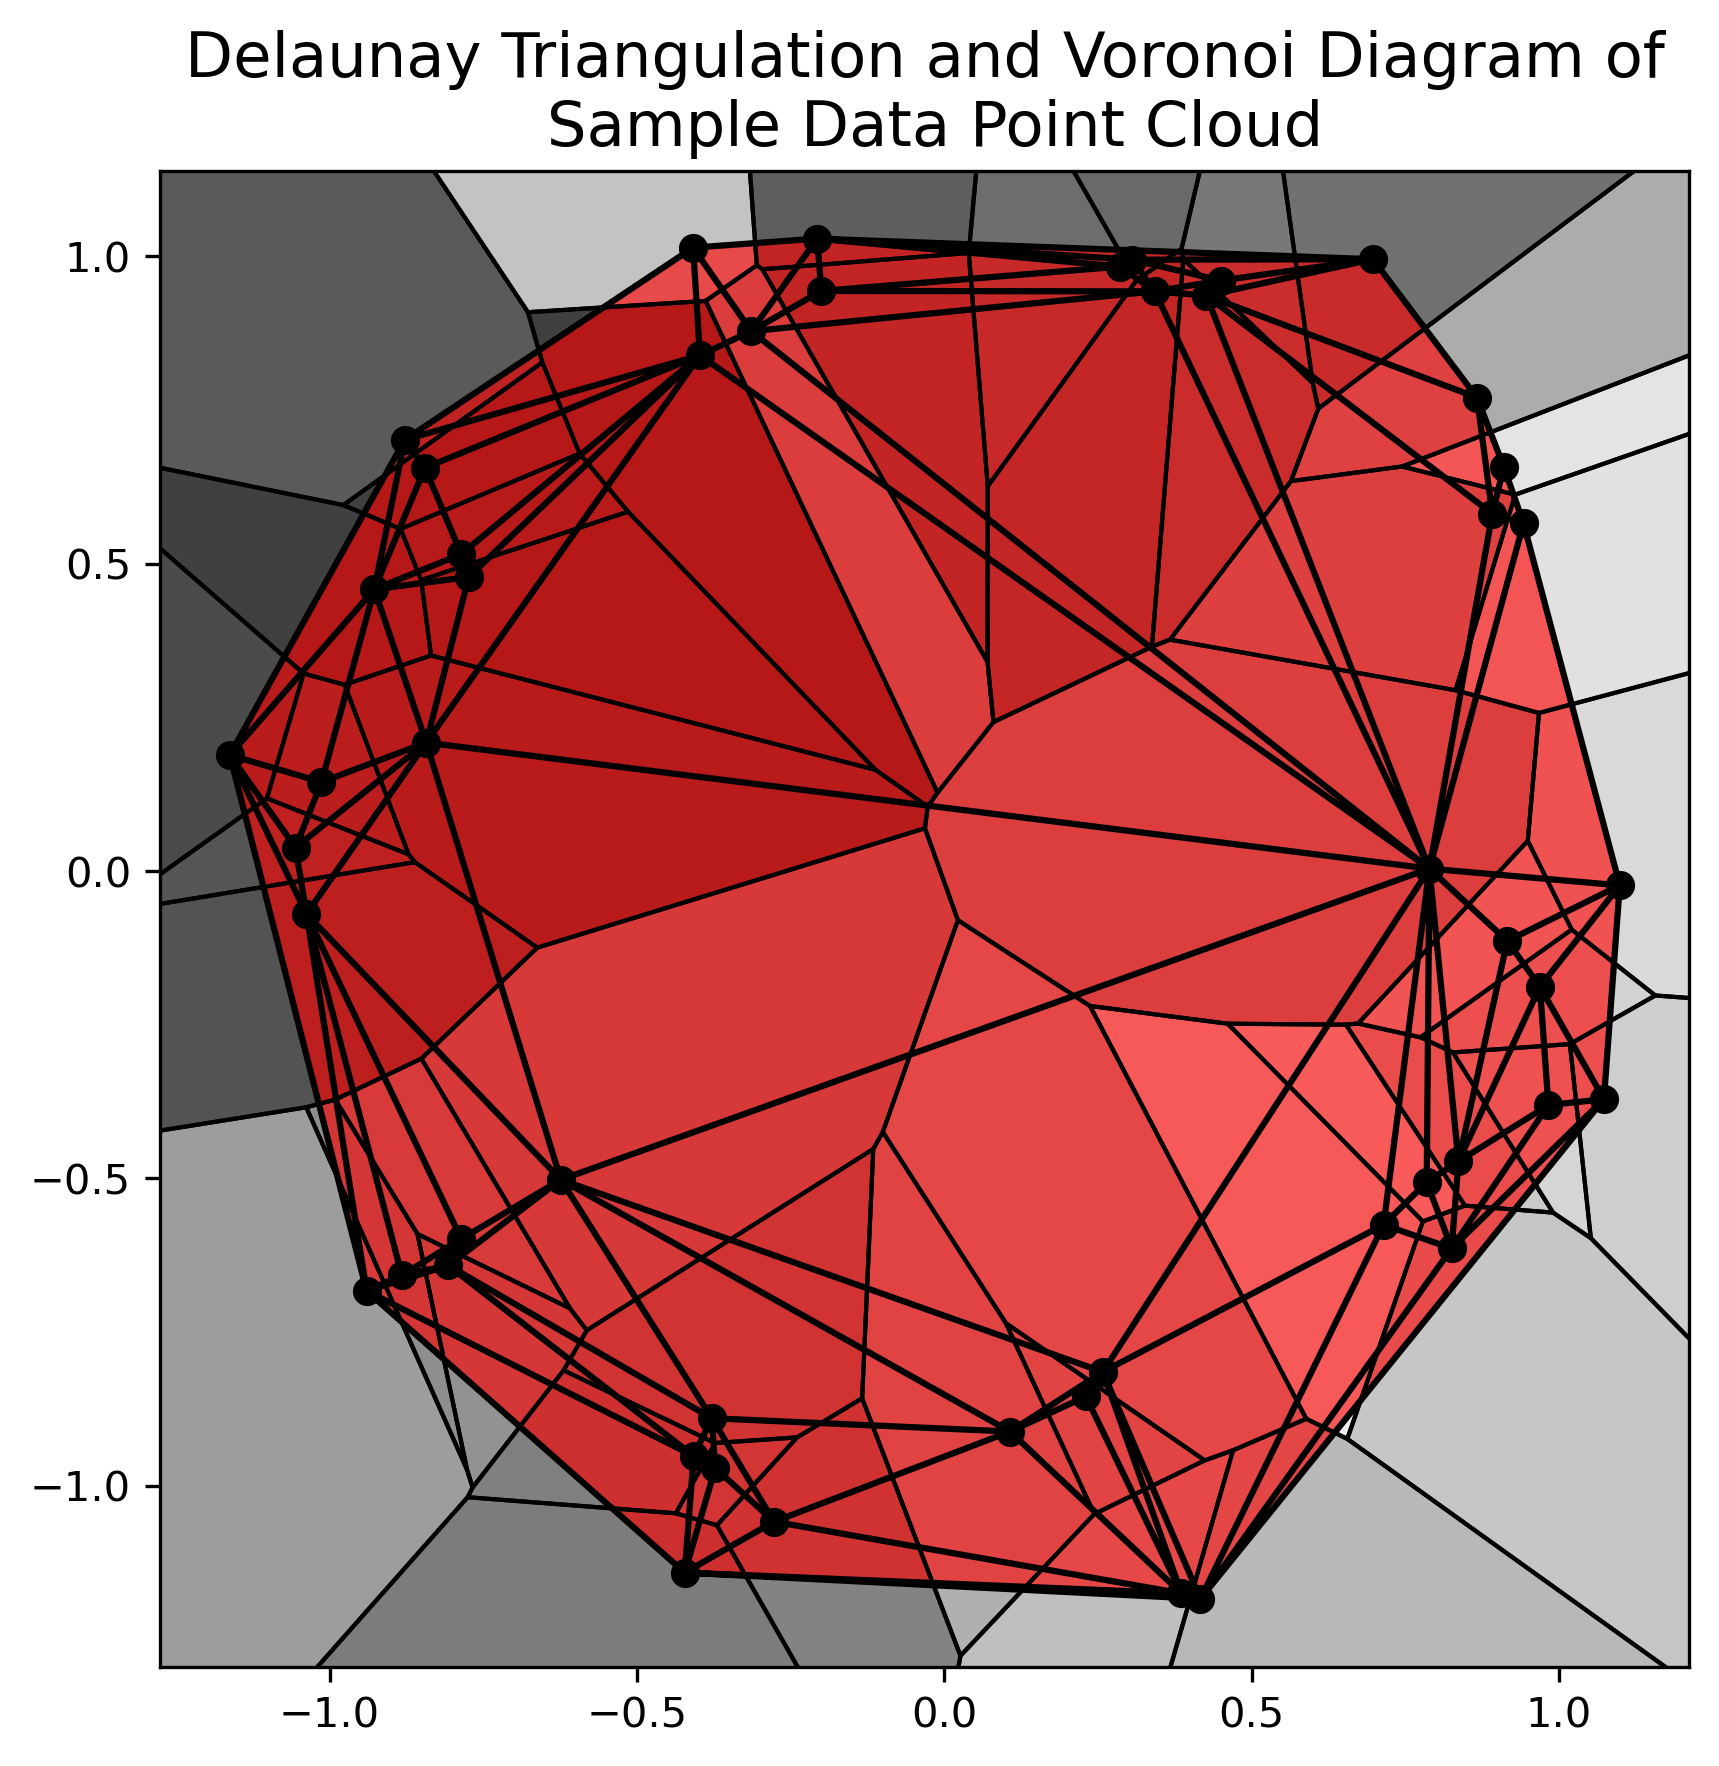
\includegraphics[width=\textwidth]{point_cloud_plot_del.png}
    \end{subfigure}
    \caption{Plot of a Delaunay Complex and Voronoi Cells applied to a point cloud.}
    \label{fig:point_cloud_del_voronoi}
\end{figure}

\begin{definition}[Gabriel]
When a mesh is created with a Delaunay Triangulation, certain edges in the triangulation can be considered \textit{Gabriel} when the open ball of the triangulated edge is empty of points \cite{gabriel}. However, not every edge in a triangulation needs to be considered Gabriel for it to be considered Delaunay. In $\mathbb{R}^{2}$, the figure below shows that every open ball, or circumcircle, of an edge contains no inner points.
\end{definition}
\begin{figure}[H]
    \centering
    \begin{subfigure}[b]{0.35\textwidth}
        \centering
        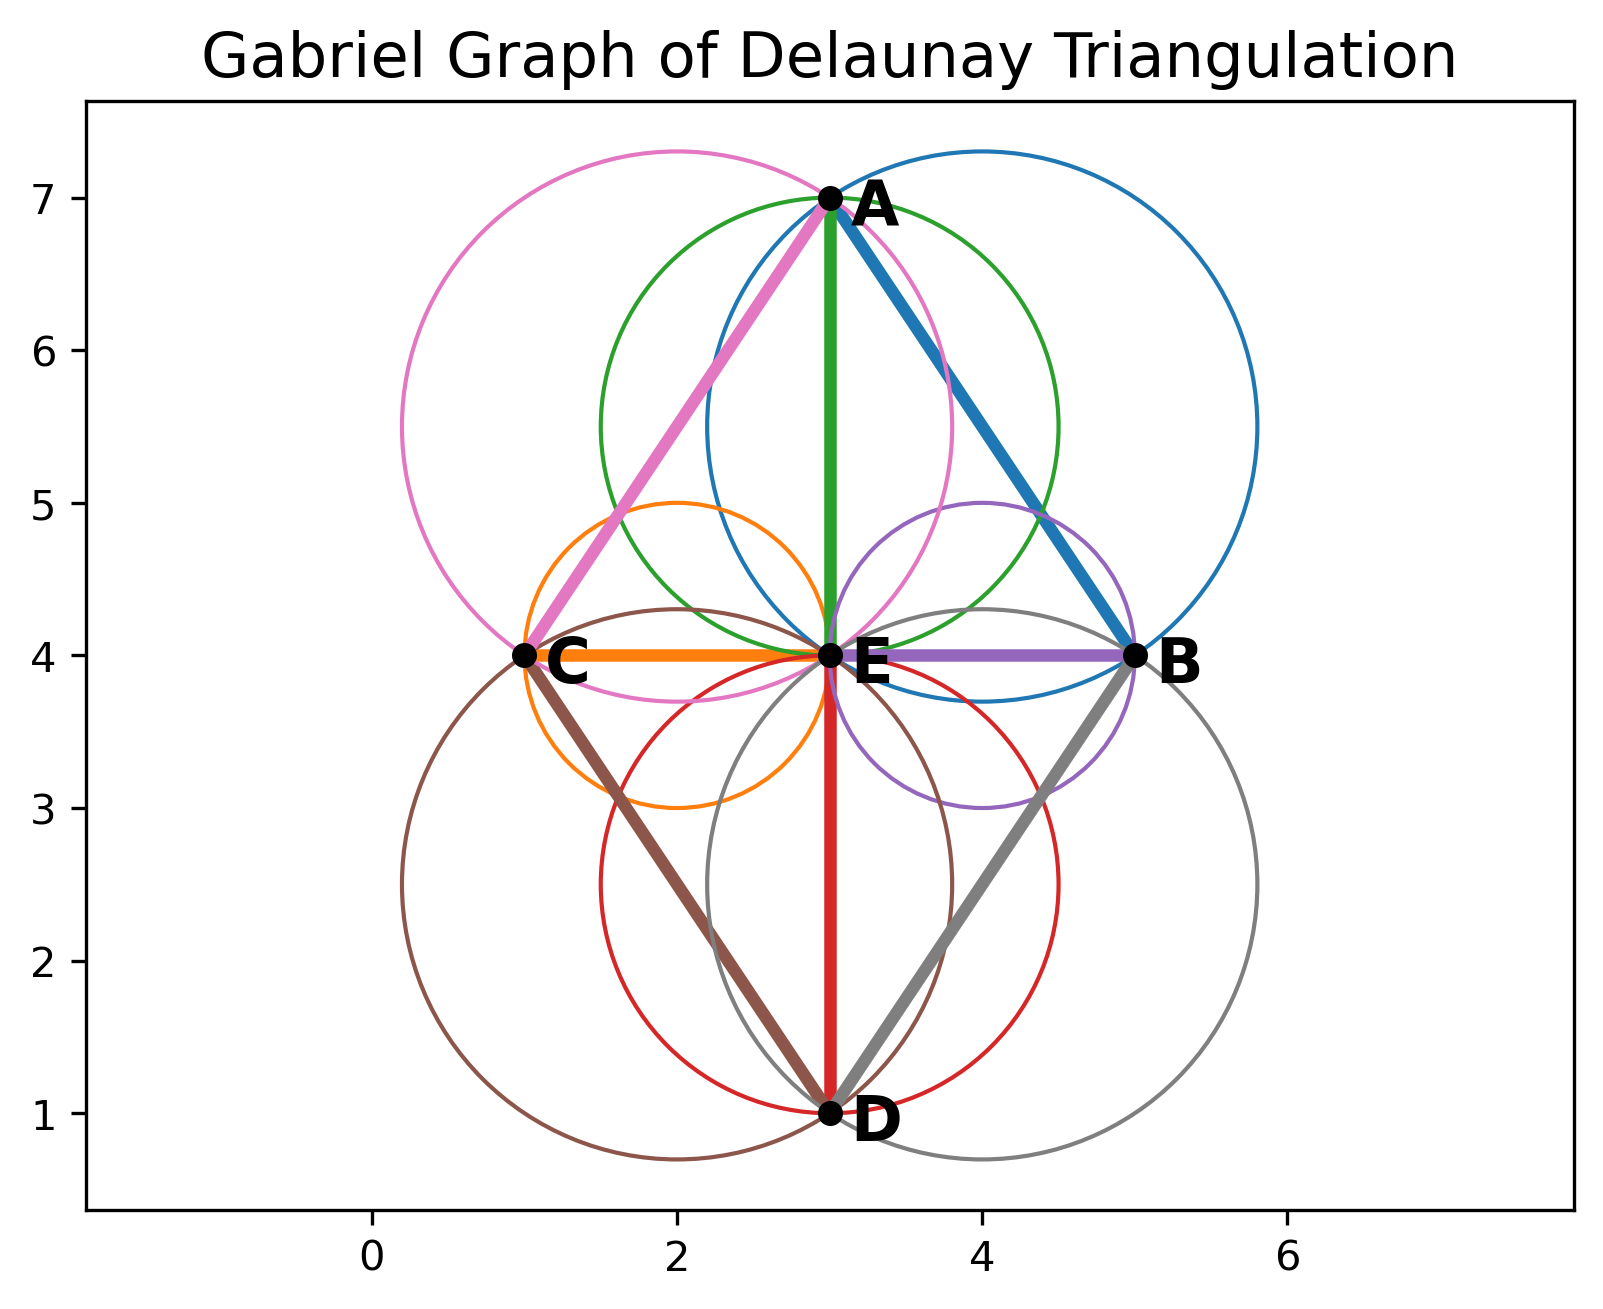
\includegraphics[width=\textwidth]{gabriel_circles.png}
    \end{subfigure}
        \begin{subfigure}[b]{0.35\textwidth}
        \centering
        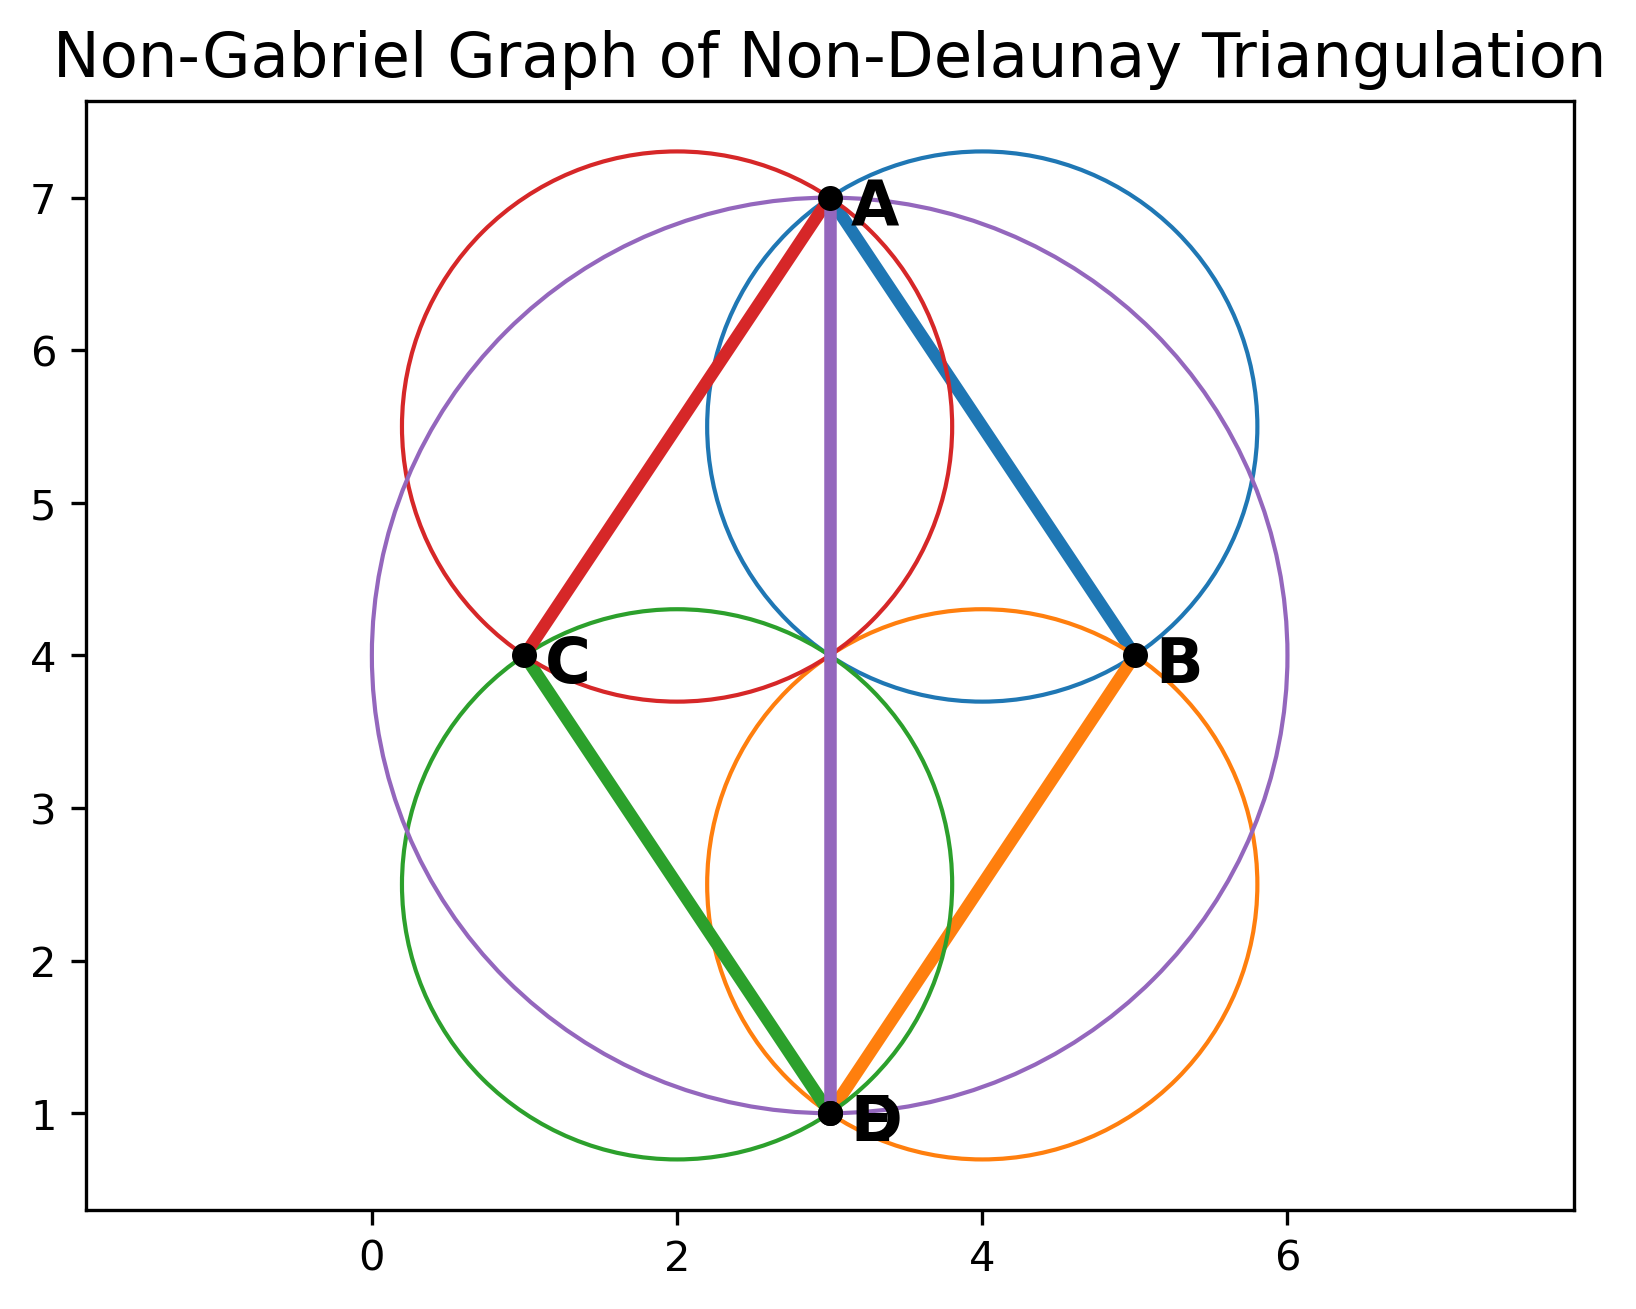
\includegraphics[width=\textwidth]{non_gabriel_circles.png}
    \end{subfigure}
    \caption{A Gabriel graph compared to a graph which cannot be Gabriel.}
    \label{fig:good_bad_gabriel}
\end{figure}

\begin{definition}[Alpha Complexes]
The Alpha complex (or $\alpha$-complex) exists within a finite metric space $(X, d)$ which is isometrically embedded in $\mathbb{R}^{m}$ (or another larger metric space, $(Y, d)$) with Euclidean distance. The alpha complex builds upon the Delaunay Triangulation with its use of Voronoi cells by introducing a radius parameter for an open metric ball. 
$$\alpha_{r}(X)=\{\sigma \subseteq X \mid \cap_{x\in \sigma} (B_{r}(X) \cap \mathsf{Vor}_{x}) \not= \emptyset\}$$
At $r=0$, the filtered simplicial complex consists only of the set of points in the metric space as individual connected components. As $r$ increases, the balls grow up to the boundary of or beyond their Voronoi cell. When two balls intersect, a connected component between those two points is formed. This continues until $r$ grows to create a simplex equivalent to the Delaunay triangulation.
\end{definition}

\par The Alpha complex is the ideal filtered simplicial complex to use when analyzing the homology of 3D objects as it can show us when connected components and holes are born and die in the persistent homology of the object while the growth of $r$ is self-contained to the maximum diameter of the object. The end growth point of the object's Delaunay triangulation also allows for the Alpha complex to be the least computationally expensive persistent homology method of the three we have defined.

\newpage
\begin{example}[Alpha Complex applied to a Point Cloud]\label{ex:point_cloud_alpha}
\par Fig \ref{fig:point_cloud_alpha_complex} shows an Alpha complex created with the python library \verb"Gudhi", which defines its growing radii parameter as $r^{2}$ to birth and death times. To understand events at certain radii, we denote plots with $r^{2}$ for birth and death times, and $r$ for Euclidean distance.
\par Two holes were created with birth times of $r^{2}=0.2308$ and $r^{2}=0.3068$. The first hole dies at $r^{2}=0.8045$. To understand why the second hole dies relatively quickly at $r^{2}=0.3069$, we can compare it to the filled-in triangle formed between $r^{2} = 0.23084$ and $r^{2} = 0.29$. The points of the triangle which make up the second hole have voronoi cells which intersect close to or exactly at the intersection point of all three voronoi cells. As one of the three balls grows slightly, the hole gets filled in $r^{2}=0.0001$ later. Three voronoi cells of points from the filled-in triangle all intersect at different times, creating the filled-in triangle instantly upon the third intersection.
\begin{figure}[H]
    \centering
    \begin{subfigure}[b]{0.26\textwidth}
        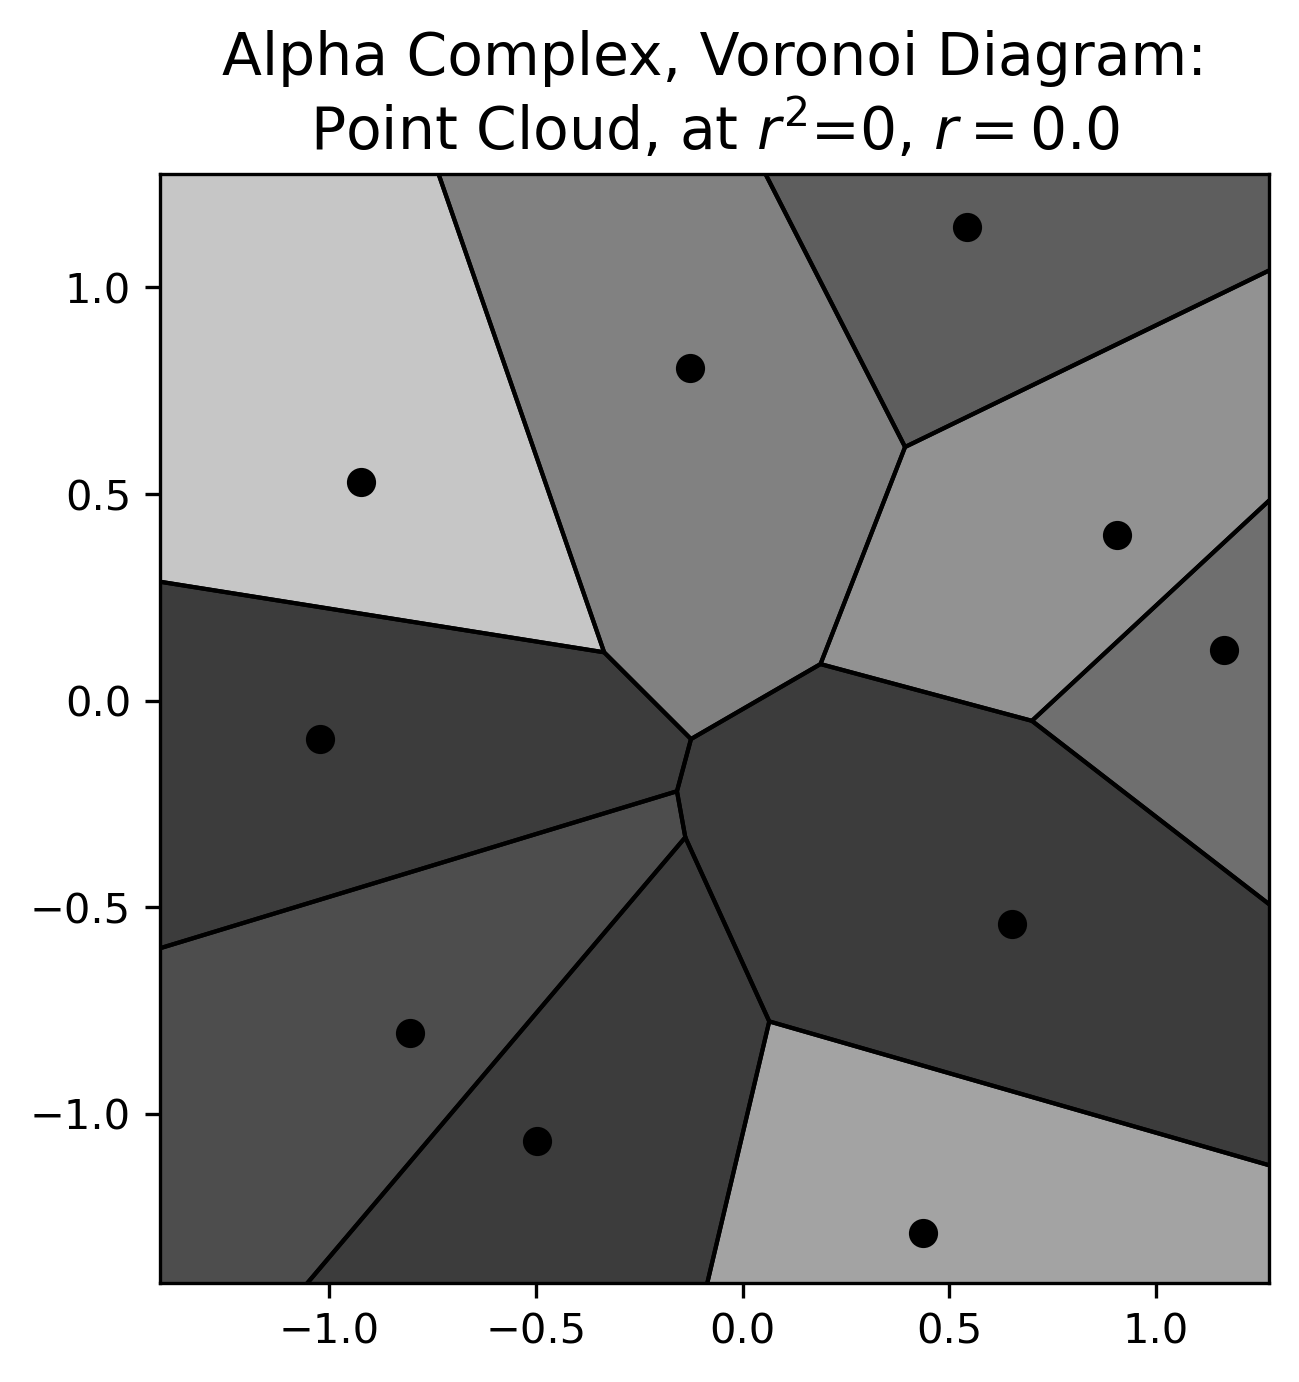
\includegraphics[width=\textwidth]{point_cloud_plot_alpha_0.png}
    \end{subfigure}
    \begin{subfigure}[b]{0.26\textwidth}
        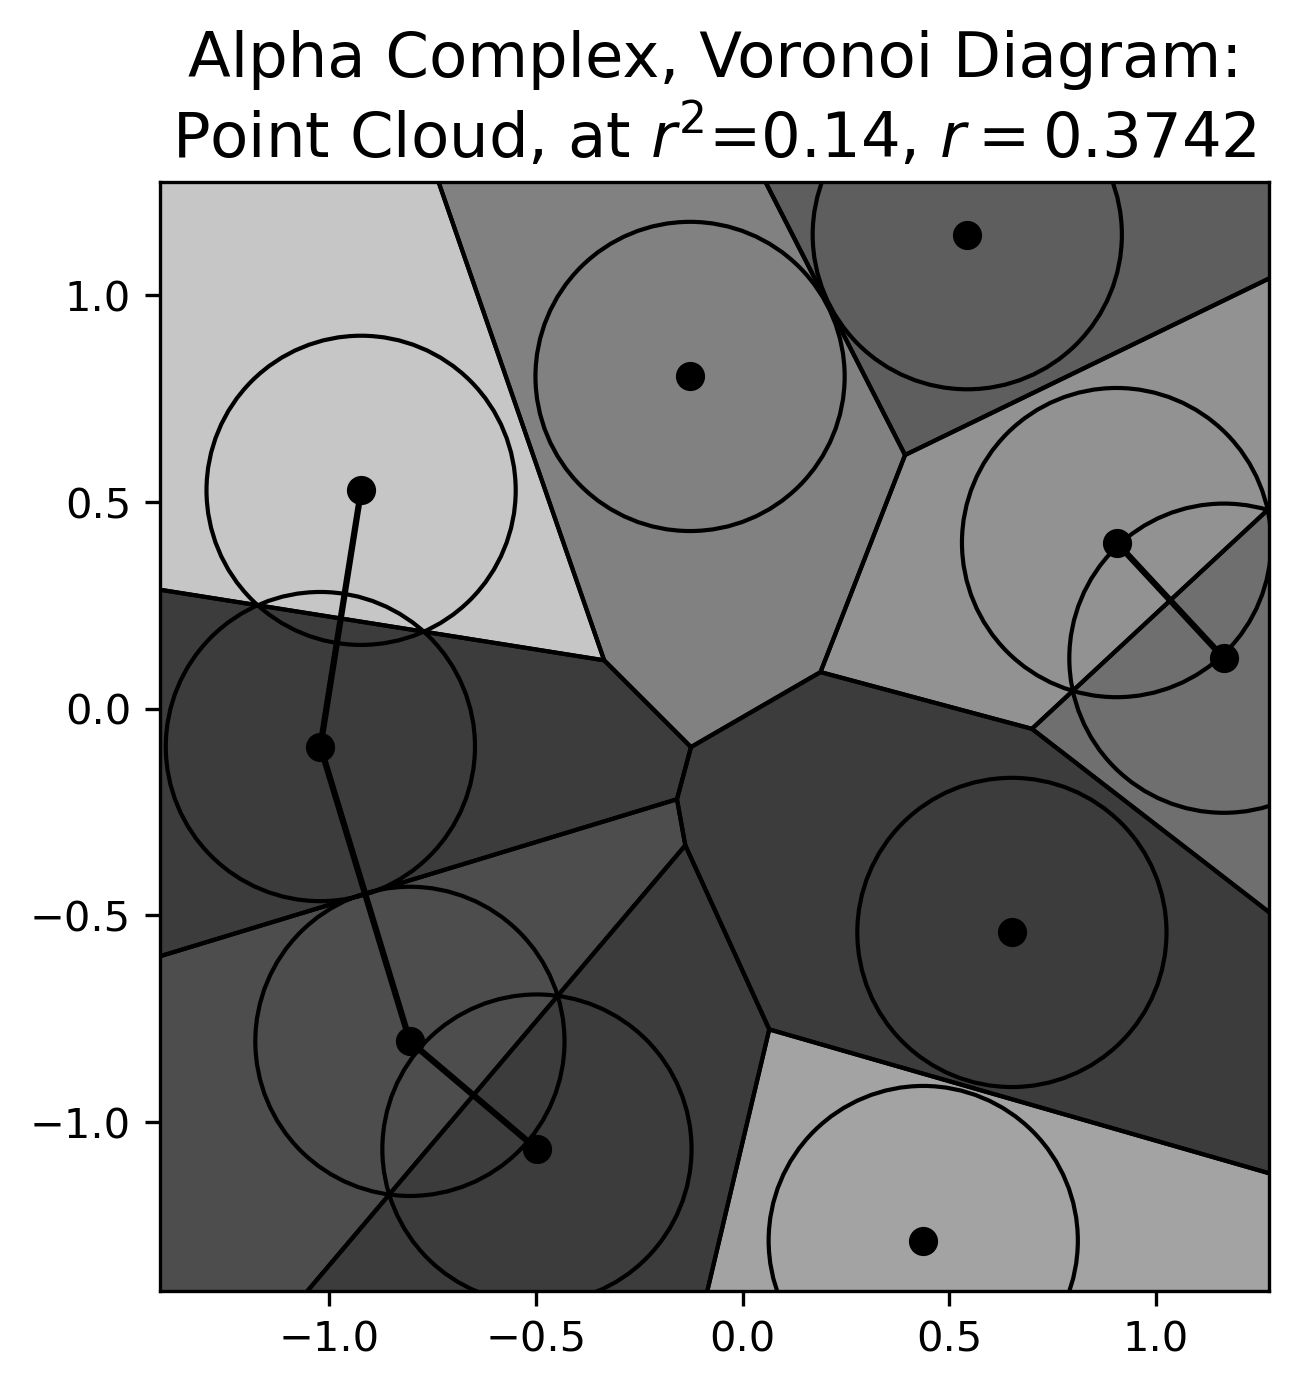
\includegraphics[width=\textwidth]{point_cloud_plot_alpha_1.png}
    \end{subfigure}
    \begin{subfigure}[b]{0.26\textwidth}
        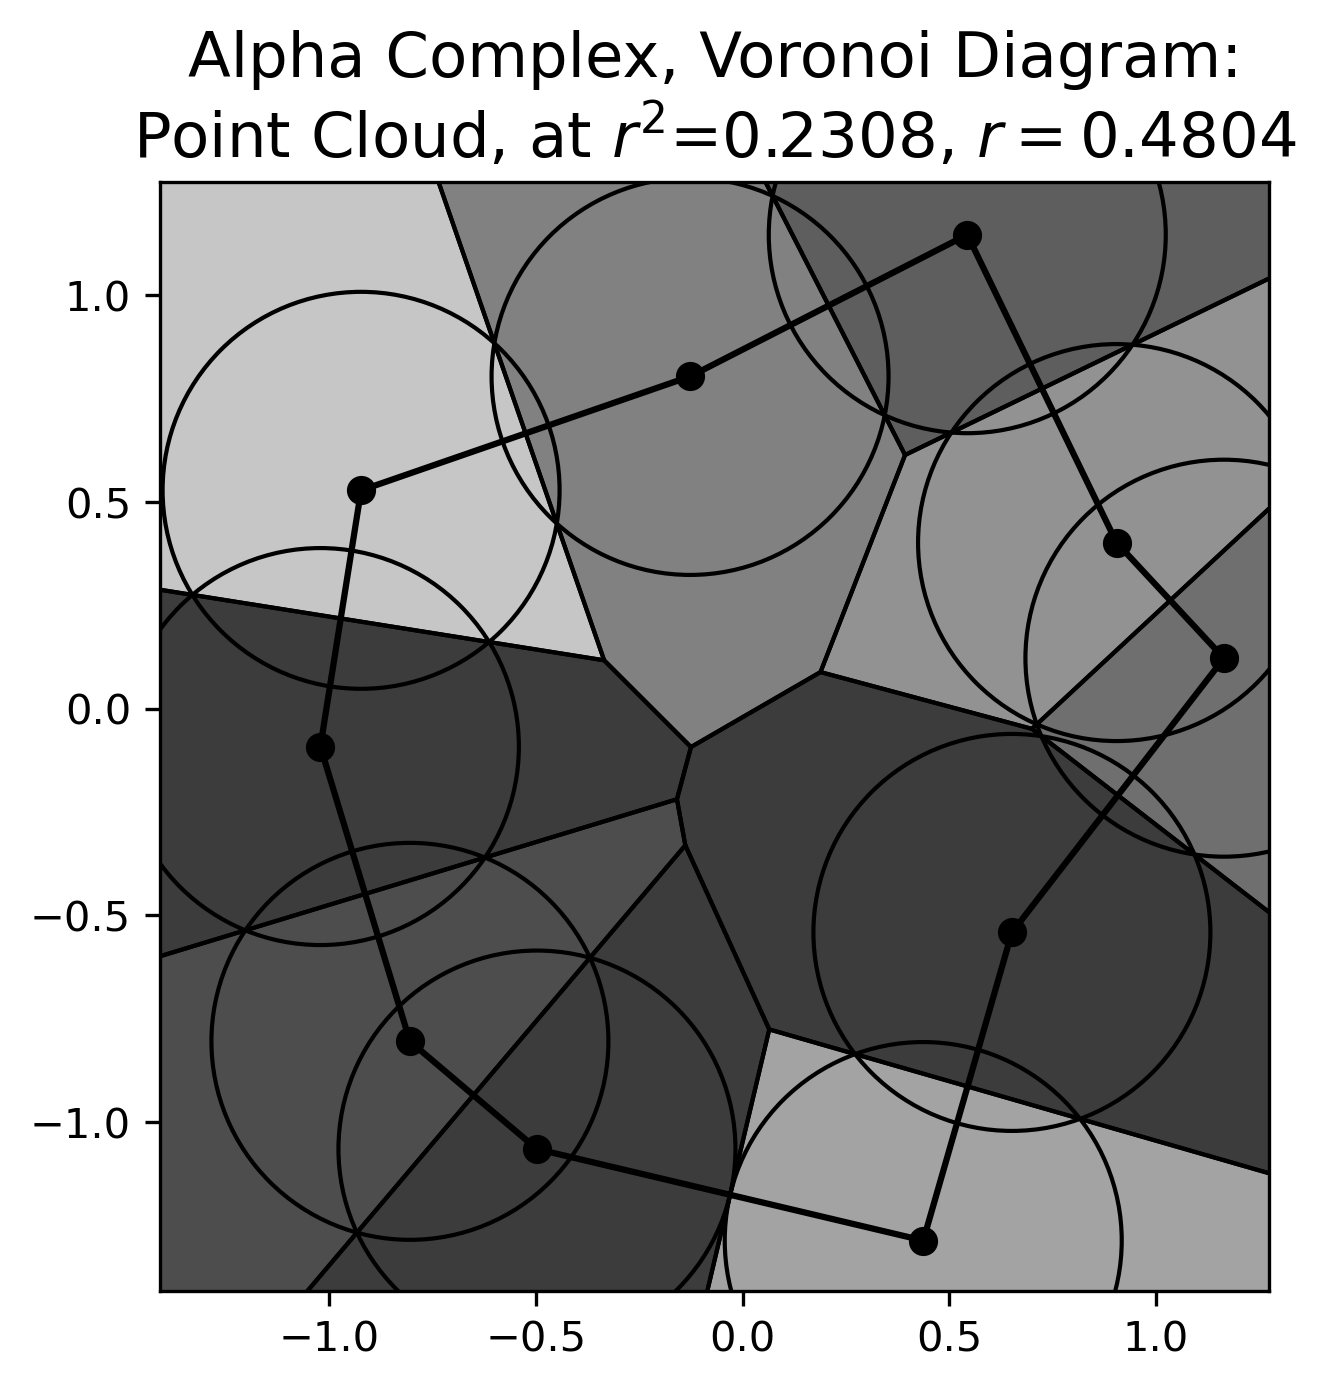
\includegraphics[width=\textwidth]{point_cloud_plot_alpha_2.png}
    \end{subfigure}
    \begin{subfigure}[b]{0.26\textwidth}
        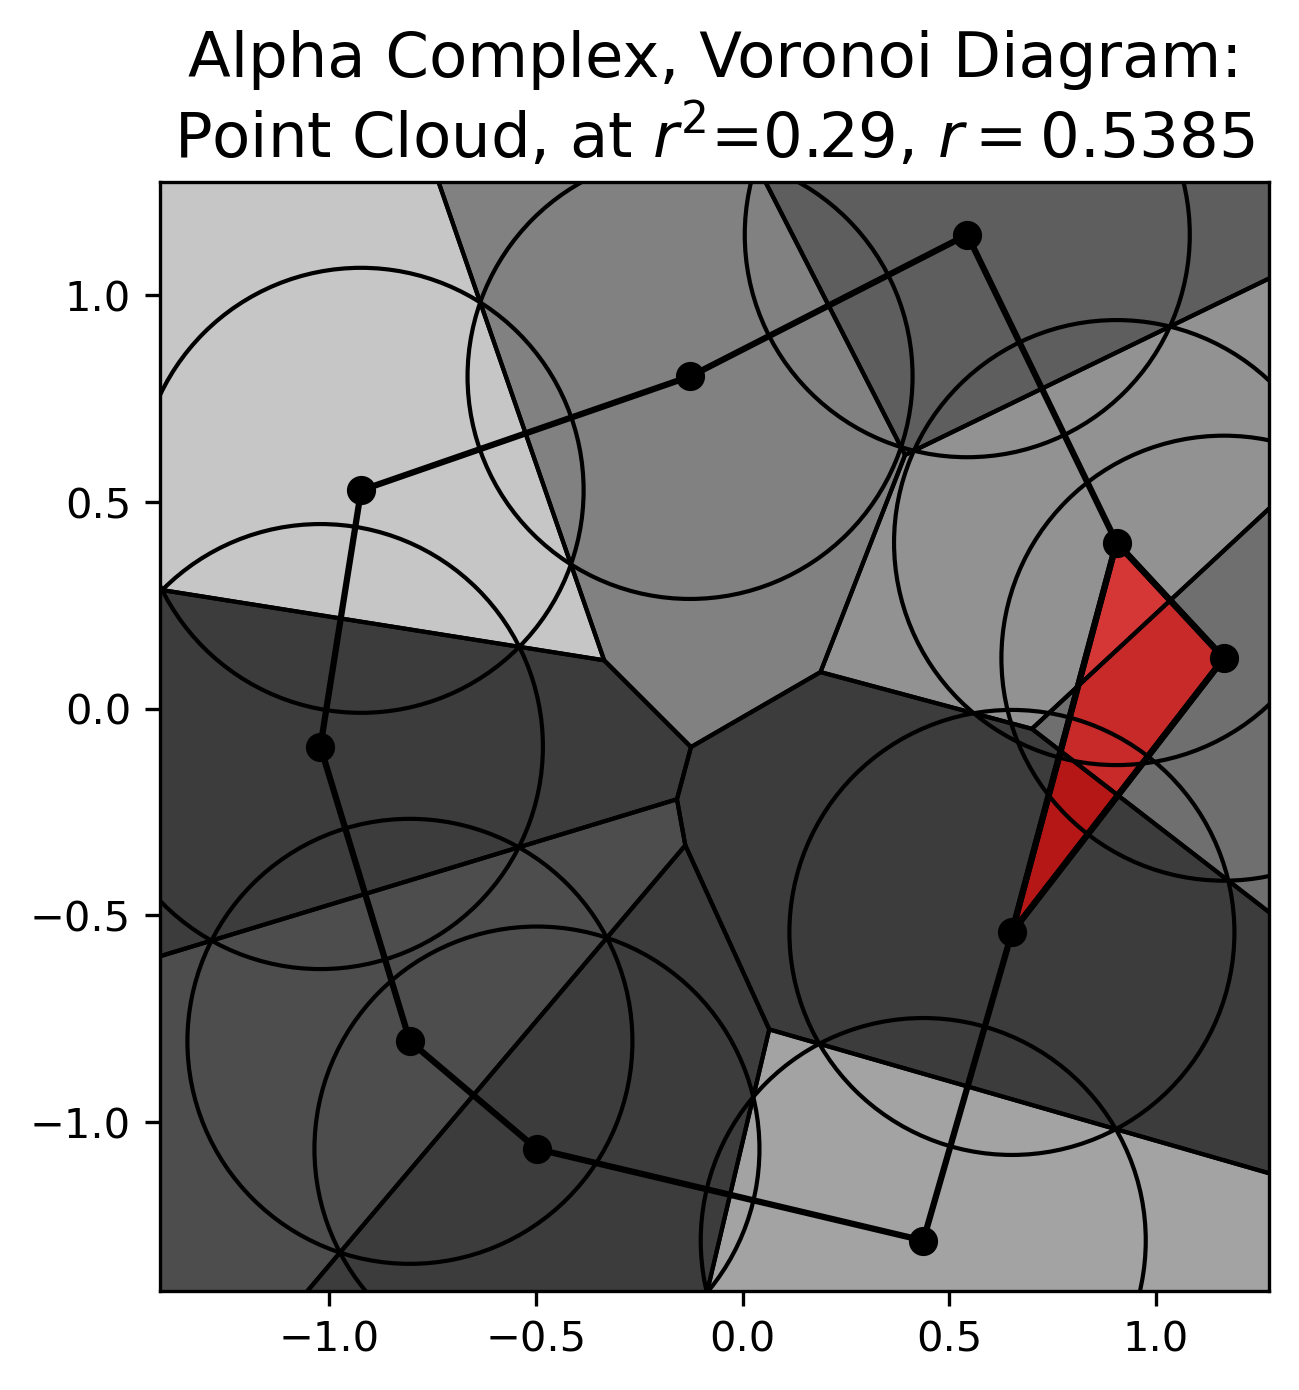
\includegraphics[width=\textwidth]{point_cloud_plot_alpha_3.png}
    \end{subfigure}
    \begin{subfigure}[b]{0.26\textwidth}
        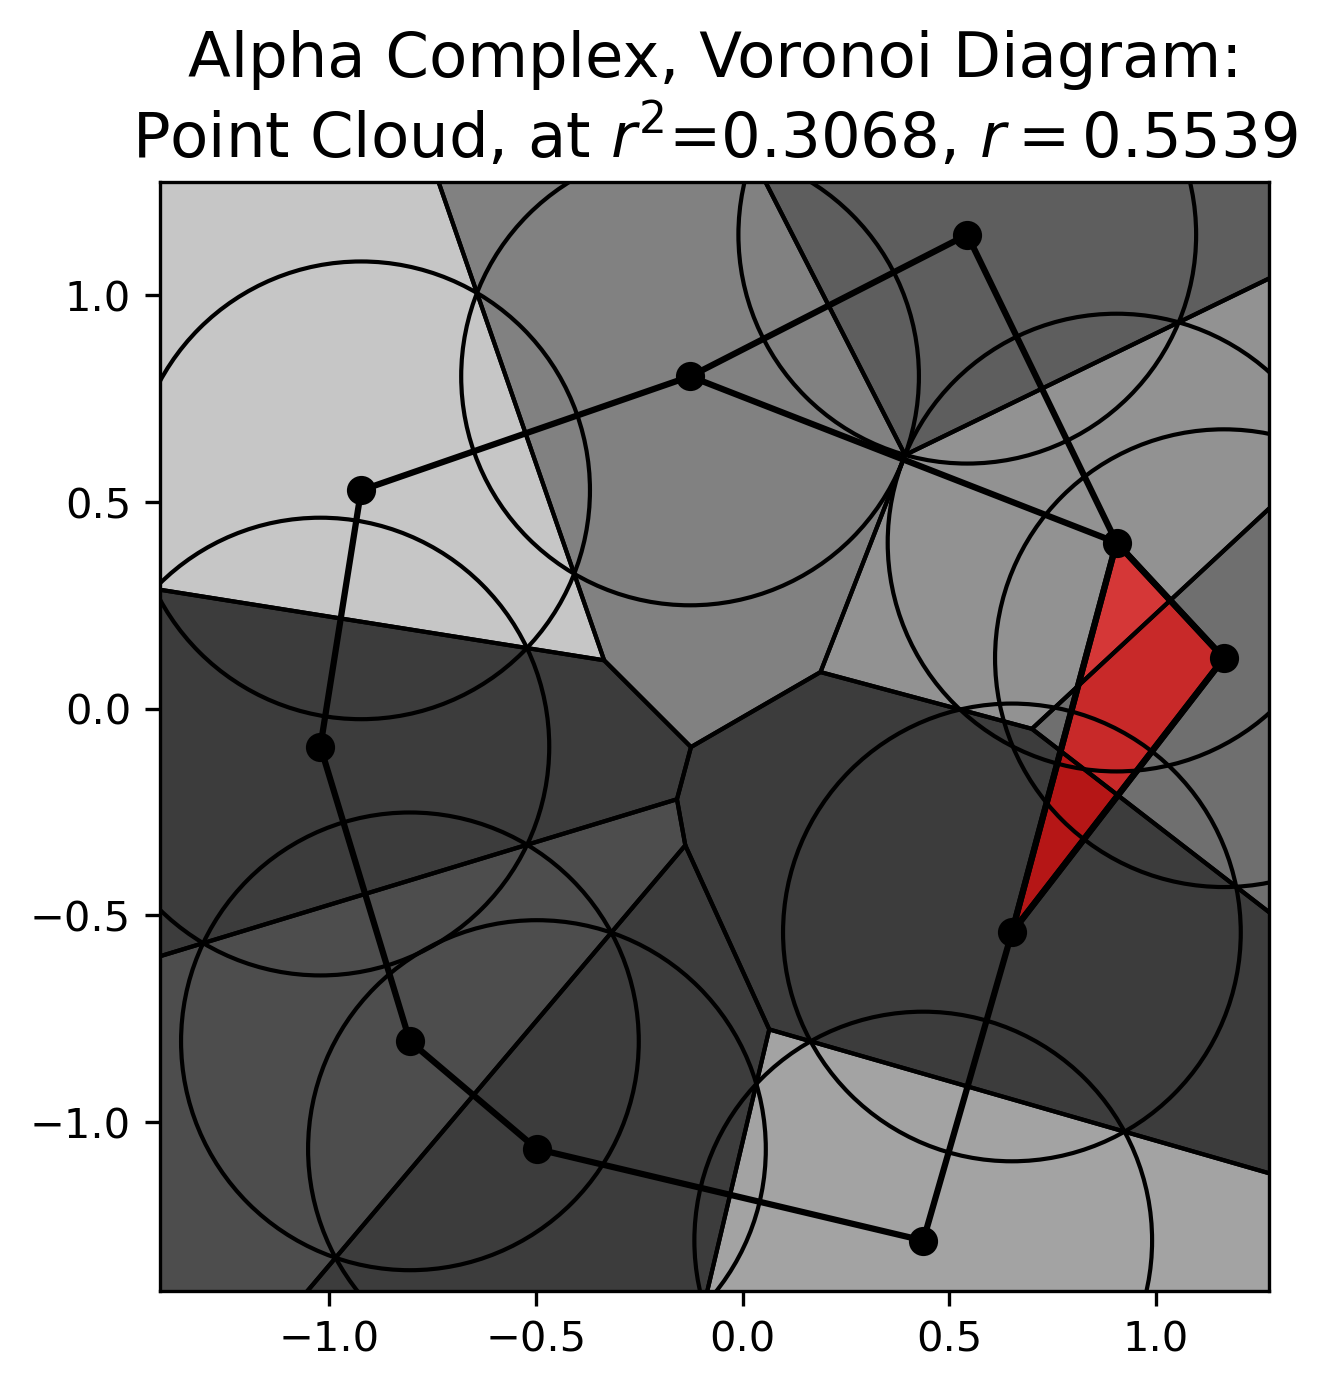
\includegraphics[width=\textwidth]{point_cloud_plot_alpha_4.png}
    \end{subfigure}
    \begin{subfigure}[b]{0.26\textwidth}
        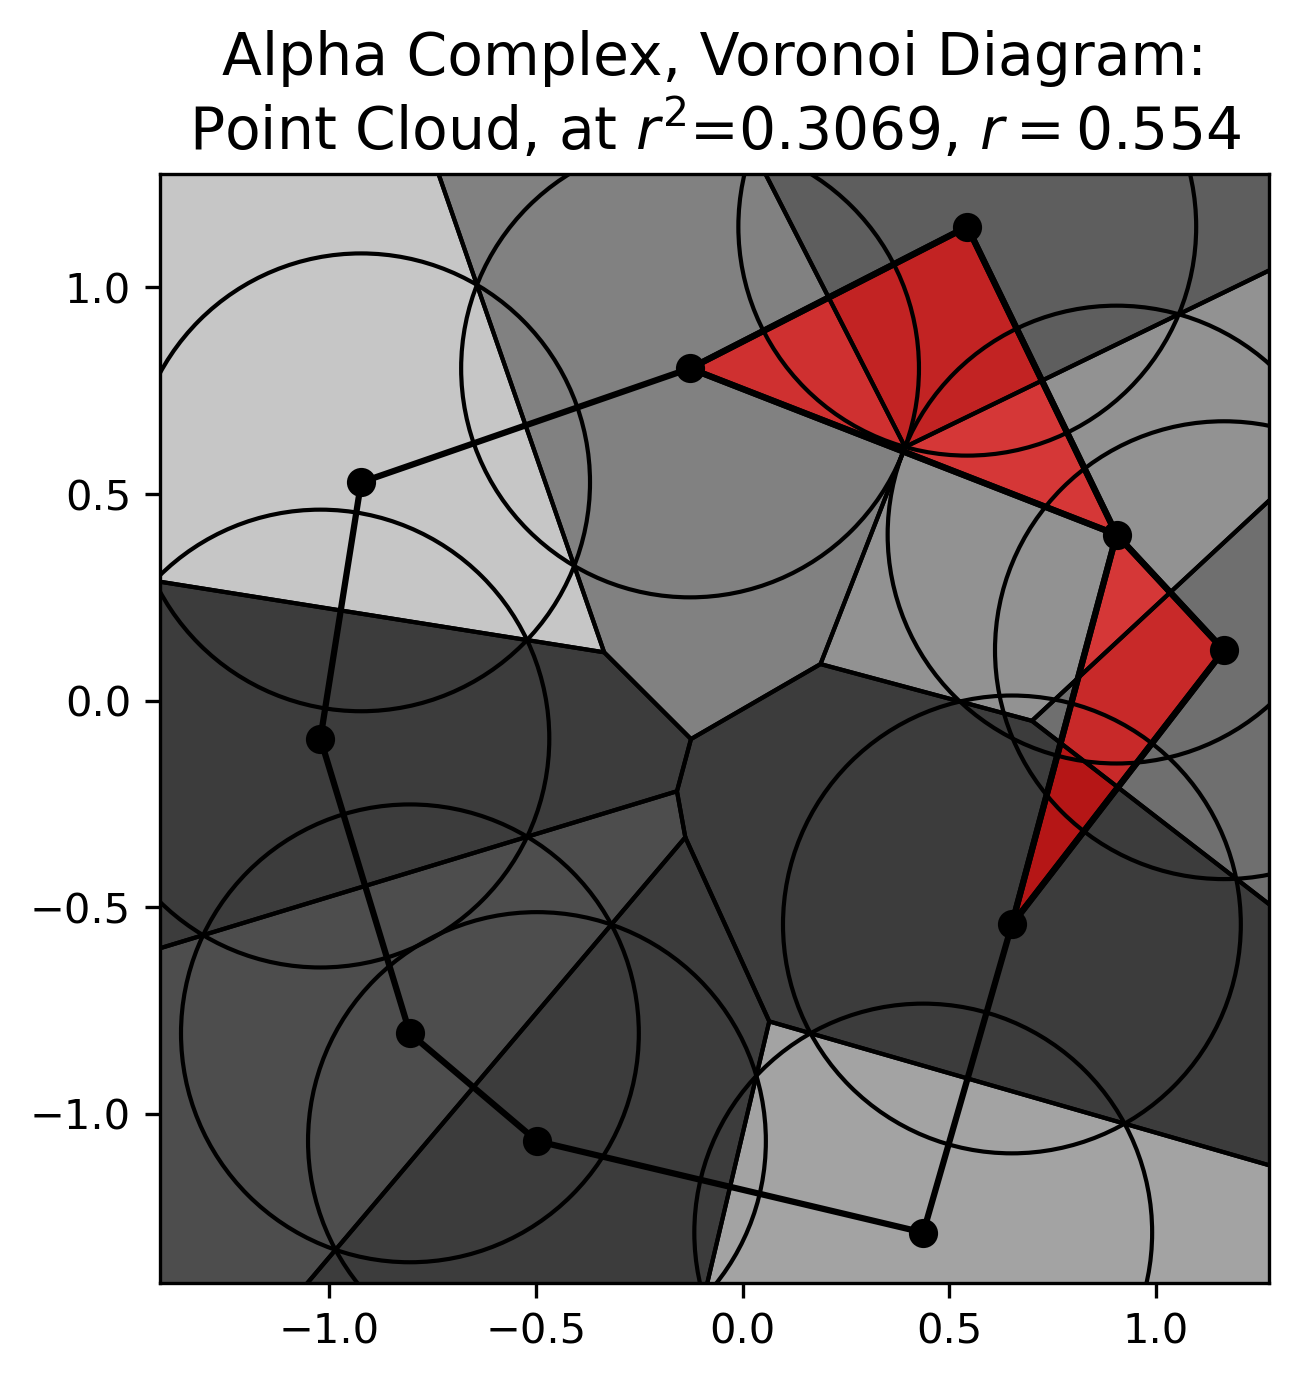
\includegraphics[width=\textwidth]{point_cloud_plot_alpha_5.png}
    \end{subfigure}
    \begin{subfigure}[b]{0.26\textwidth}
        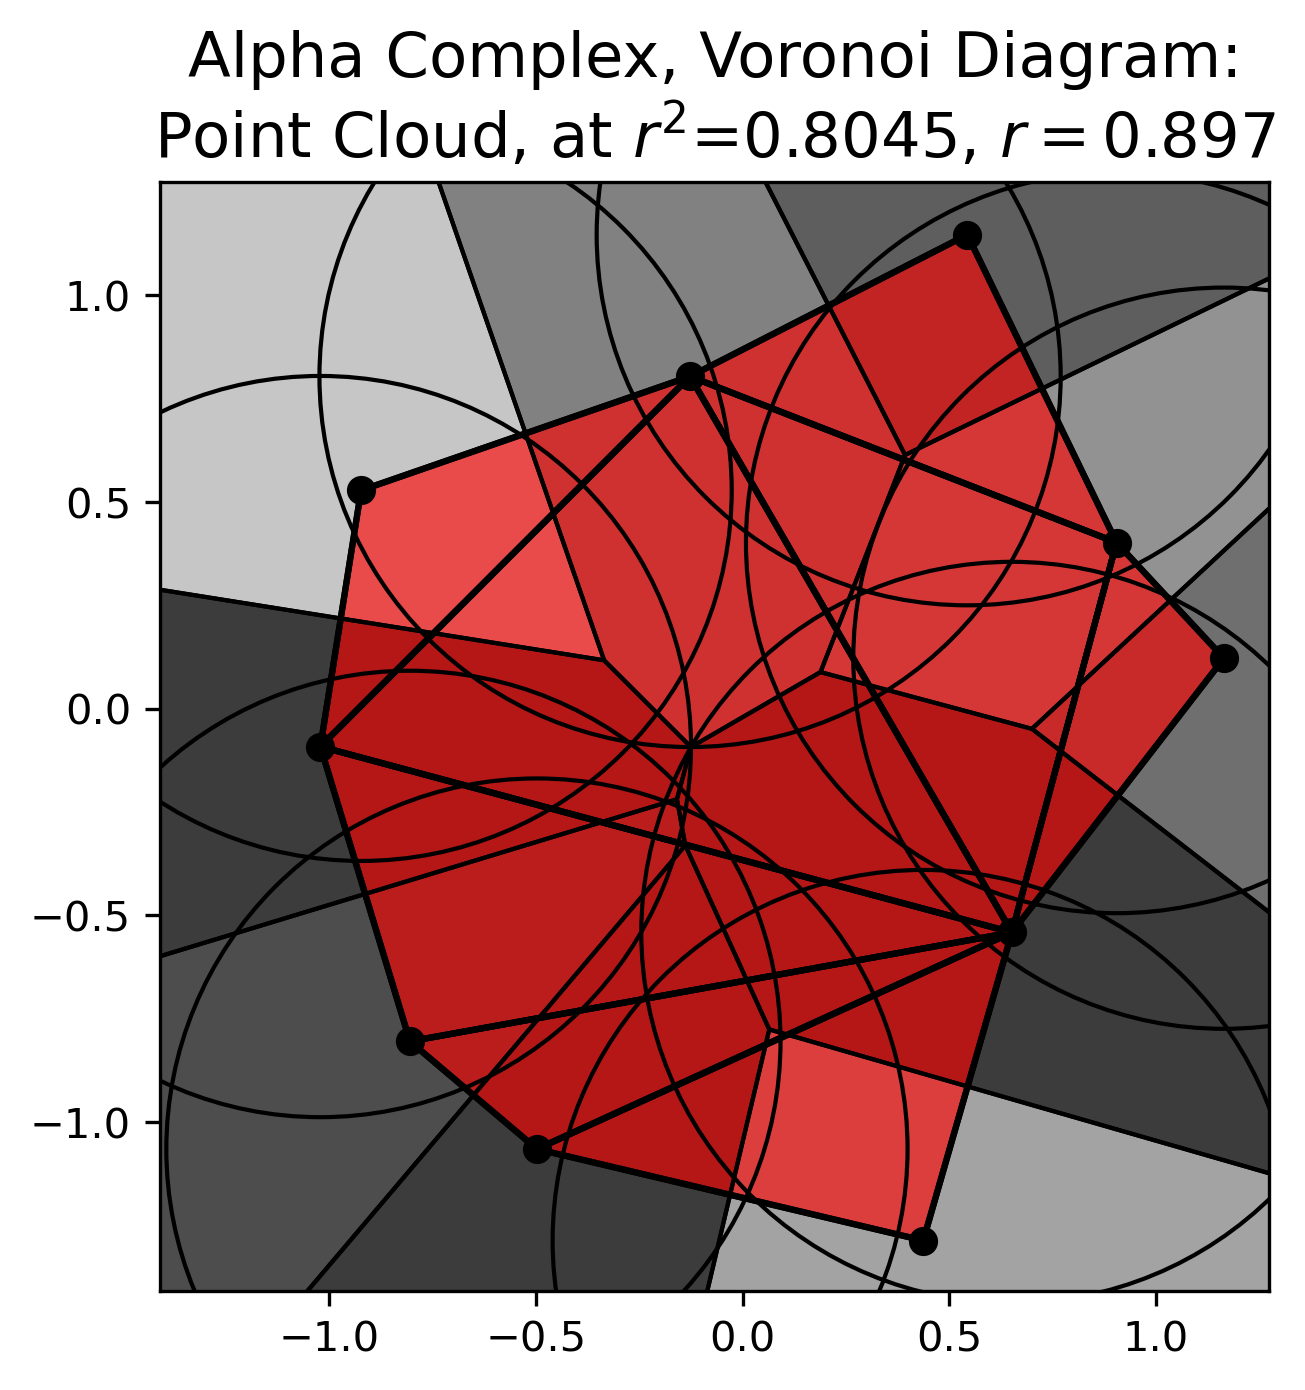
\includegraphics[width=\textwidth]{point_cloud_plot_alpha_6.png}
    \end{subfigure}
    \begin{subfigure}[b]{0.26\textwidth}
        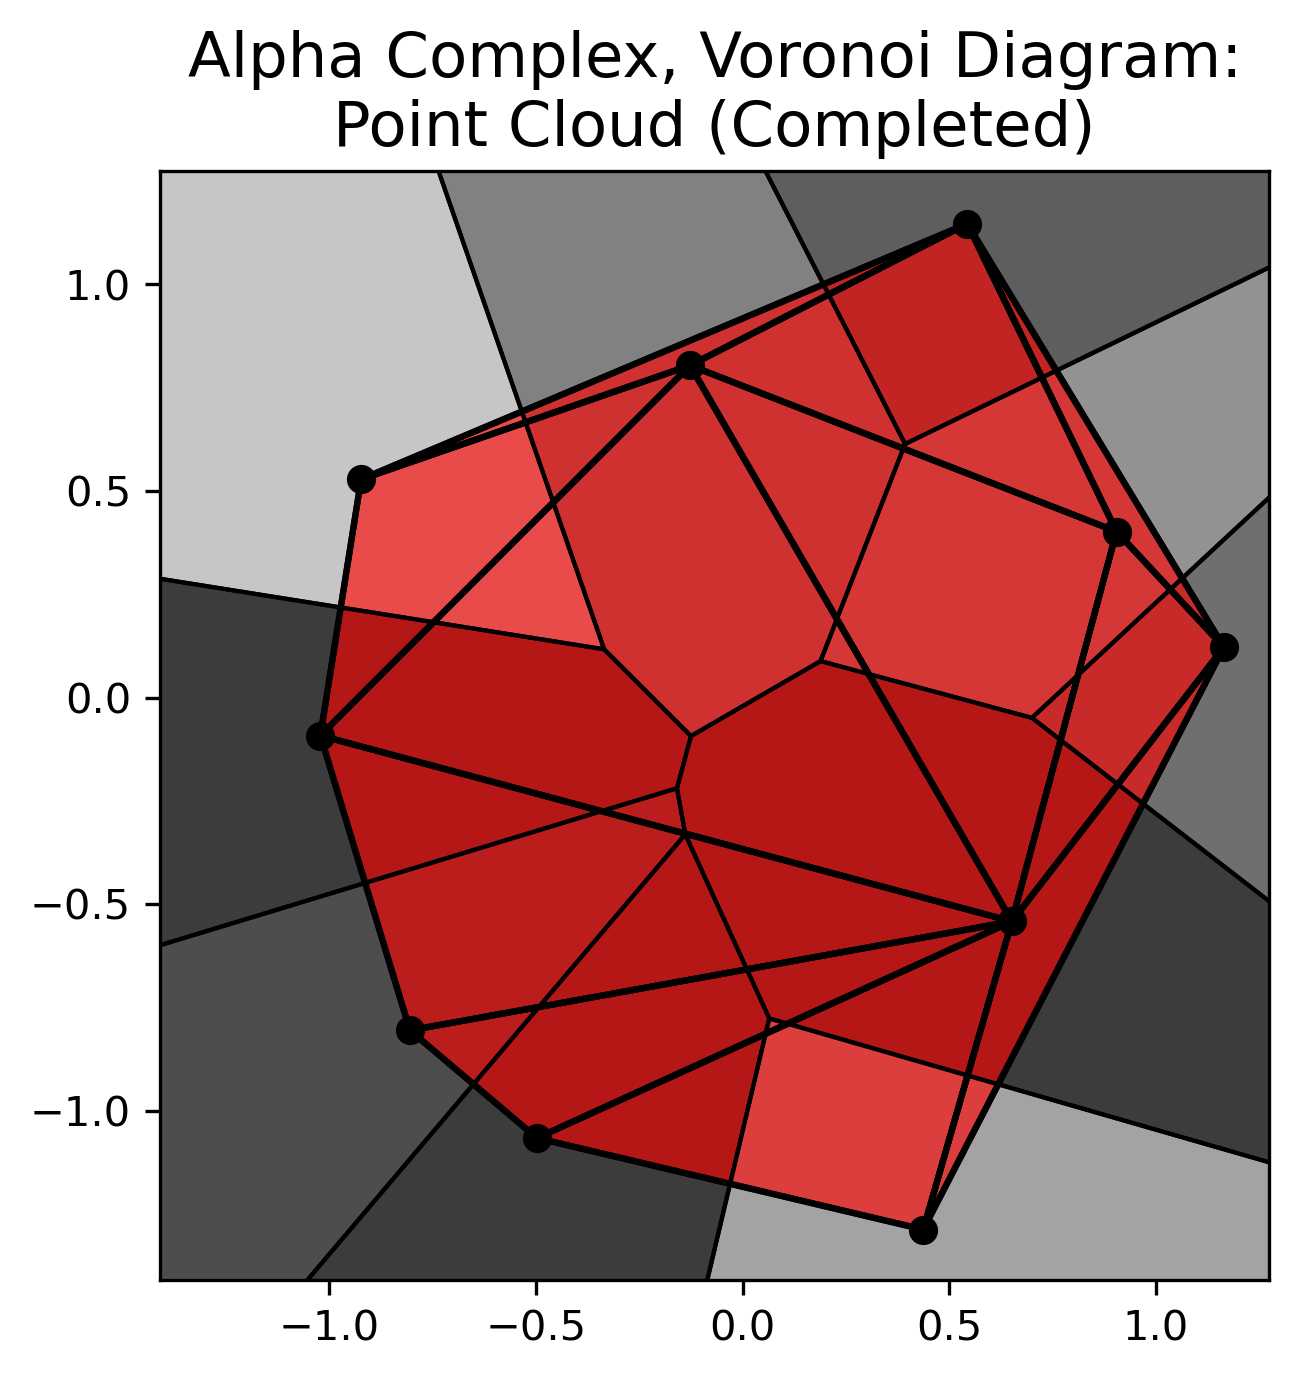
\includegraphics[width=\textwidth]{point_cloud_plot_alpha_voronoi.png}
    \end{subfigure}
    \begin{subfigure}[b]{0.26\textwidth}
        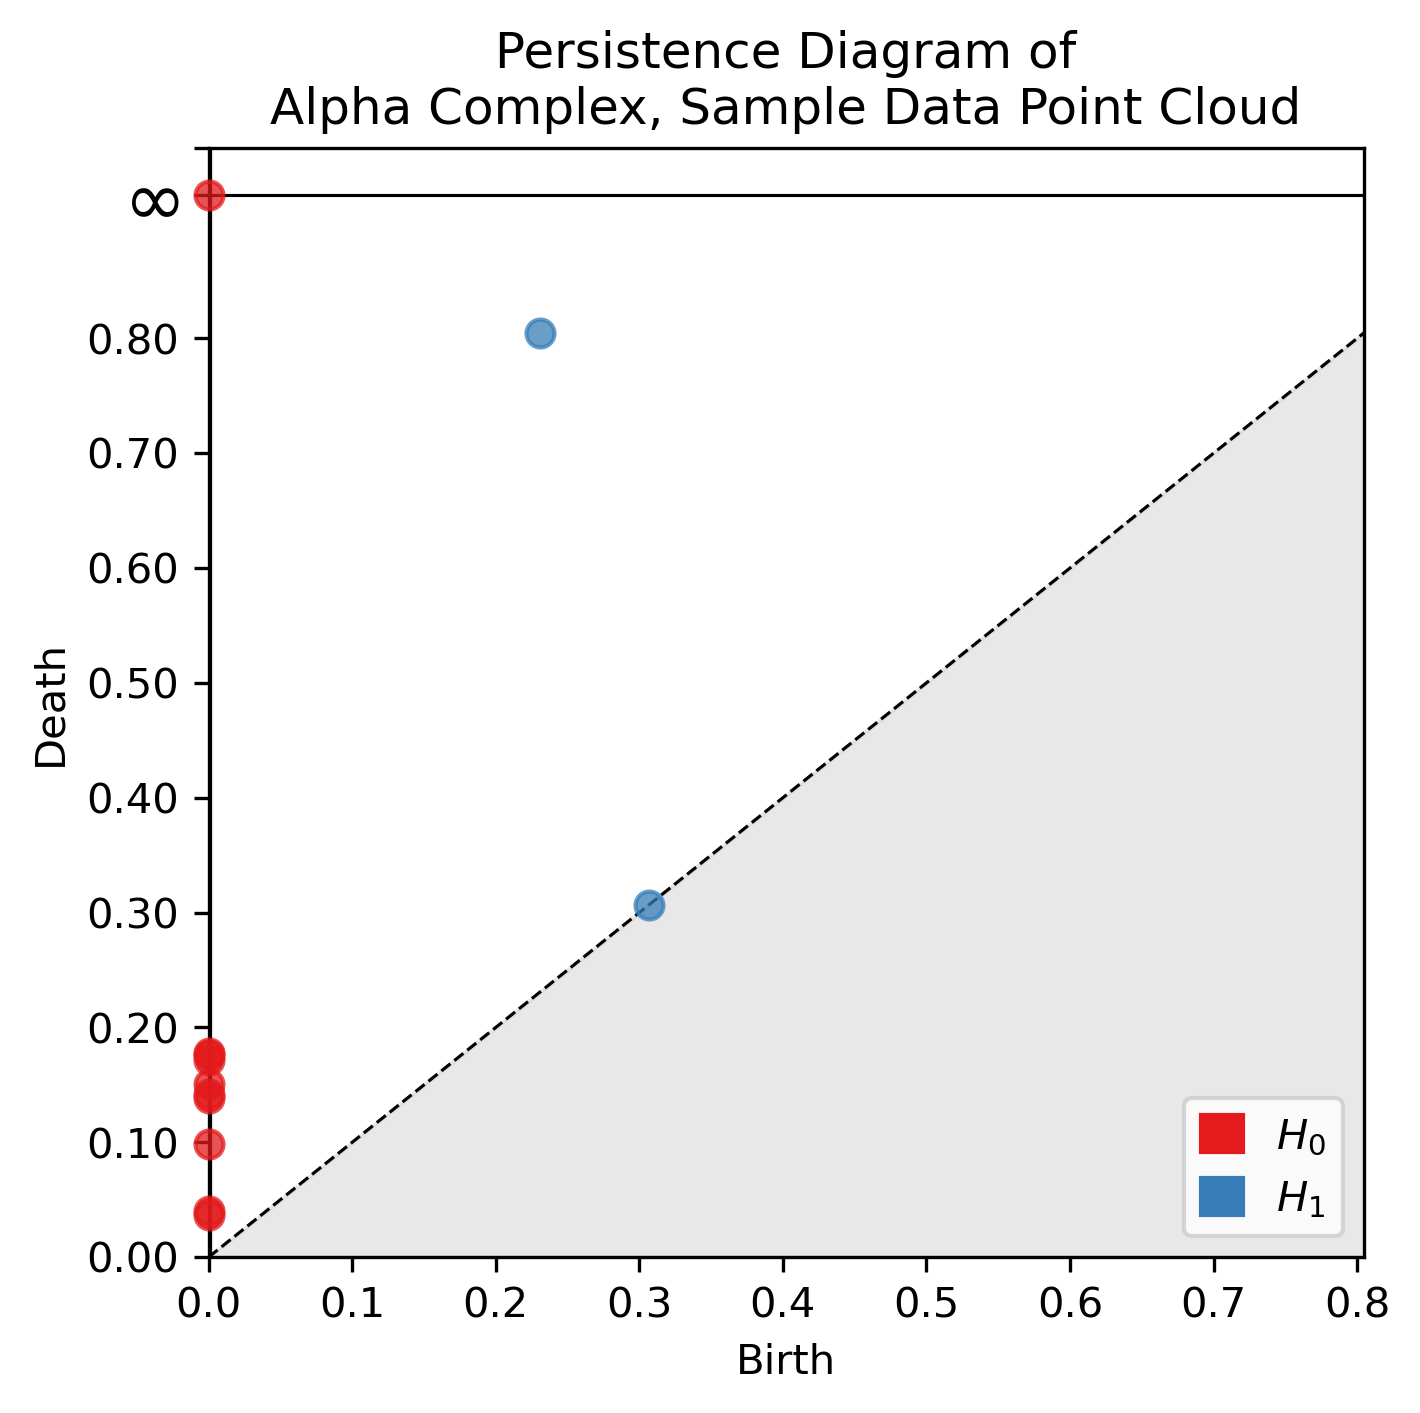
\includegraphics[width=\textwidth]{point_cloud_persdia_alpha_voronoi.png}
    \end{subfigure}

    \caption{Progression of the Alpha complex on a point cloud and the persistence diagram of the completed complex.}
    \label{fig:point_cloud_alpha_complex}
\end{figure}
\end{example}

\newpage
\begin{example}[Persistence Diagram of an Image]
\par Fig \ref{fig:image_data_persdia} uses a grayscale image of a white square with a black circle in the center to create a persistence diagram from an Alpha complex. Unlike previous examples, the dataset that creates the image is not a point cloud but is image data as a $50\times50$ array of decimal values. The white pixels in the image contain values of 1.0 and the black pixels contain no data, or values of 0.0. This causes the black circle to appear as a hole in the data.
\par This hole can be seen as a point in $H_1$ with a birth time of 0 and a radius of 10 pixels. As $r$ increases to a Euclidean distance of 10, the hole gets filled in because balls on the circumference of the black hole finally intersect. The intersection at $r=10$ is shown as a death time of ${r}^2 = 100$.
\par On a persistence diagram, in most cases, the points along or relatively close to the diagonal line which are not on the $y$-axis can be considered noise and disregarded.
\begin{figure}[H]
    \centering
    \begin{subfigure}[b]{0.45\textwidth}
        \centering
        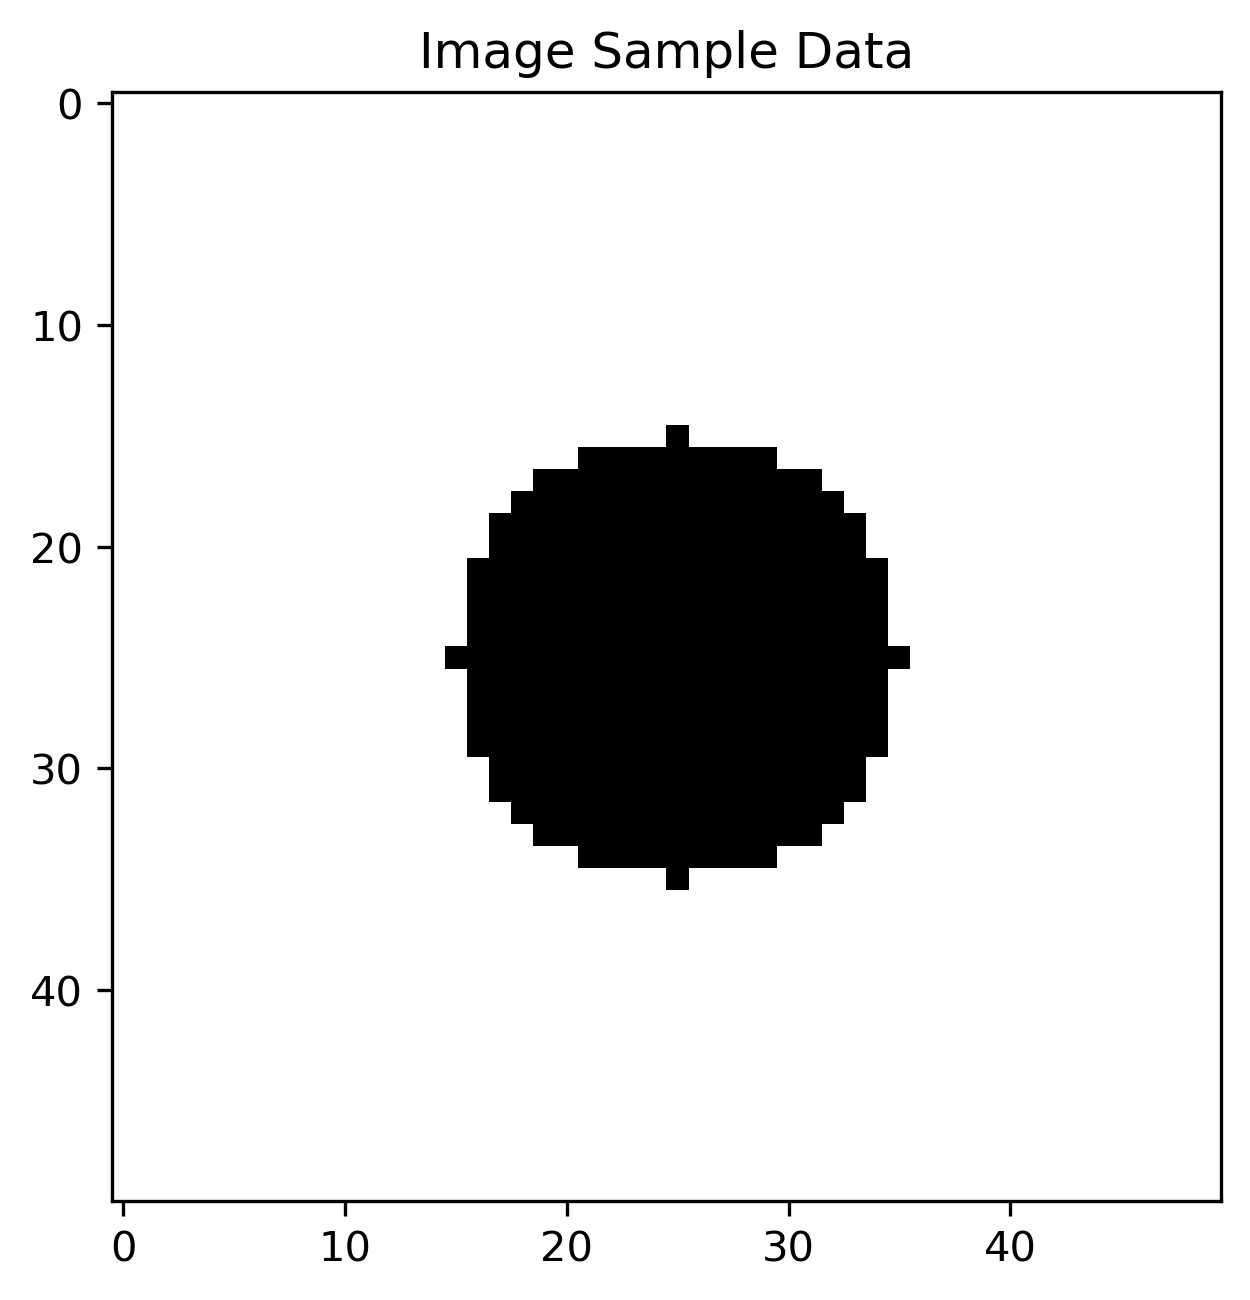
\includegraphics[width=\textwidth]{image_data_plot.png}
    \end{subfigure}
    \begin{subfigure}[b]{0.5\textwidth}
        \centering
        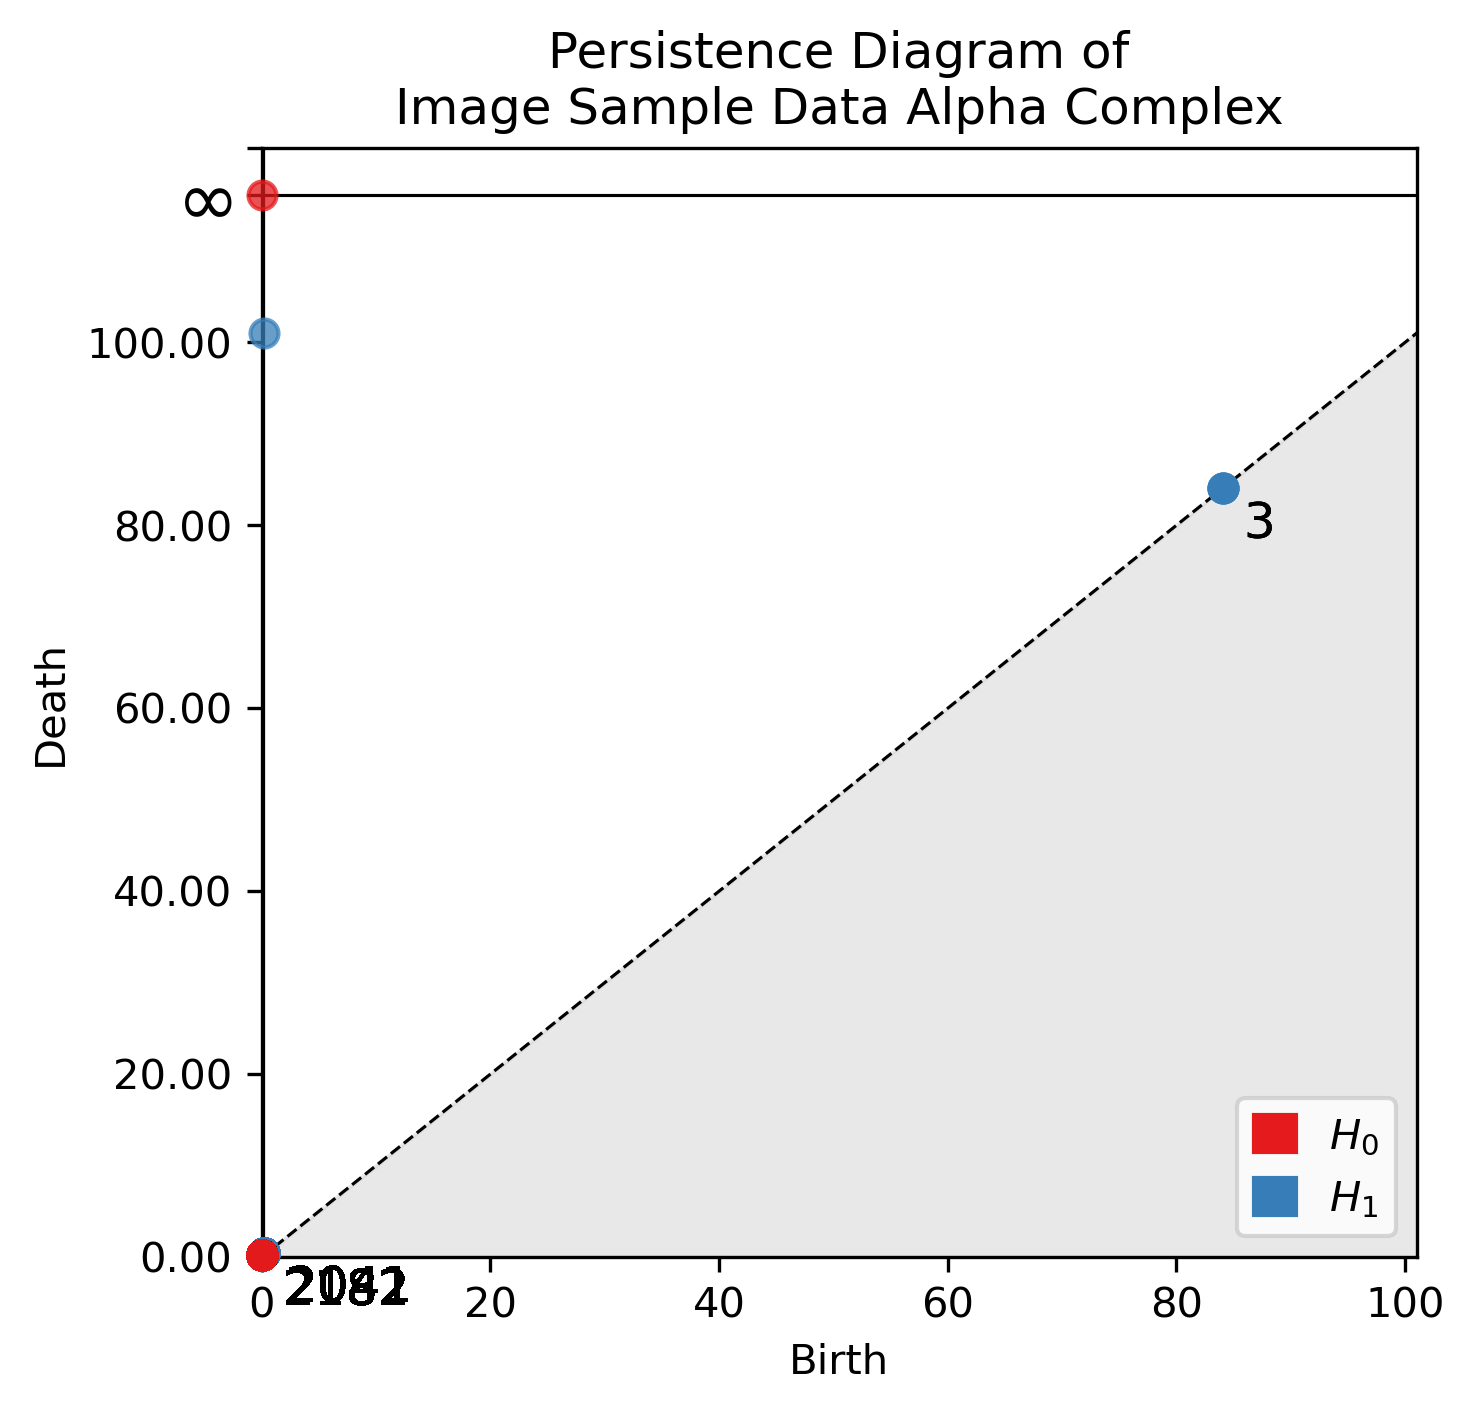
\includegraphics[width=\textwidth]{image_data_persdia.png}
    \end{subfigure}
    \caption{Plot of a white square with a hole and persistence diagram of its Alpha Complex.}
    \label{fig:image_data_persdia}
\end{figure}
\end{example}
\newpage
\section{Background on the STL Filetype}
\par An STL file is a filetype created for use with 3D data generated by computer-aided design (CAD) programs for 3D printing and other rapid-prototyping applications. STL is ancronym which can be an abbreviation for Stereolithography, Standard Triangle Language, or Standard Tesselation Language. These files are built through triangulation: every set of points creates a triangle which acts as a facet of the object. These triangles are "filled-in" 2-simplices, and will be fundamental in analyzing the topology of STL files. In terms of the contents of an ASCII STL file, a facet should not be confused with a face: a facet must be a triangle, while a face of a polyhedron can be subdivided into multiple facets to achieve triangulation. The information in an STL file can be encoded using binary or in ASCII as a \verb".ast" (ASCII STL) file. For our purposes, we will be using \verb".ast" files to extract and analyze 3D object data \cite{analysis_of_stl}.

\begin{figure}[H]
    \begin{center}
    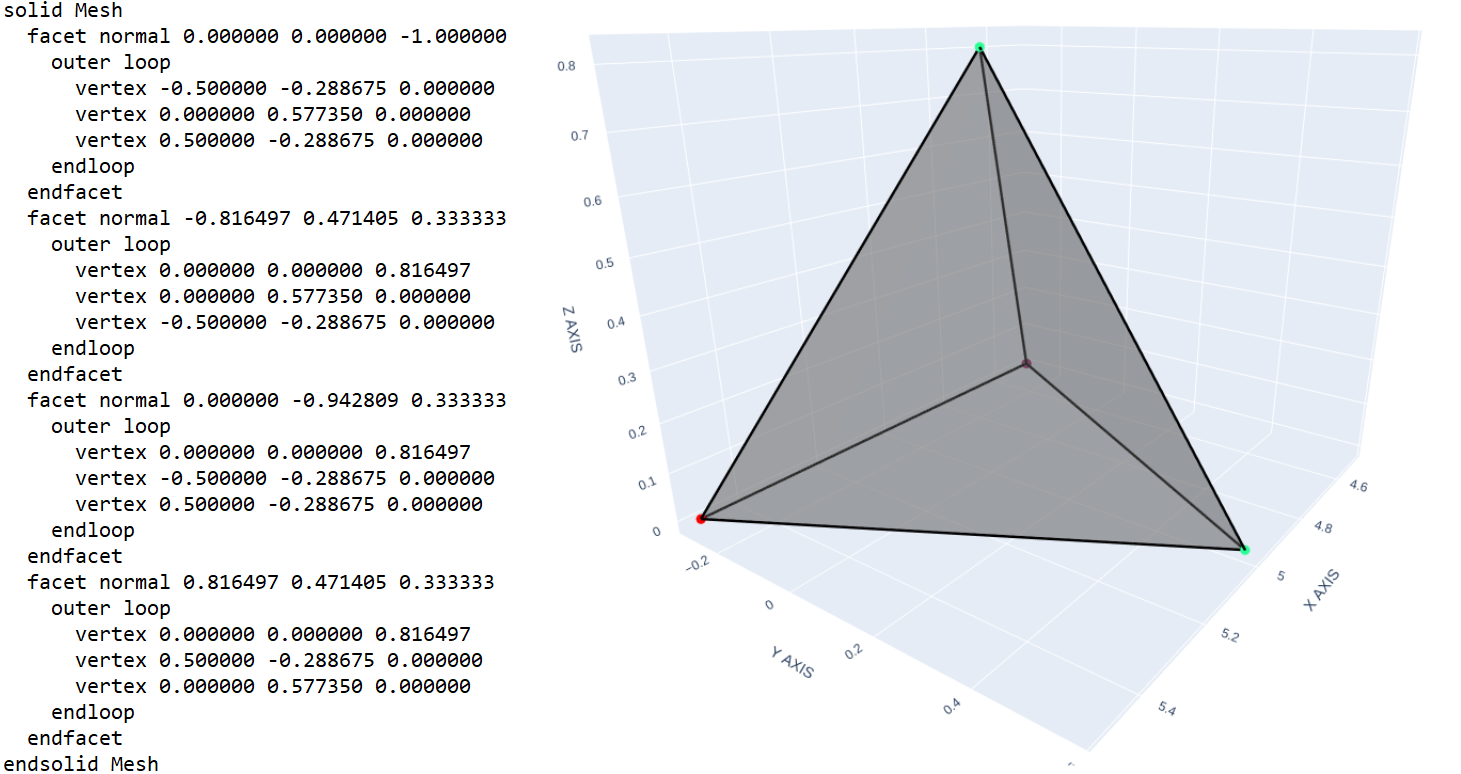
\includegraphics[height=2.9in]{tetrahedron_ast_code_and_plot.png}
    \caption{The contents and 3D plot of an ASCII STL file for a tetrahedron.}
    \label{fig:ast_tetrahedron}
    \end{center}
\end{figure}
\vspace{-7.5mm}

\par STL files contain descriptions of individual vertices, each of which are encapsulated its facet with its normal vector, as seen in the example tetrahedron, Fig \ref{fig:ast_tetrahedron}. The contents of an STL file do not specify topological information, such as connections to other vertices, which vertices make up a face, etc. Instead, STL files describe each vertex as many times as it appears in the file until the overall shape is built.

\par To analyze the topological data within STL files, we can parse the \verb".ast" files for four strings which are used to denote the beginning and end of the description of facets and vertices: 'facet normal', 'end facet', 'outer loop', and 'end loop', respectively. The data between these strings was then converted into a tuple using python.

\chapter{Methods}\label{chap:methods}
\section{Main Method}
\subsection{Creating a Mesh from an STL file}
\label{sec:mesh_from_stl}
\par To compute the persistence of the variations of the "truth" of an STL file, the data must be processed and transformed with meshing in order to be properly analyzed. Although STL files contain a mesh upon creation, this mesh is not adequate for our purposes as the triangulated mesh an STL file contains is not necessarily a subcomplex of the Delaunay triangulation. We will call a simplex a \textit{Delaunay simplex} if it is contained in the Delaunay triangulation of the vertices of the mesh. A simplicial complex is called a \textit{sub-Delaunay complex} if every simplex in it is Delaunay. The completed Alpha complex of a mesh is its Delaunay triangulation, so we require the 3D object's original mesh to be sub-Delaunay because in the next step of our method we will alter the filtered simplicial complex based on the data of the initial simplicial complex, $K_{0}$. $K_{0}$ will be compared with the Alpha complexes as $r^2$ grows to include new simplices. Without $K_0$ being sub-Delaunay, our filtration and subsequent persistence analysis may show incorrect results. 

\begin{example}[Comparison of ASCII STL mesh and Delaunay Triangulation Mesh] Fig \ref{fig:ast_circumsphere} shows the open circumsphere of a facet, emphasized by three large black points, and its circumsphere on the original triangulation for an ASCII STL file. This facet's circumsphere does contain all three vertices of the facet on its surface boundary but it also contains every vertex which makes up the hole in the center of the object within the interior of the circumsphere. This inclusion of vertices within the circumsphere means the entire object's triangulation is not Delaunay.
\par Fig \ref{fig:del_circumsphere} shows the open cirumspheres of three facets of a Delaunay triangulation of the same object. The surface boundary of each facet's circumsphere contains the three vertices of its respective facet while containing other facet vertices on its surface boundary as well. The circumsphere only containing vertices on its surface boundary but not within its interior means the object's new mesh is a Delaunay triangulation.
\begin{figure}[H]
    \centering
    \begin{subfigure}[b]{0.49\textwidth}
        \centering
        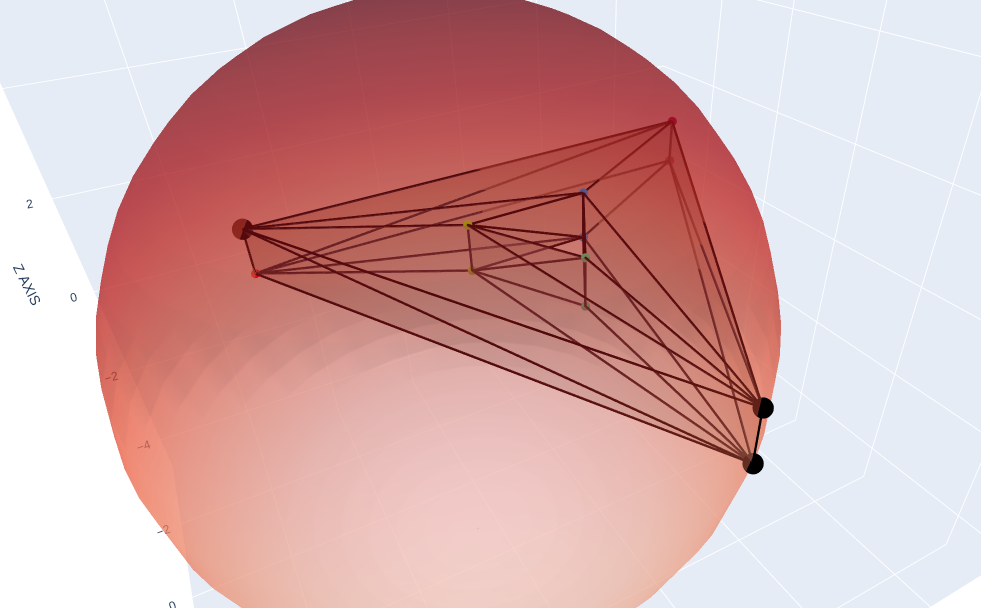
\includegraphics[width=\textwidth]{Final Run, (triangular prism - triangle hole) ast plotly screenshot circumsphere.png}
        \caption{Original mesh from ASCII STL.}
        \label{fig:ast_circumsphere}
    \end{subfigure}
    \begin{subfigure}[b]{0.49\textwidth}
        \centering
        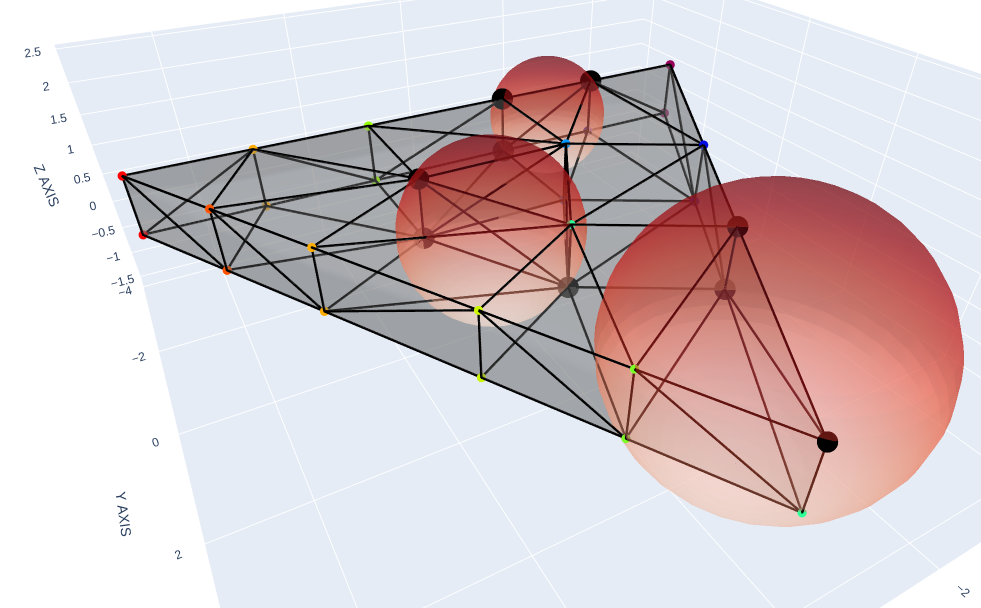
\includegraphics[width=\textwidth]{Final Run, (triangular prism - triangle hole) meshpy screenshot circumsphere.png}
        \caption{Delaunay triangulation mesh.}
        \label{fig:del_circumsphere}
    \end{subfigure}
    \caption{The original input mesh of the data from an ASCII STL file and its Delaunay triangulation mesh.}
    \label{fig:delaunay_circumsphere}
\end{figure}
\end{example}

\subsection{Creating and modifying an Alpha Complex}
\label{sec:modify_alpha_complex}
\par Now we are ready to generate an Alpha complex. The sub-Delaunay complex mesh $K_{0}$, created by the Delaunay triangulation, contains every edge and triangle present in the original 3D object mesh while retaining its boundaries, so the topology is not altered as it will be with the Alpha complex. The sub-Delaunay $K_{0}$ is a subset of the completed Alpha complex, therefore every simplex present in the $K_{0}$ complex is present as a simplex in the Alpha complex of the vertices for some scale parameter $r$.
\par The Alpha complex grows to include simplices which were not originally in the $K_{0}$ sub-Delaunay complex. These Alpha complex simplices are checked against the $K_{0}$ simplices to determine which simplices were present originally. All simplices that were present originally will be given a new filtration value of 0 to denote they appear in the $K_{0}$ complex. Replacing the filtration values in this way is done to ensure the original simplices from $K_{0}$ have a corresponding birth time of $b=0$, while all new simplices created by the Alpha complex will retain their assigned $r^{2}$ filtration.

\subsection{Computing a Persistence Diagram}
\label{sec:compute_persdia}
\par Now that we have created and reassigned the appropriate filtration values that make up our filtered simplicial complex, we compute a persistence diagram using Def \ref{def:persdia}. We then create persistence diagrams of each variation of the 3D object to see the progression of its homology over the changes to a feature or features of a part. The death axes on the sequence of persistence diagrams are constrained to the maximum death time within the sequence to keep the plots consistent and monitor its change over the variations.
\newpage
\begin{example}[Example of Methods with a Single 3D Object]
\par Fig \ref{fig:methods_example} shows the progression of transformations to the STL file data. Initially, the object is loaded in and parsed to create the 3D plot of its original mesh in Fig \ref{fig:initial_stl}. Then, the data is meshed to create a Delaunay Triangulation (additional points are added to the mesh which will be expanded on in Sec \ref{sec:implement_meshpy}) in Fig \ref{fig:meshpy_of_stl}. Finally, we compare the simplices in \ref{fig:meshpy_of_stl} to the simplices in the alpha complex of the meshed 3D object and plot its persistence in \ref{fig:persdia_of_stl} to show 1 connected component in $H_{0}$ and 1 hole in $H_{1}$.
\begin{figure}[H]
    \centering
    \begin{subfigure}[b]{0.3\textwidth}
        \centering
        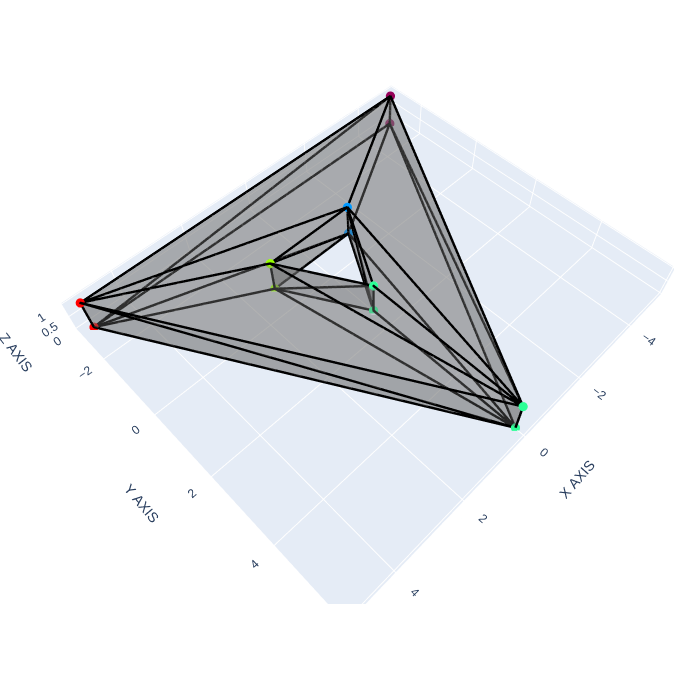
\includegraphics[width=\textwidth]{Final Run, (triangular prism - triangle hole) ast plotly screenshot.png}
        \caption{}
        \label{fig:initial_stl}
    \end{subfigure}
    \hfill
    \begin{subfigure}[b]{0.3\textwidth}
        \centering
        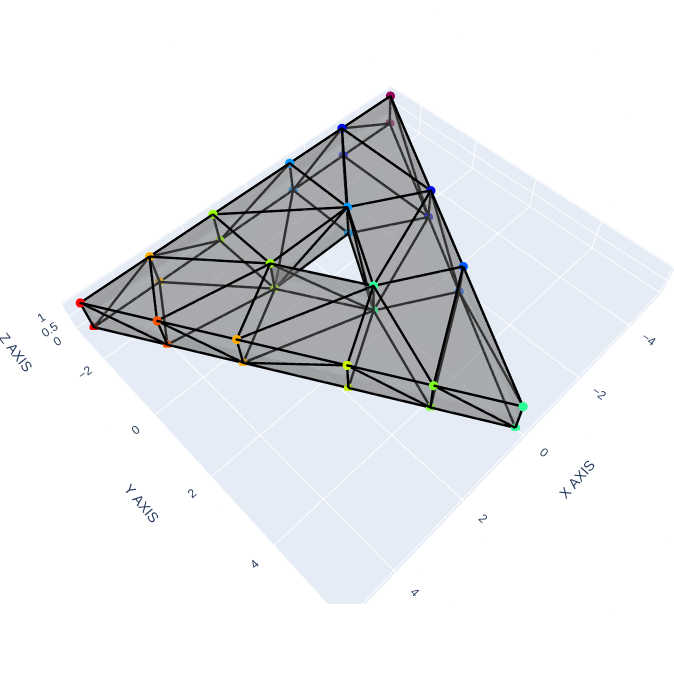
\includegraphics[width=\textwidth]{Final Run, (triangular prism - triangle hole) meshpy screenshot.png}
        \caption{}
        \label{fig:meshpy_of_stl}
    \end{subfigure}
    \hfill
    \begin{subfigure}[b]{0.3\textwidth}
        \centering
        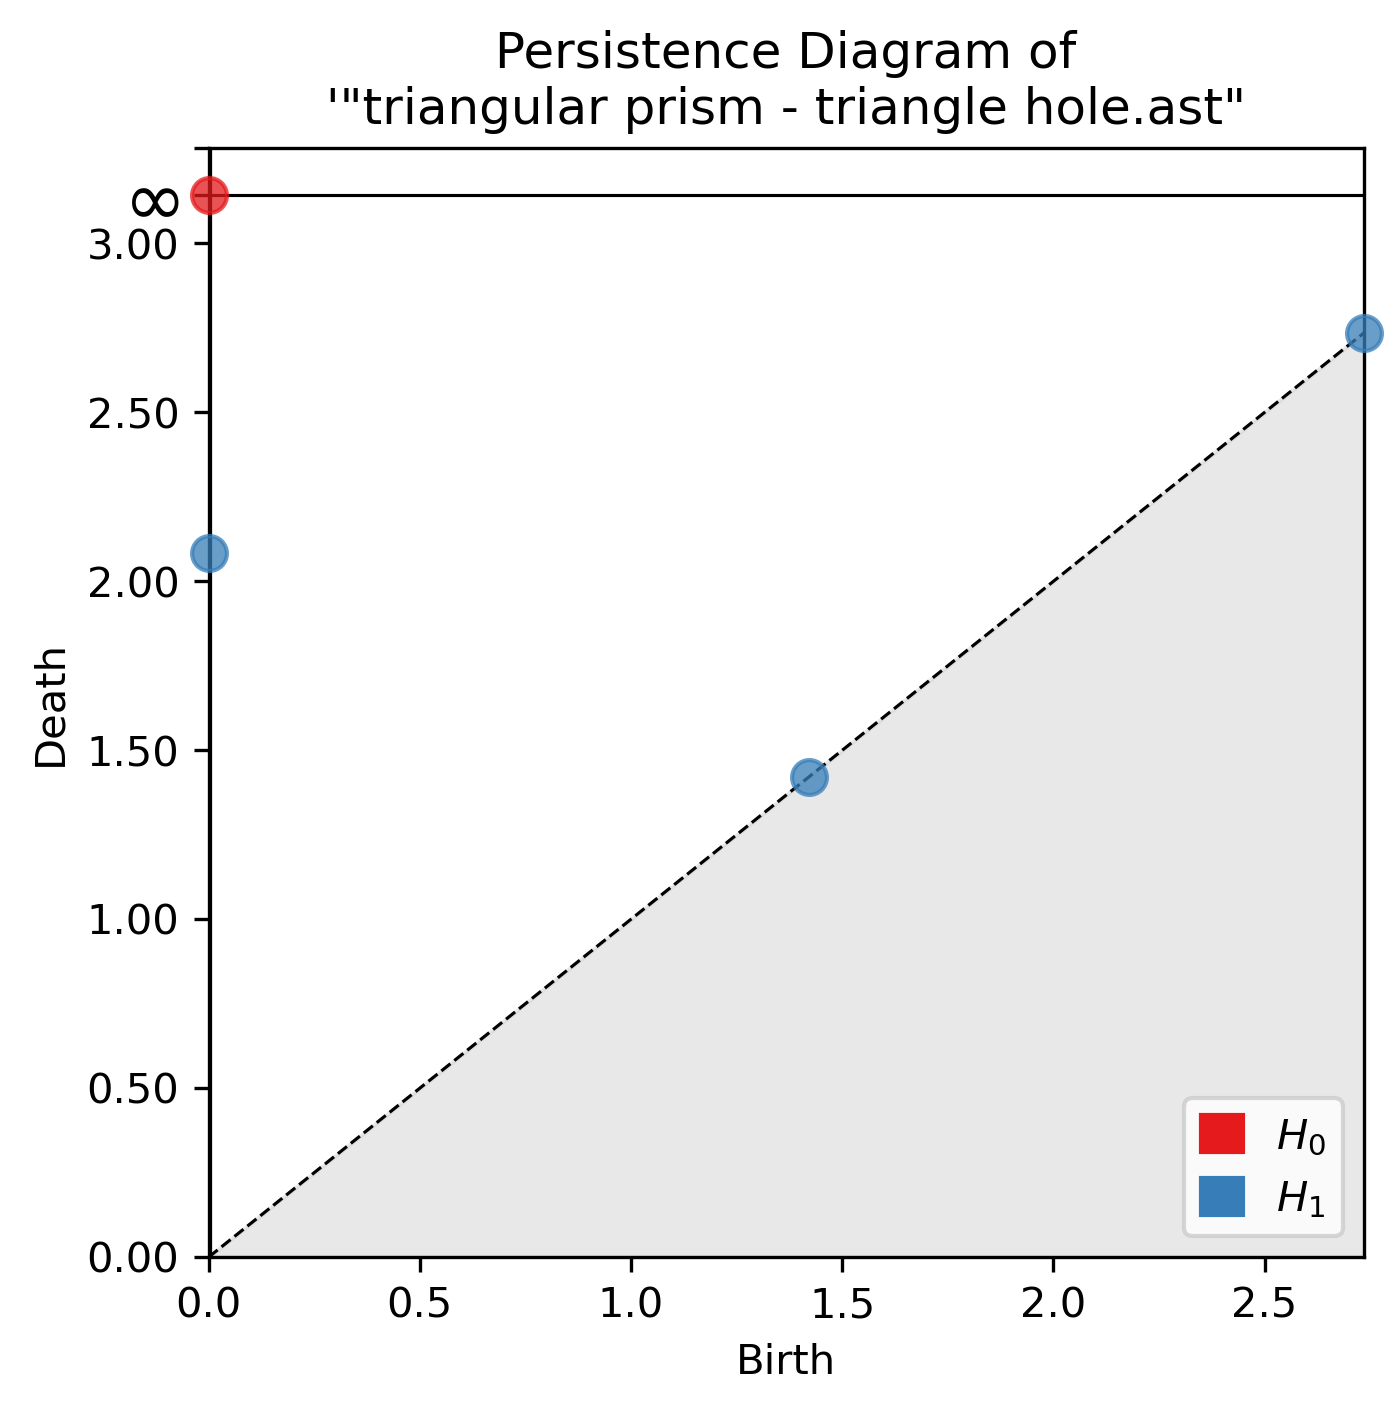
\includegraphics[width=\textwidth]{Final Run, (triangular prism - triangle hole) persdia.png}
        \caption{}
        \label{fig:persdia_of_stl}
    \end{subfigure}
    \caption{A triangular prism with a triangular hole, its Delaunay triangulated mesh, and the persistence diagram of the Delaunay triangulated mesh}
    \label{fig:methods_example}
\end{figure}
\end{example}

\section{Implementation}

\par The methods of this paper are implemented in Python using many libraries, most notably \verb"MeshPy" for mesh creation, \verb"Gudhi" for TDA, \verb"Plotly" to visualize 3D plots, and \verb"Matplotlib" to visualize persistence diagrams.

\subsection{Creating STL Files with FreeCAD}
\par STL files from online sources such as Thingiverse can be processed through the program, but these files are often too complex and therefore very computationally expensive. For this reason, we create our own dataset to test our methods using FreeCAD to keep complexity to a minimum while covering basic test cases that demonstrate potential tolerancing errors. The parts are all exported to an ASCII STL (\verb".ast") which encodes the data as text to allow for the data to be easily read in by Python.

\subsection{Parsing the STL File Data}
\par We will discuss two methods to load in the data an ASCII STL file. We can parse data directly from the \verb".ast" file and load it into lists and tuples, or we can use the \verb"load_stl()" attribute of the \verb"MeshPy" \verb"MeshInfo" object.

\par For "simplicity", we will use the \verb"load_stl()" attribute. To use this method with a \verb".ast" file, we will pass in the full file path of the \verb".ast" file, but first we must use Python to create a temporary copy with the extension renamed to \verb".stl" even though the content of the file will stil be ASCII text. Without creating a temporary copy that renames the \verb".ast" to \verb".stl", \verb"load_stl()" will not work. This temporary \verb".stl" file is then passed in to \verb"load_stl()" to create our \verb"MeshInfo" object which will be used to build the new Delaunay triangulation mesh.

\par Although we use \verb"MeshPy" to load in the data, the following paragraph is an example of how ASCII STL file data could be loaded in if we wanted to do it manually. Loading in the code manually can be advantageous if we want to directly alter the ASCII STL data of the chosen "truth" \verb".ast" file to create variations of part features by manipulating the facets and vertices and saving these manipulations as new \verb".ast" files to be analyzed sequentially.

\par As shown in Fig \ref{fig:ast_tetrahedron}, an ASCII STL file is delimited by the formatting of its facets and vertices. We use the strings 'facet normal', 'end facet', 'outer loop', 'end loop', and newline character delimiters to identify the faces and vertices of the 3D object. For each facet, the ASCII data gives us the normal vector of the facet and the coordinates of each of the three points that makes up the facet. At this point, we can use the parsed data to add or manipulate points, edges, or facets if we choose to do so. We can then use the parsed or manipulated data to create a list of points where each unique point is numbered numerically. All point names would be 1-indexed, or begin naming at 1, to match the indexing of \verb"Gudhi". The list of unique edges can be extracted from the list of facets and matched with their vertex names to create a list of edges described by two vertex names instead of coordinates. The same can be done to describe each facet by the three vertex names that create it. This relational point name data can then be passed in to \verb"Gudhi" if the triangulation is Delaunay.

\cprotect\subsection{Creating a Delaunay Triangulation with \verb+MeshPy+}
\label{sec:implement_meshpy}
\par \verb"MeshPy" is a library that creates meshes by adapting the TetGen mesh generation program to python. As per the TetGen documentation \cite{tetgen}, Tetgen creates Delaunay tetrahedralizations (triangulations for our purposes) by default. Additional switches can be added to the code to enhance or alter the mesh. While there are dozens of possible switches to use, for simplicity, we will only be using \verb"-p" and \verb"-q".
\newpage
\cprotect\subsubsection{Switch \verb+-p+: Tetrahedralize a Piecewise Linear Complex}
\par The switch \verb"-p" Tetrahedralizes a piecewise linear complex (PLC). According to the documentation, a PLC is defined as the following:

\begin{definition}[Piecewise Linear Complexes]
\par A 3D \textit{piecewise linear complex} $\mathcal{X}$ is a set of cells that satisfies the following properties:
\begin{enumerate}
\item The boundary of each cell in $\mathcal{X}$ is a union of cells in $\mathcal{X}$
\item If two distinct cells $f, g \in \mathcal{X}$ intersect, their intersection is a union of cells in $\mathcal{X}$.
\end{enumerate}
\par The boundary of a 3D PLC is the set of cells whose dimensions are less than or equal to 2:
\begin{enumerate}
\item A 0-dimensional cell is a vertex
\item A 1-dimensional cell is a segment, or an edge
\item A 2-dimensional cell is a facet
\end{enumerate}
\end{definition}

The \verb"-p" is how Fig \ref{fig:delaunay_circumsphere} retains its original shape's boundary but consists of new points and edges to allow for the mesh to be Delaunay. However, the specific Delaunay triangulation used with this switch is a Constrained Delaunay Tetrahedralization (CDT - again, triangulation for our purposes). A CDT differs slightly from a Delaunay triangulation in that open circumspheres of facets on the outer surface of a mesh are allowed to contain other facet's vertices on its surface boundary, as seen in Fig \ref{fig:del_circumsphere}.

\cprotect\subsubsection{Switch \verb+-q+: Refine Mesh}
\par The \verb"-q" switch can be used in combination with \verb"-q" to improve the quality of the mesh by inserting additional points into the mesh. This is done with two constraints. The first constraint is a \textit{maximum radius-edge ratio bound}. This ratio is found by dividing the radius of the circumsphere of a tetrahedron (facet, in our case) by the length of the shortest edge of that facet. This constraint limits the maximum ratio up to a default value of 2.0. A smaller ratio means more triangulations will be made. The second constraint is a \textit{minimum dihedral angle bound}. A dihedral angle is the angle between two planes. This constraint has a default value of 0 degrees. Choosing a larger minimum dihedral angle bound will cause the facets to be larger than they would be otherwise.

\cprotect\subsection{Creating and modifying an Alpha Complex with \verb+Gudhi+}
\par \verb"Gudhi" is a python library which contains functions to analyze the topology of a dataset. We will be using it to do this through generating an Alpha complex and modifying it as outlined in Sec \ref{sec:modify_alpha_complex}. By comparing the simplices of the Delaunay triangulation mesh generated by \verb"MeshPy" and the simplices of the alpha complex generated by \verb"Gudhi", we change the filtration values so that every original simplex from the Delaunay triangulation has a filtration value of 0 and appears in $K_{0}$, while the remaining simplices generated from the Alpha complex will retain their assigned filtration.

\subsection{Persistence Diagram Construction}
\par Using the \verb"Matplotlib" python library in tandem with the persistence points generated by \verb"Gudhi", we create a persistence diagram, like the persistence diagram of the tetrahedron from Fig \ref{fig:ast_tetrahedron}. We will use a sequence of diagrams to show the progression of change in the topology of variations of 3D object features.
\begin{figure}[H]
    \begin{center}
	    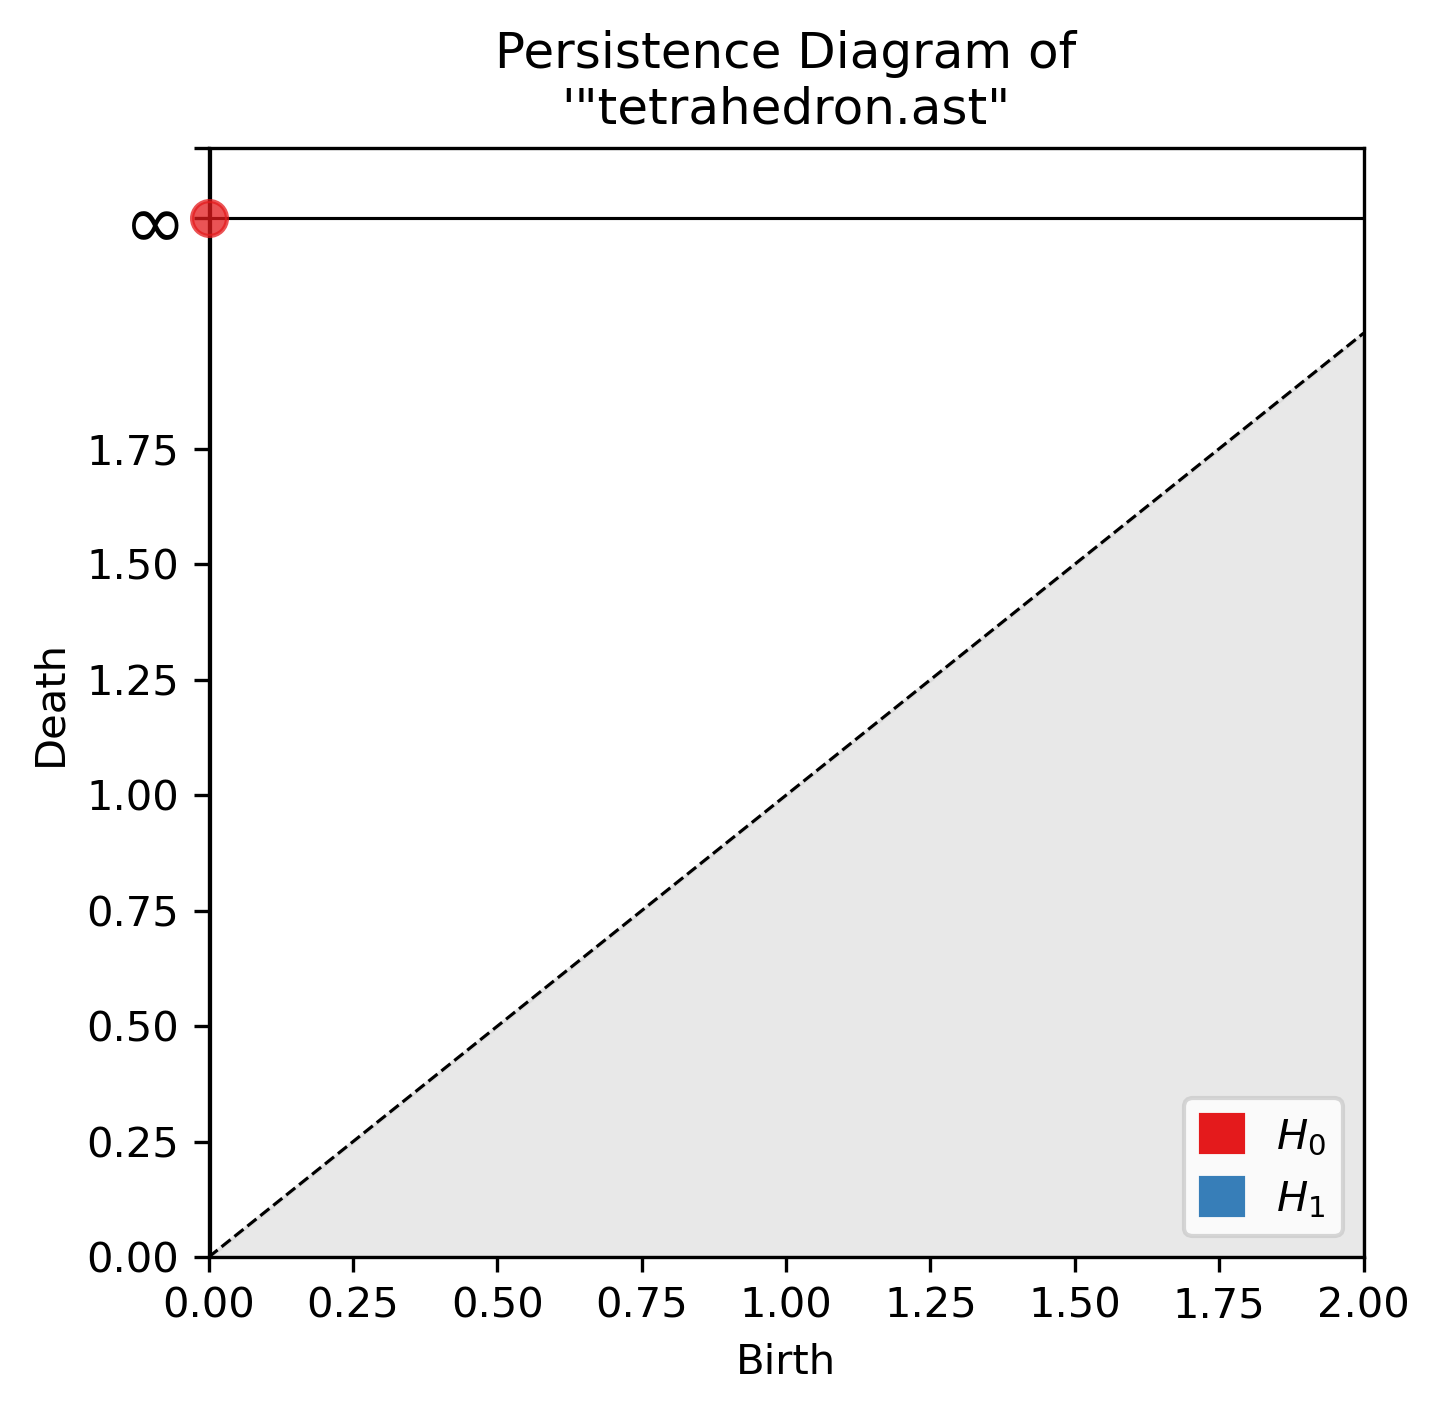
\includegraphics[width=0.45\textwidth]{tetrahedron persdia.png}
    	\caption{Persistence diagram of a tetrahedron.}
    \end{center}
\end{figure}

\chapter{Results}
\par The datasets used for these experiments was created with the CAD software FreeCAD, then exported to an ASCII STL as an input to \verb"MeshPy". The images of the 3D objects are displayed with the Python library \verb"Plotly". For each experiement, a feature of a file was chosen to be manipulated by changin a measurement over a series of alternate version files. This was done to show how our method lets us observe the change in homology as these measurements change across the file variations. We will dicuss the results in Chapter \ref{chap:discussion}.

\section{Two Cubes with Three Pockets Moving Closer}
\label{sec:two_cubes}
A CAD pocket operation subtracts an area from a face by some depth. This can also create a hole which goes through an object's face. This operation was done to a cube on the top, front, and right faces to create three intersecting pockets through each face of the cube, as shown in Fig \ref{fig:three_pocket_example}.
\begin{figure}[H]
\begin{center}
	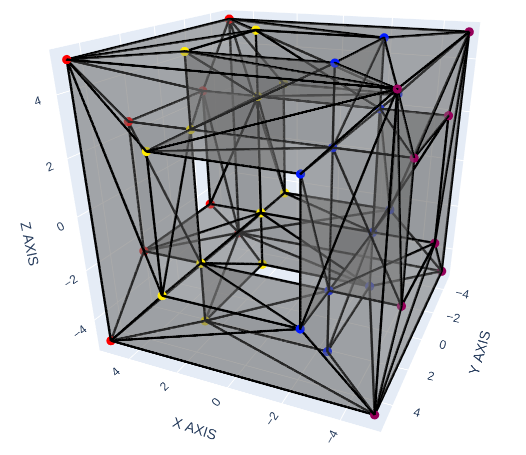
\includegraphics[width=0.45\textwidth]{one cube three pockets each.png}
    \caption{Cube with three pockets.}
\label{fig:three_pocket_example}
\end{center}
\end{figure}
\newpage
\begin{figure}[H]
    \begin{center}
    \begin{tabular}{|c|c|}
    \toprule
    \tstack{\includegraphics[height=0.875in]{Final Run, (two cubes, three pockets each, 50 mm apart) MeshPy plotly screenshots.png}\\ {\fontsize{10}{12}\selectfont 50 mm apart}}  &
    \tstack{\includegraphics[height=0.875in]{Final Run, (two cubes, three pockets each, 40 mm apart) MeshPy plotly screenshots.png}\\ {\fontsize{10}{12}\selectfont 40 mm apart}}  \\
    \midrule
	\tstack{\includegraphics[height=0.875in]{Final Run, (two cubes, three pockets each, 30 mm apart) MeshPy plotly screenshots.png}\\ {\fontsize{10}{12}\selectfont 30 mm apart}}   &
	\tstack{\includegraphics[height=0.875in]{Final Run, (two cubes, three pockets each, 20 mm apart) MeshPy plotly screenshots.png}\\ {\fontsize{10}{12}\selectfont 20 mm apart}}  \\
	\midrule
    \tstack{\includegraphics[height=0.875in]{Final Run, (two cubes, three pockets each, 10 mm apart) MeshPy plotly screenshots.png}\\ {\fontsize{10}{12}\selectfont 10 mm apart}}  &
    \tstack{\includegraphics[height=0.875in]{Final Run, (two cubes, three pockets each, 00 mm apart) MeshPy plotly screenshots.png}\\ {\fontsize{10}{12}\selectfont 00 mm apart}}  \\
    \bottomrule
    \end{tabular}
    \end{center}
    \caption{MeshPy plots displayed with Plotly of two cubes with three CAD pocket operations that move closer together until combining.}
    \label{fig:cube_two_cubes_MeshPy_table}
\end{figure}

\begin{figure}[H]
\begin{center}
    \begin{tabular}{cc}
         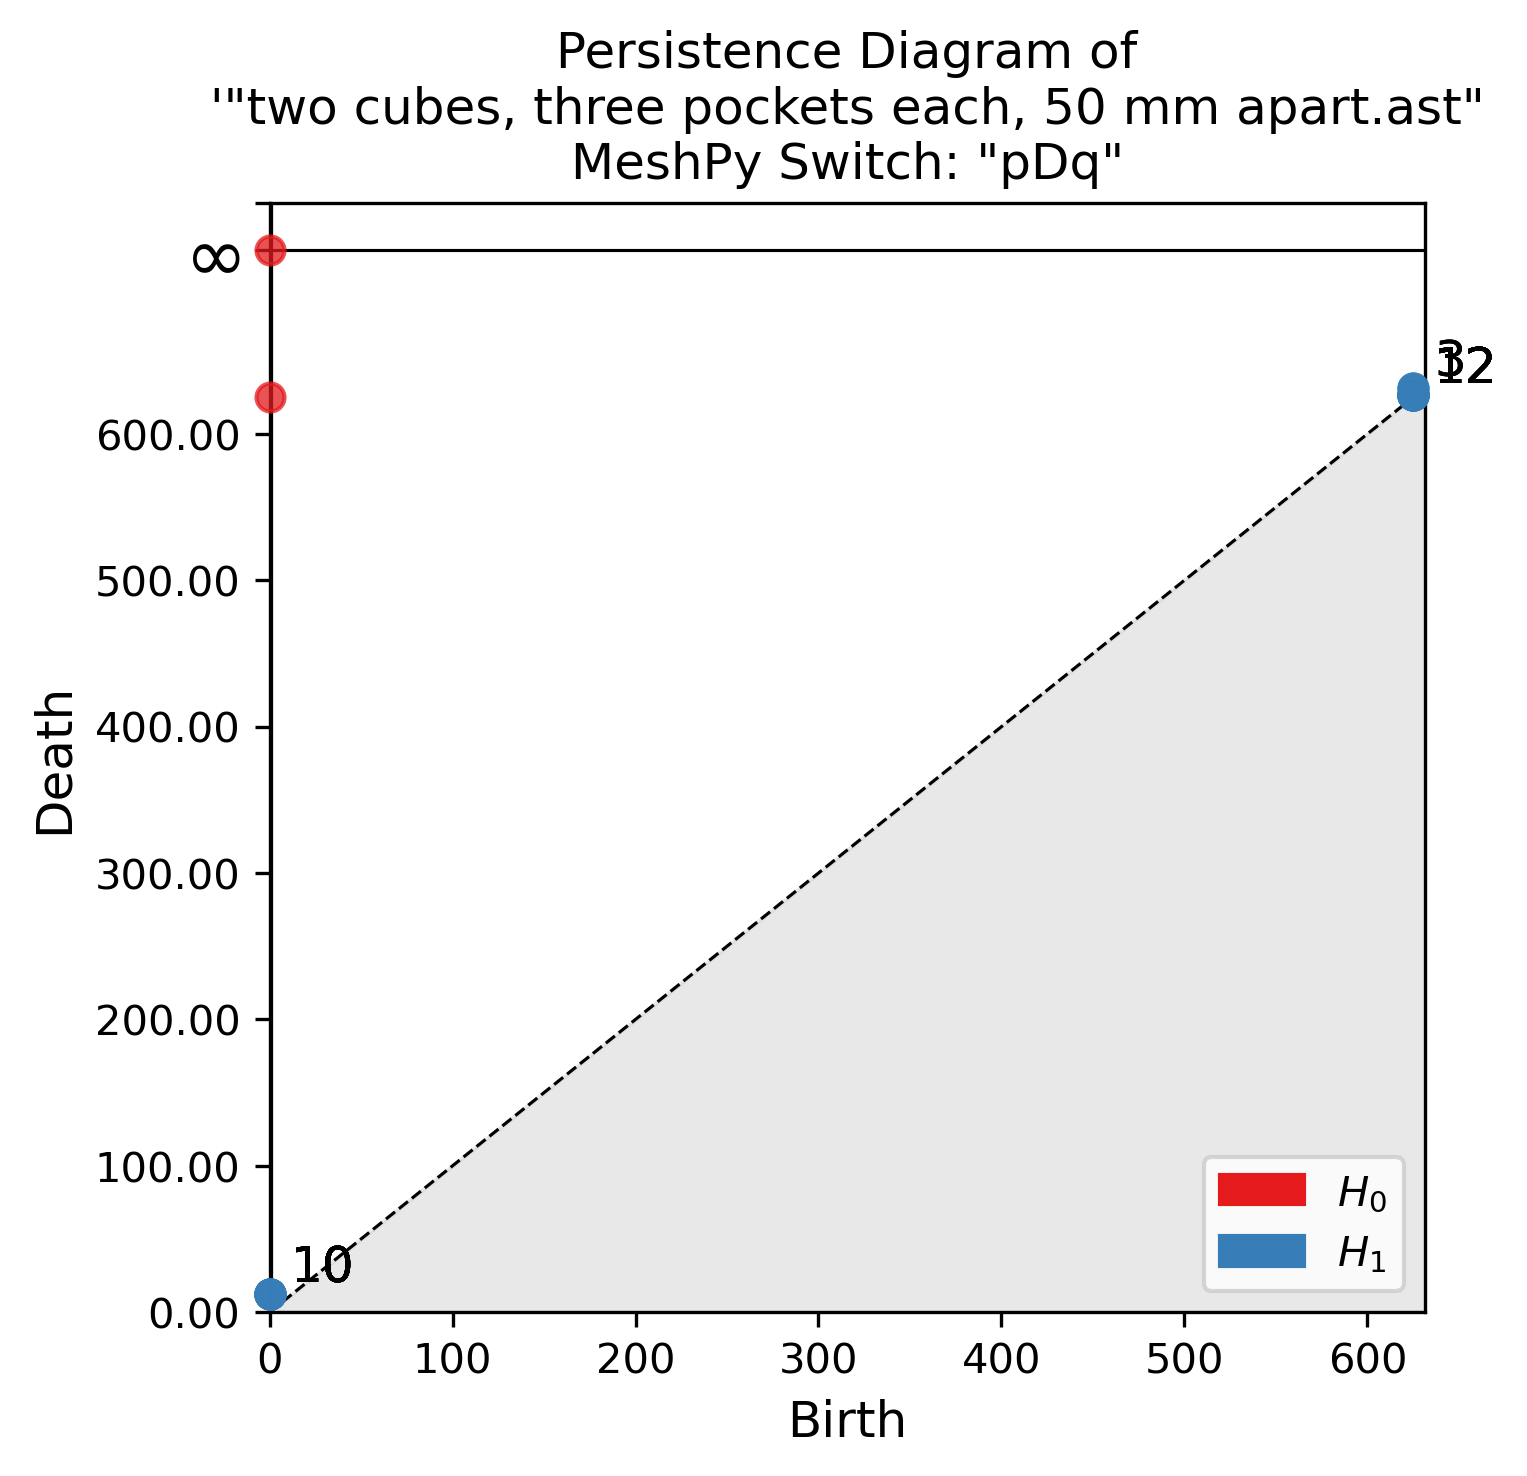
\includegraphics[width=2.5in]{Final Run, (two cubes, three pockets each, 50 mm apart) persdia.png} &
         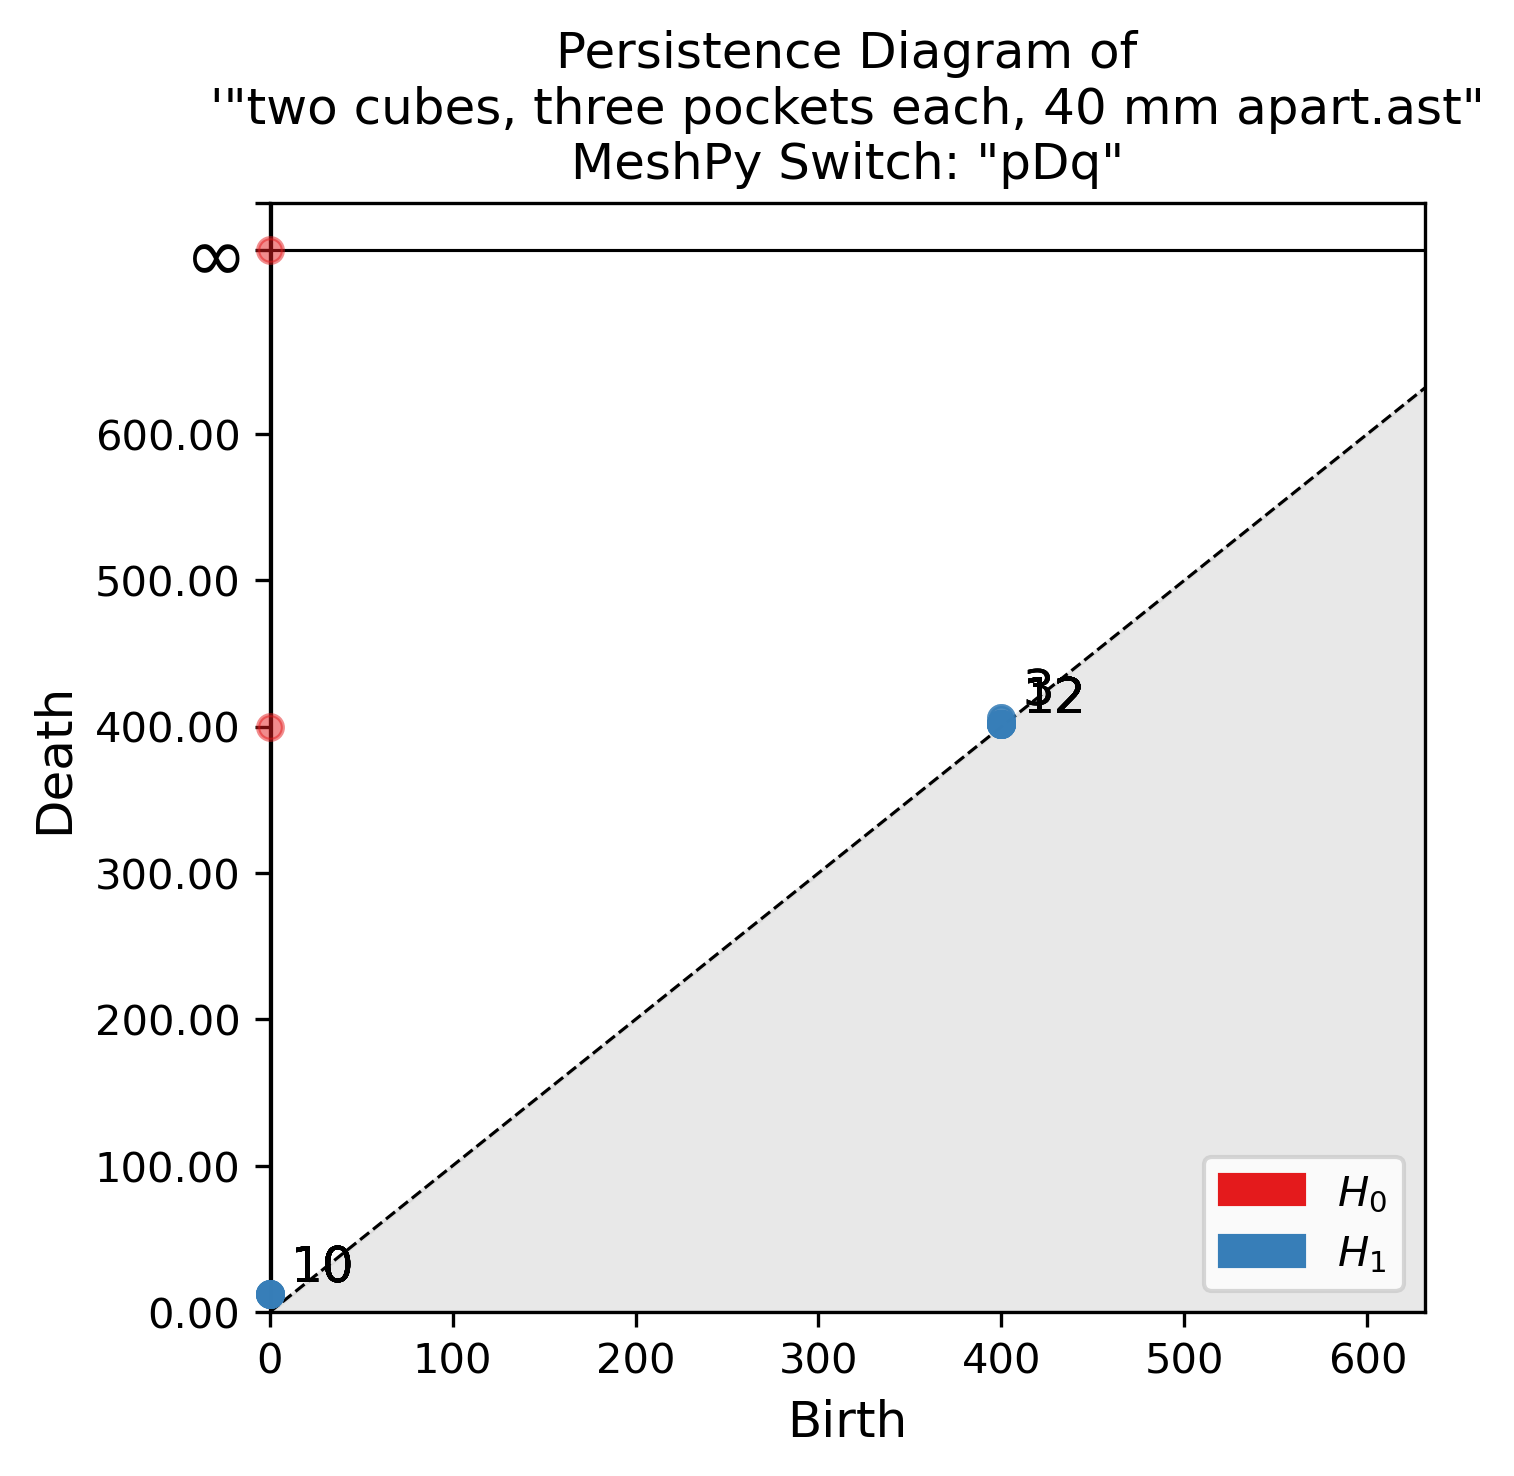
\includegraphics[width=2.5in]{Final Run, (two cubes, three pockets each, 40 mm apart) persdia.png} \\ 
         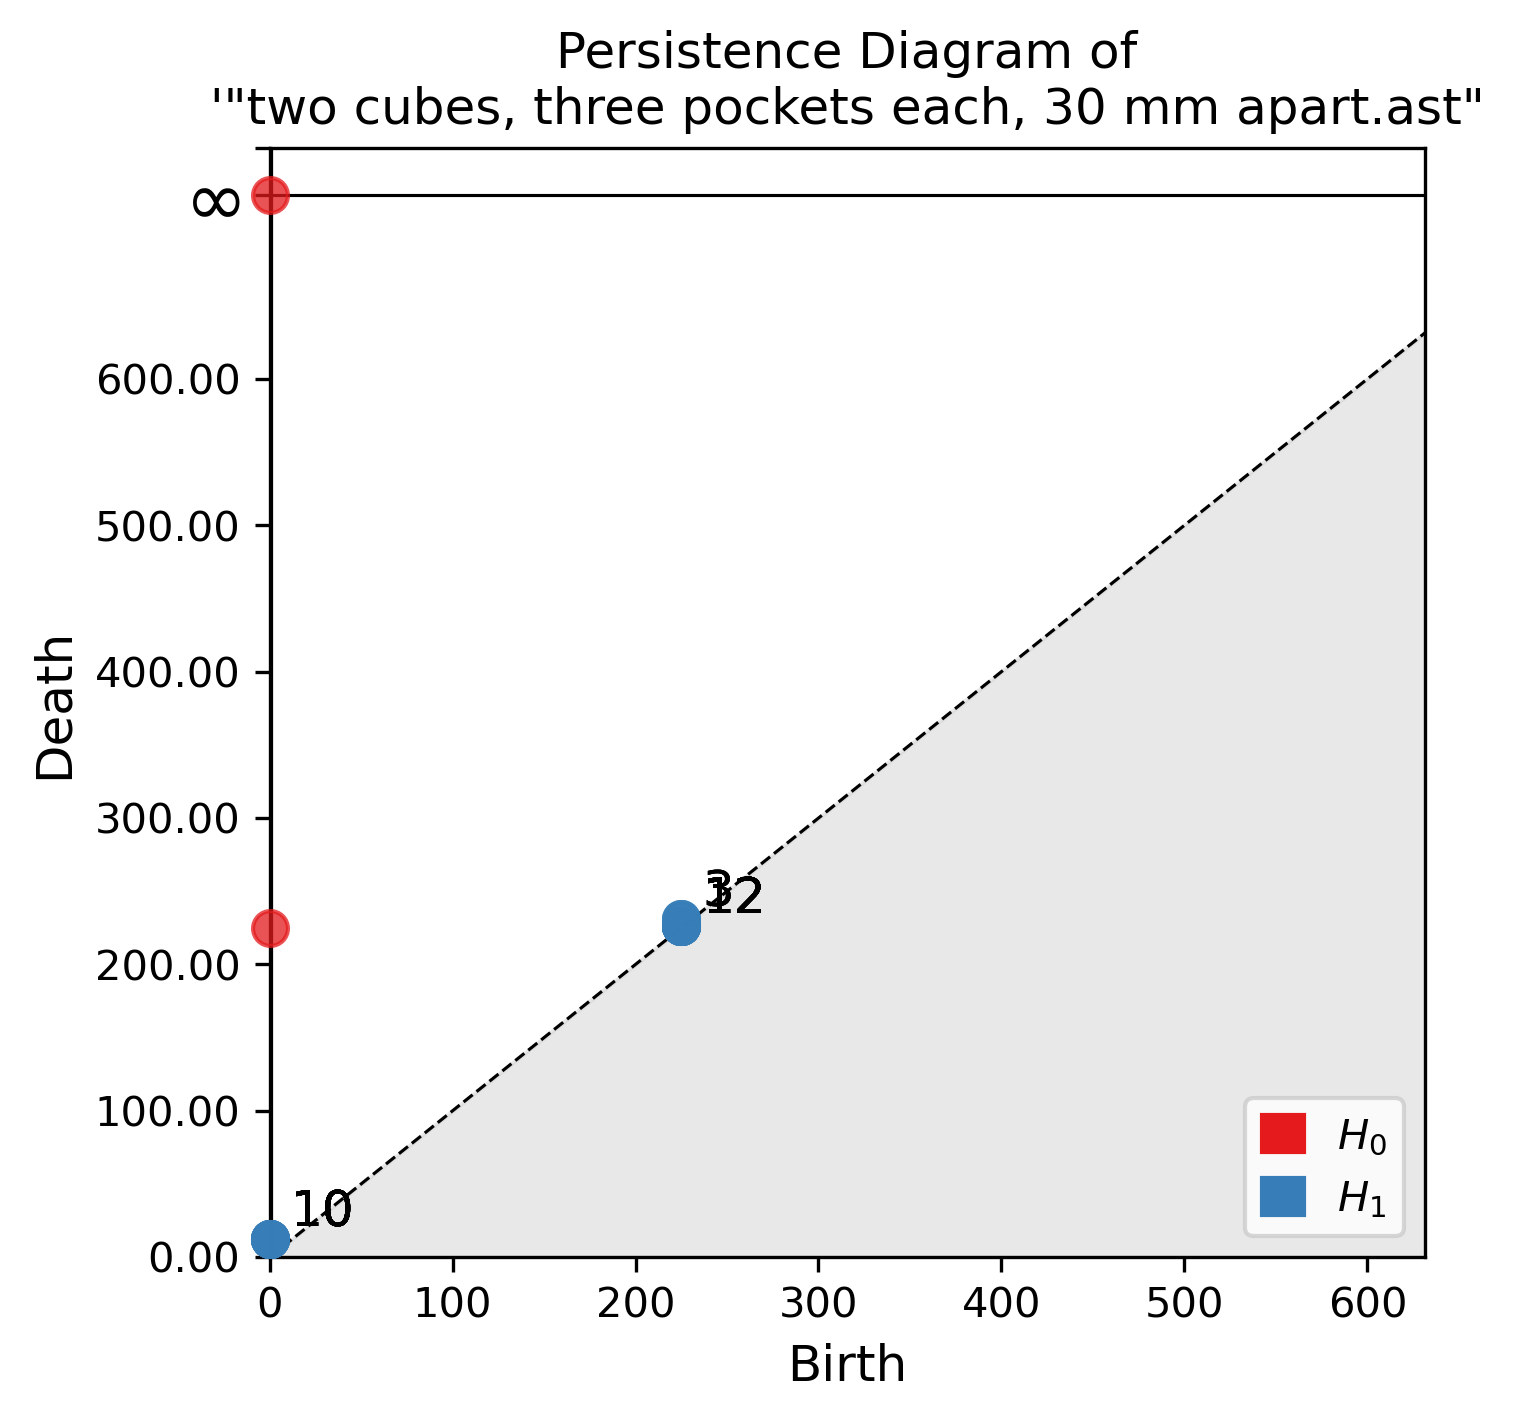
\includegraphics[width=2.5in]{Final Run, (two cubes, three pockets each, 30 mm apart) persdia.png} &
         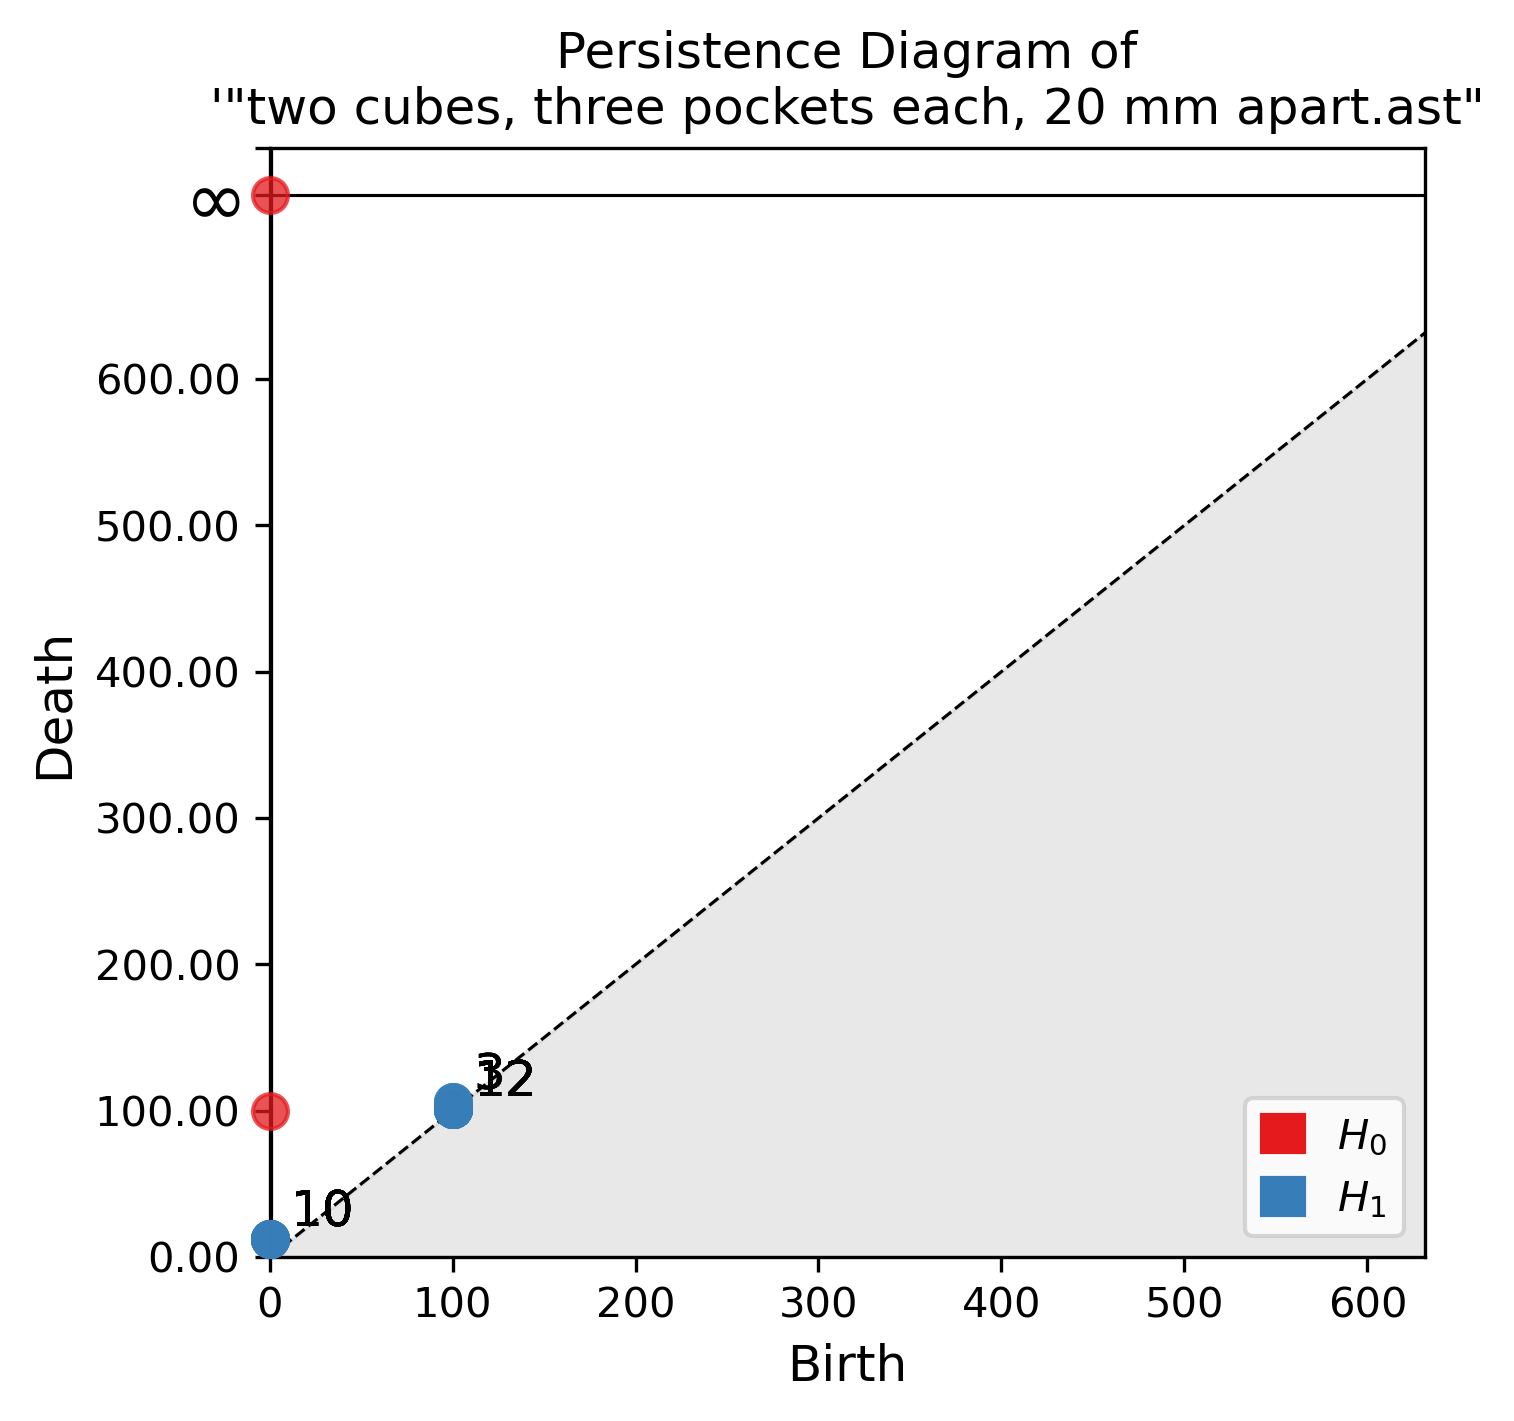
\includegraphics[width=2.5in]{Final Run, (two cubes, three pockets each, 20 mm apart) persdia.png} \\ 
         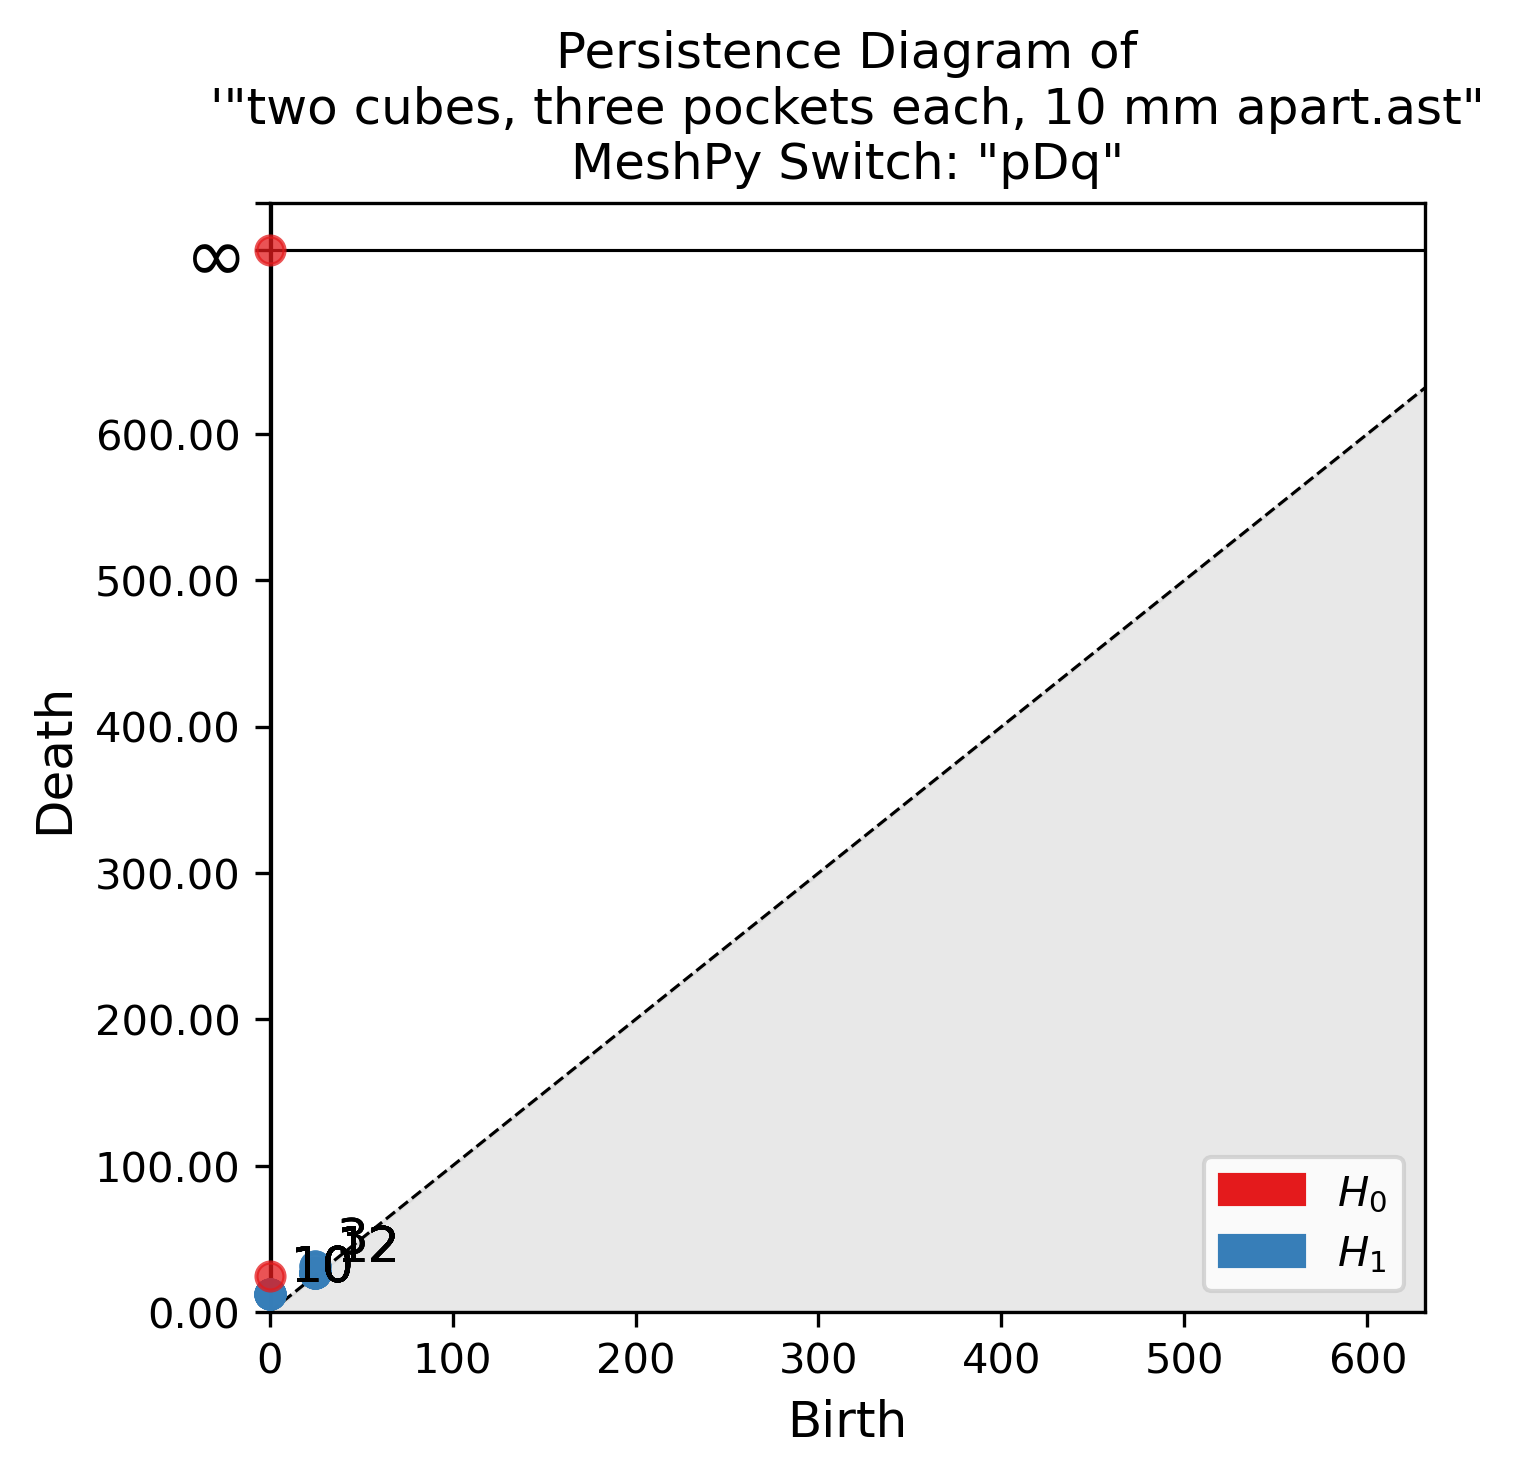
\includegraphics[width=2.5in]{Final Run, (two cubes, three pockets each, 10 mm apart) persdia.png} & 
         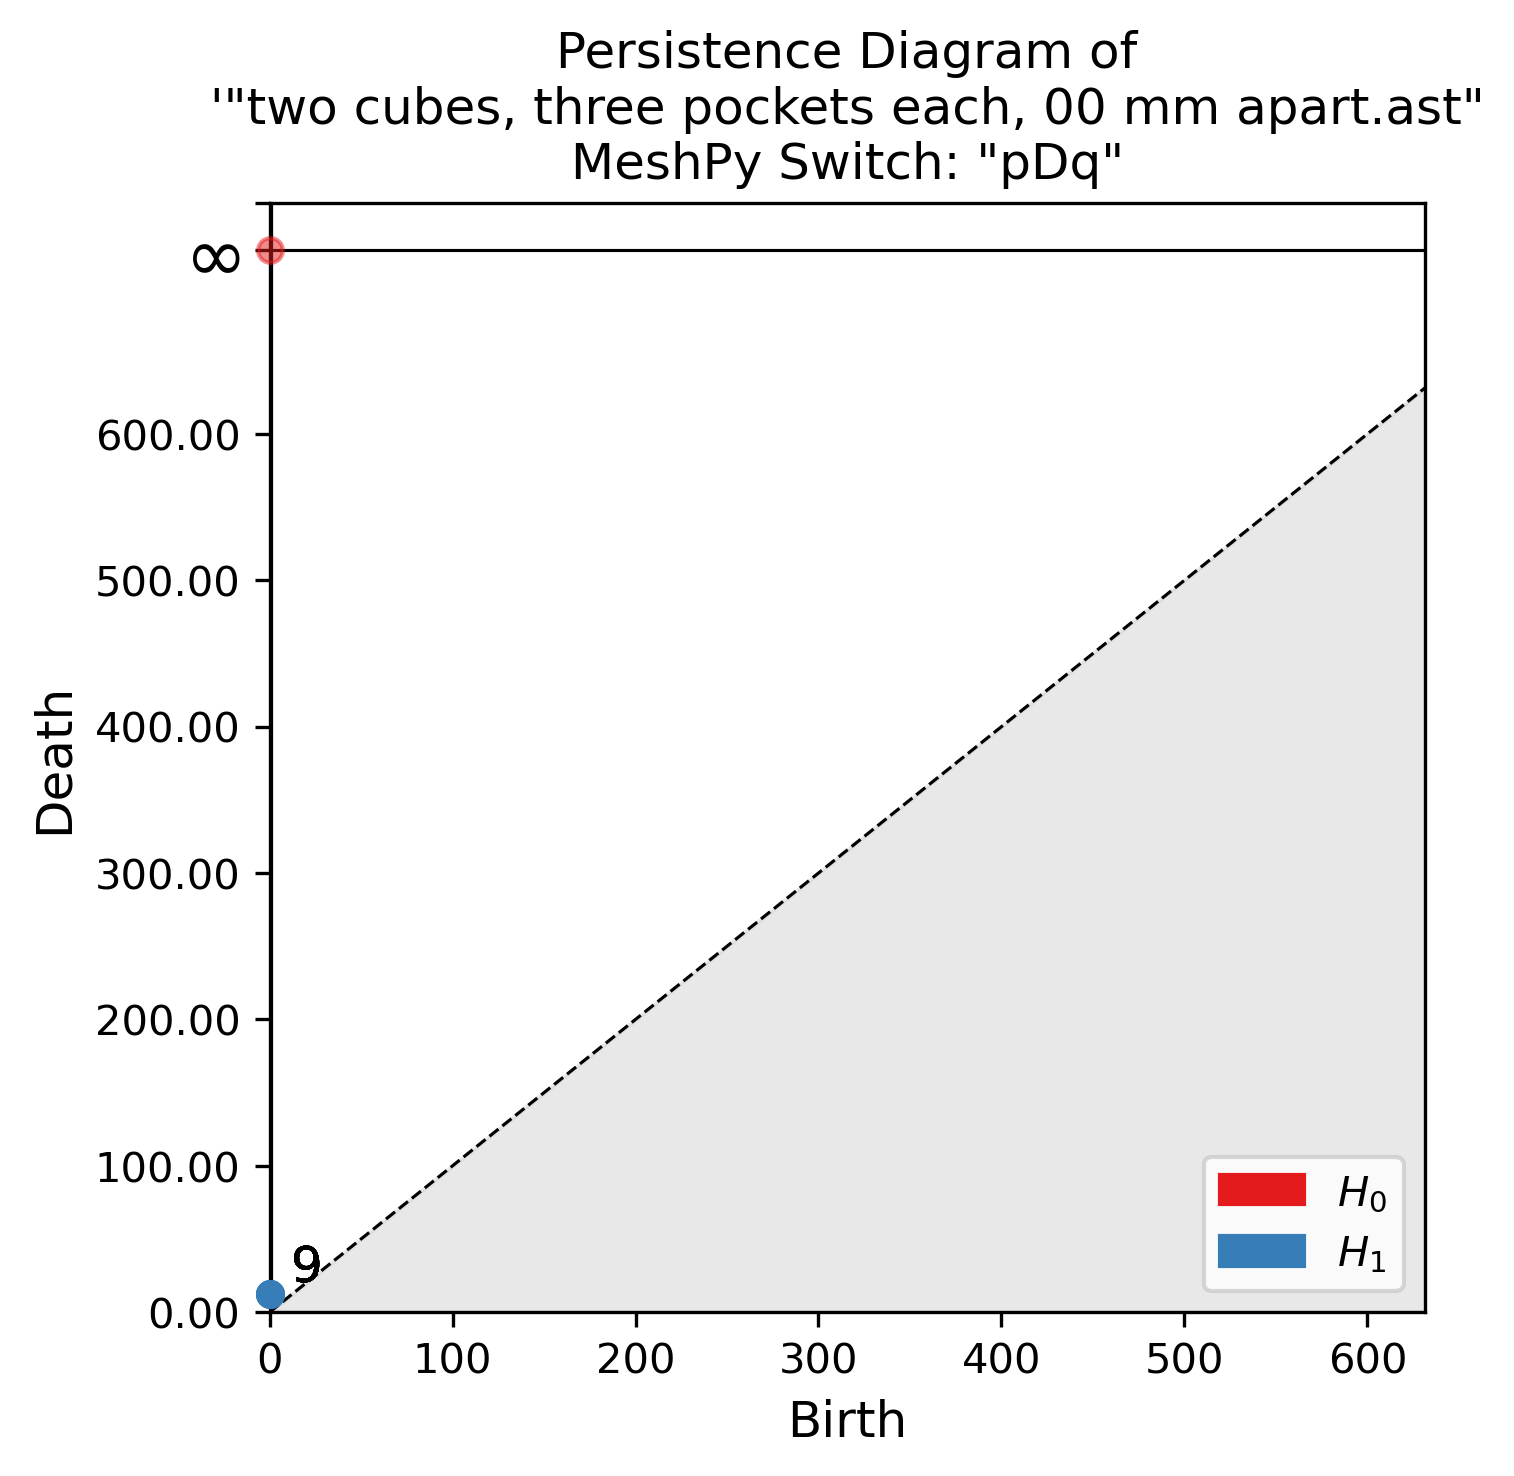
\includegraphics[width=2.5in]{Final Run, (two cubes, three pockets each, 00 mm apart) persdia.png} \\
\end{tabular}
\end{center}
    \caption{Persistence Diagrams of two cubes with three CAD pocket operations that move closer together until combining.}
    \label{fig:cube_two_cubes_persdia_table}
\end{figure}

\newpage
\section{Cube with Equilateral Triangle Hole}
\label{sec:cube_tri_hole}
An equilateral triangle was sketched onto the top face of a cube and a pocket operation was done through the cube. The equilateral triangle hole starts with an edge length of 8mm until it shrinks completely and dissapears.
\begin{figure}[H]
	\begin{center}
    \begin{tabular}{|c|c|c|}
    	 \toprule
         \tstack{\includegraphics[width=1.75in]{Final Run, (cube - equilateral triangle hole 8 mm) MeshPy plotly screenshot.png}\\ {\fontsize{10}{12}\selectfont Equilateral Triangle Hole, 8 mm}} &
         \tstack{\includegraphics[width=1.75in]{Final Run, (cube - equilateral triangle hole 7 mm) MeshPy plotly screenshot.png}\\ {\fontsize{10}{12}\selectfont Equilateral Triangle Hole, 7 mm}} &  
         \tstack{\includegraphics[width=1.75in]{Final Run, (cube - equilateral triangle hole 6 mm) MeshPy plotly screenshot.png}\\ {\fontsize{10}{12}\selectfont Equilateral Triangle Hole, 6 mm}} \\
         \midrule
         \tstack{\includegraphics[width=1.75in]{Final Run, (cube - equilateral triangle hole 5 mm) MeshPy plotly screenshot.png}\\ {\fontsize{10}{12}\selectfont Equilateral Triangle Hole, 5 mm}} & 
         \tstack{\includegraphics[width=1.75in]{Final Run, (cube - equilateral triangle hole 4 mm) MeshPy plotly screenshot.png}\\ {\fontsize{10}{12}\selectfont Equilateral Triangle Hole, 4 mm}} & 
         \tstack{\includegraphics[width=1.75in]{Final Run, (cube - equilateral triangle hole 3 mm) MeshPy plotly screenshot.png}\\ {\fontsize{10}{12}\selectfont Equilateral Triangle Hole, 3 mm}} \\
         \midrule
         \tstack{\includegraphics[width=1.75in]{Final Run, (cube - equilateral triangle hole 2 mm) MeshPy plotly screenshot.png}\\ {\fontsize{10}{12}\selectfont Equilateral Triangle Hole, 2 mm}} & 
         \tstack{\includegraphics[width=1.75in]{Final Run, (cube - equilateral triangle hole 1 mm) MeshPy plotly screenshot.png}\\ {\fontsize{10}{12}\selectfont Equilateral Triangle Hole, 1 mm}} & 
         \tstack{\includegraphics[width=1.75in]{Final Run, (cube - equilateral triangle hole 0 mm) MeshPy plotly screenshot.png}\\ {\fontsize{10}{12}\selectfont Equilateral Triangle Hole, 0 mm}} \\
         \bottomrule
    \end{tabular}
    \end{center}
    \caption{MeshPy plots displayed with Plotly of a cube with an equilateral triangle hole that decreases in size to the original shape.}
    \label{fig:cube_triangle_hole_MeshPy_table}
\end{figure}

\begin{figure}[H]
\begin{center}
    \begin{tabular}{ccc}
         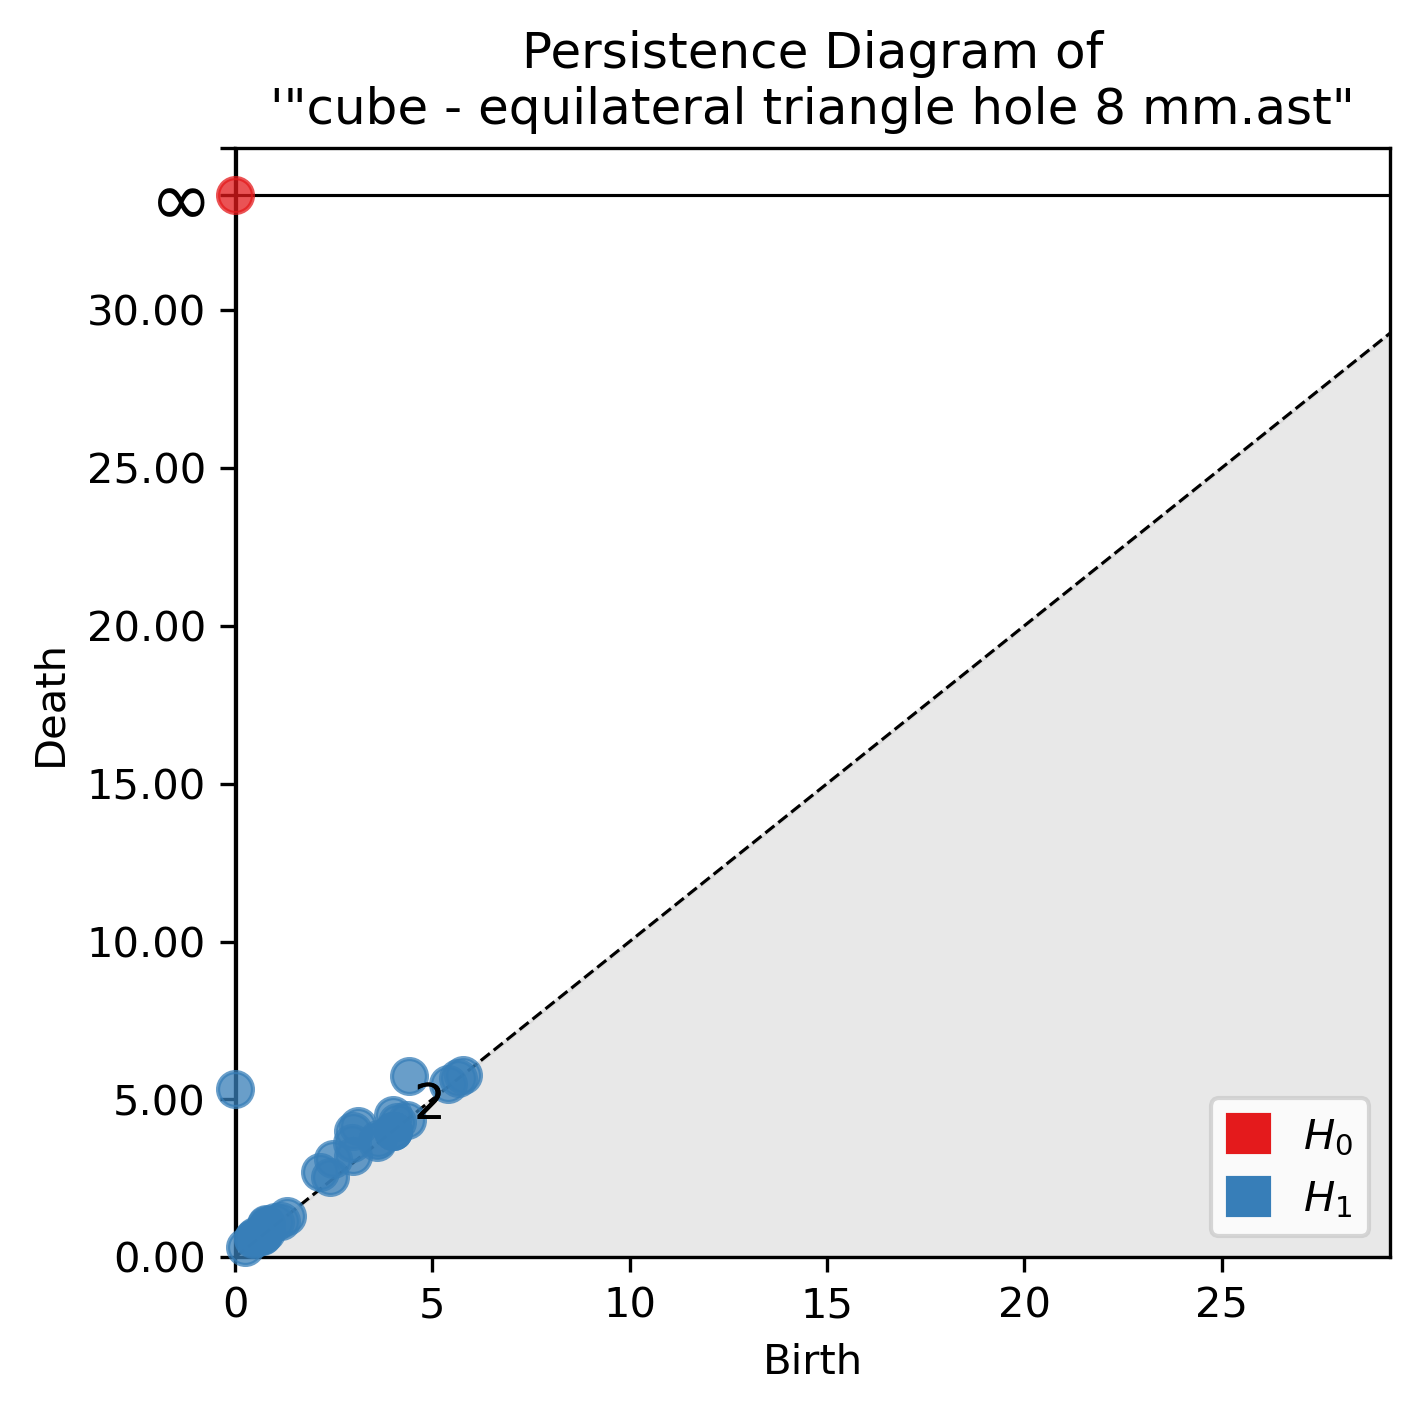
\includegraphics[width=1.875in]{Final Run, (cube - equilateral triangle hole 8 mm) persdia.png} &
         \includegraphics[width=1.875in]{Final Run, (cube - equilateral triangle hole 7 mm) persdia.png} &  
         \includegraphics[width=1.875in]{Final Run, (cube - equilateral triangle hole 6 mm) persdia.png} \\
         \includegraphics[width=1.875in]{Final Run, (cube - equilateral triangle hole 5 mm) persdia.png} & 
         \includegraphics[width=1.875in]{Final Run, (cube - equilateral triangle hole 4 mm) persdia.png} & 
         \includegraphics[width=1.875in]{Final Run, (cube - equilateral triangle hole 3 mm) persdia.png} \\
         \includegraphics[width=1.875in]{Final Run, (cube - equilateral triangle hole 2 mm) persdia.png} & 
         \includegraphics[width=1.875in]{Final Run, (cube - equilateral triangle hole 1 mm) persdia.png} & 
         \includegraphics[width=1.875in]{Final Run, (cube - equilateral triangle hole 0 mm) persdia.png} \\
    \end{tabular}
    \end{center}
    \caption{Persistence Diagrams of a cube with an equilateral triangle hole that decreases in size to the original shape.}
    \label{fig:cube_triangle_hole_persdia_table}
\end{figure}

\newpage
\section{Rectangular Prism Ring with Cut}
\label{sec:rect_prism_ring}
A rectangular prism ring was created as a topologically equivalent model of a solid torus. This was done to allow for faster compute times from a simpler triangulation with less facets. The initial state of the object has a 40mm cut which shrinks and dissapears.
\begin{figure}[H]
\begin{center}
    \begin{tabular}{cccc}
    \toprule
         \tstack{\includegraphics[width=1.4in]{Final Run, (rect prism ring 40 mm cut) MeshPy plotly screenshot.png}\\ {\fontsize{10}{12}\selectfont 40 mm cut}} &
         \tstack{\includegraphics[width=1.4in]{Final Run, (rect prism ring 35 mm cut) MeshPy plotly screenshot.png}\\ {\fontsize{10}{12}\selectfont 35 mm cut}} &
         \tstack{\includegraphics[width=1.4in]{Final Run, (rect prism ring 30 mm cut) MeshPy plotly screenshot.png}\\ {\fontsize{10}{12}\selectfont 30 mm cut}} &
         \tstack{\includegraphics[width=1.4in]{Final Run, (rect prism ring 25 mm cut) MeshPy plotly screenshot.png}\\ {\fontsize{10}{12}\selectfont 25 mm cut}} \\ 
    \midrule
         \tstack{\includegraphics[width=1.4in]{Final Run, (rect prism ring 20 mm cut) MeshPy plotly screenshot.png}\\ {\fontsize{10}{12}\selectfont 20 mm cut}} & 
         \tstack{\includegraphics[width=1.4in]{Final Run, (rect prism ring 15 mm cut) MeshPy plotly screenshot.png}\\ {\fontsize{10}{12}\selectfont 15 mm cut}} &
         \tstack{\includegraphics[width=1.4in]{Final Run, (rect prism ring 10 mm cut) MeshPy plotly screenshot.png}\\ {\fontsize{10}{12}\selectfont 10 mm cut}} & 
         \tstack{\includegraphics[width=1.4in]{Final Run, (rect prism ring 05 mm cut) MeshPy plotly screenshot.png}\\ {\fontsize{10}{12}\selectfont 05 mm cut}} \\ 
    \midrule
         \tstack{\includegraphics[width=1.4in]{Final Run, (rect prism ring 03 mm cut) MeshPy plotly screenshot.png}\\ {\fontsize{10}{12}\selectfont 03 mm cut}} &
         \tstack{\includegraphics[width=1.4in]{Final Run, (rect prism ring 02 mm cut) MeshPy plotly screenshot.png}\\ {\fontsize{10}{12}\selectfont 02 mm cut}} &
         \tstack{\includegraphics[width=1.4in]{Final Run, (rect prism ring 01 mm cut) MeshPy plotly screenshot.png}\\ {\fontsize{10}{12}\selectfont 01 mm cut}} &
         \tstack{\includegraphics[width=1.4in]{Final Run, (rect prism ring 00 mm cut) MeshPy plotly screenshot.png}\\ {\fontsize{10}{12}\selectfont 00 mm cut}} \\
    \bottomrule
    \end{tabular}
    \end{center}
    \caption{MeshPy plots displayed with Plotly of a rectangular prism ring with a cut that decreases to the original shape.}
    \label{fig:rect_prism_ring_MeshPy_table}
\end{figure}

\begin{figure}[H]
\begin{center}
    \begin{tabular}{cccc}
         \includegraphics[width=0.245\textwidth]{Final Run, (rect prism ring 40 mm cut) persdia.png} &
         \includegraphics[width=0.245\textwidth]{Final Run, (rect prism ring 35 mm cut) persdia.png} &  
         \includegraphics[width=0.245\textwidth]{Final Run, (rect prism ring 30 mm cut) persdia.png} &
         \includegraphics[width=0.245\textwidth]{Final Run, (rect prism ring 25 mm cut) persdia.png} \\ 
         \includegraphics[width=0.245\textwidth]{Final Run, (rect prism ring 20 mm cut) persdia.png} & 
         \includegraphics[width=0.245\textwidth]{Final Run, (rect prism ring 15 mm cut) persdia.png} &
         \includegraphics[width=0.245\textwidth]{Final Run, (rect prism ring 10 mm cut) persdia.png} & 
         \includegraphics[width=0.245\textwidth]{Final Run, (rect prism ring 05 mm cut) persdia.png} \\ 
         \includegraphics[width=0.245\textwidth]{Final Run, (rect prism ring 03 mm cut) persdia.png} &
         \includegraphics[width=0.245\textwidth]{Final Run, (rect prism ring 02 mm cut) persdia.png} &
         \includegraphics[width=0.245\textwidth]{Final Run, (rect prism ring 01 mm cut) persdia.png} &
         \includegraphics[width=0.245\textwidth]{Final Run, (rect prism ring 00 mm cut) persdia.png} \\
    \end{tabular}
    \end{center}
    \caption{Persistence Diagrams of a rectangular prism ring with a cut that decreases to the original shape.}
    \label{fig:rect_prism_ring_persdia_table}
\end{figure}

\chapter{Discussion}
\label{chap:discussion}
\section{Two Cubes with Three Pockets Moving Closer}
\label{sec:two_cubes_discussion}
\par Section \ref{sec:two_cubes} features a test case of two cubes with three pocket operations on three orthogonal faces. The cubes move closer together until combining to form one object, as shown in Fig \ref{fig:cube_two_cubes_MeshPy_table}. The three pocket operations on the cube may appear to create 6 holes, but similar to how a non-filled-in tetrahedron has three holes, each cube only has five holes. This can be seen in the figure below of topologically equivalent graphs for a tetrahedron and the cube with three pocket operations (or a non-filled-in cube).
\begin{figure}[H]
    \centering
    \begin{subfigure}[b]{0.3\textwidth}
        \centering
        \includegraphics[width=\textwidth]{networkx_tetra.png}
    \end{subfigure}
    \begin{subfigure}[b]{0.3\textwidth}
        \centering
        \includegraphics[width=\textwidth]{networkx_cube.png}
    \end{subfigure}
    \caption{Network graphs of a non-filled-in tetrahedron and cube.}
\end{figure}
\par The decreasing distance between the objects and the change in topology which occurs when the objects combine are represented in Fig \ref{fig:cube_two_cubes_persdia_table} as a sequence of persistence diagrams. Initially the two cubes appear as two connected components in $H_{0}$ with birth-death points at (0, 625) and (0, $\infty$). One connected component dies at $r^{2} = 625$. This is equivalent to a Euclidean distance of $r=25$mm which means the open balls of each connected component intersect at the halfway point of the distance, 50mm, between each object. The other connected component was chosen by \verb"Gudhi" to be the first point in the complex, so it does not die and has a death time of $r^2=\infty$. As the two cubes move closer together, we can convert their distance apart to an $H_{0}$ death time by taking the square of their circumradius, which in this case is the shortest distance of two vertices between the two inward faces of each cube: $\mathsf{Death}=(\frac{\mathsf{Dist}}{2})^2$. Conversly, the $H_{0}$ death time of a cube can be used to find the distance between two cubes: $\mathsf{Dist} = 2\sqrt{\mathsf{Death}}$. This also explains the value for the death times of $H_{1}$ points that represent the holes of the cubes. Each hole is a 5mm square and has a death time of $r^{2}=12.5$. This is equivalent to $r^{2}=(\frac{5\sqrt{2}}{2})^{2}$, where $5\sqrt{2}$ is the distance of the diagonal of the squares. The additional $H_{1}$ points on the diagonal are noise and appear when the open balls of vertices between the two inward faces of each cube intersect.
\begin{table}[H]
\centering
\begin{tabular}{|c|c|}
    \hline
    \makecell{Distance\\(mm)} & \makecell{Connected\\Component\\Death Time} \\
    \hline
    50 & 625 \\
    40 & 400 \\
    30 & 225 \\
    20 & 100 \\
    10 & 25 \\
    0 & $\infty$ \\
    \hline
\end{tabular}
\caption{Distances between cubes and the corresponding $H_{0}$ death times.}
\label{tab:two_cubes_death_times}
\end{table}

\par In Table \ref{tab:two_cubes_death_times}, as the distance shrinks between the two cubes, we can see the death time of the second connected component move closer to 0. When the two cubes combine, there is only one point in $H_{0}$ with a death time of $\infty$ because there is only one connected component. The merger of cubes also shows one of the holes no longer exists as there are 9 $H_{1}$ points instead of 10.
\par In terms of tolerancing between two 3D parts, we can use the base formulas of $d=r^{2}$ and $r=\sqrt{d}$, where $r$ is euclidean radius and $d$ is death time, along with intuition about how to choose the radii for the formula (set radius equal to half the distance apart in this case) to determine which death time would create the optimal tolerance in fabrication and vice versa. For example, if a fabrication method such as 3D printing had a tolerance of 3mm (this is a realistic tolerance for large-scale printers which print car prototyping parts), we can use $d=(\mathsf{\frac{3}{2}})^{2}$ to find that the $H_{0}$ death time of a part feature would need to have a have a margin of error of $\pm 2.25$ to ensure a good fit with other part features in close proximity to it.
\newpage
\section{Cube with Equilateral Triangle Hole}
\label{sec:eq_tri_hole}
\par Section \ref{sec:cube_tri_hole} features a test case of a cube with a pocket of an equilateral triangle through the entire object, creating an equilateral triangle hole. The equilateral triangle hole begins with an edge length of 8mm and decreases in length until the hole dissapears. As expected, there is only one connected component as a point in $H_{0}$ with a death time of $\infty$.
\par Unfortunately, the nature of how the new refined Delauanay triangulation mesh was generated from the original STL mesh caused problems with the results. The errors between hole death times in Table \ref{tab:eq_tri_hole_table} is a result of miscalculations due to the fineness of the mesh generated by \verb"MeshPy". To understand the reasons why the errors occurred, we will use the formula to find the circumradius of an equilateral triangle: 
$$r = \frac{l}{\sqrt{3}}\text{, where }l\text{ is the edge length.}$$

We will also use the radius of a triangle's inscribed circle. The inscribed circle of an equilateral triangle exists within the triangle and is tangent to each edge in the triangle. The formula to find the inscribed radius is the following:
$$r = \frac{l}{2\sqrt{3}}\text{, where }l\text{ is the edge length.}$$

\begin{table}[H]
\centering
\begin{tabular}{|c|c|c|c|c|c|c|}
    \hline
    \makecell{Edge\\Length\\(mm)} & \makecell{Circum-\\radius\\(mm), $r_{c}$} & \makecell{Inscribed\\ radius\\ (mm), $r_{i}$} & \makecell{$d=r_{c}^{2}$\\Death\\Time} & \makecell{$d=r_{i}^{2}$\\Death\\Time} & \makecell{Figure \ref{fig:cube_triangle_hole_persdia_table}\\$H_1$ Death\\ Time} & \makecell{Original STL\\$H_{1}$ Death\\Time}\\
    \hline
    8     & 4.619 & 2.309 & 21.$\overline{333}$ & $5.\overline{333}$ & $5.\overline{333}$ & 21.$\overline{333}$\\
    7     & 4.041 & 2.021 & 16.$\overline{333}$ & $4.08\overline{3}$ & 4.567 & 16.$\overline{333}$\\
    6     & 3.464 & 1.732 & 12.000 & 3.000 & 9.000 & 12.000\\
    5     & 2.887 & 1.443 & 8.$\overline{333}$ & $2.08\overline{3}$ & $8.\overline{333}$ & 8.$\overline{333}$\\
    4     & 2.309 & 1.155 & $5.\overline{333}$ & $1.\overline{333}$ & $5.\overline{333}$ & $5.\overline{333}$\\
    3     & 1.732 & 0.866 & 3.000 & 0.750 & $2.\overline{999}$ & $2.\overline{999}$\\
    2     & 1.155 & 0.577 & $1.\overline{333}$ & $0.\overline{333}$ & $1.\overline{333}$ & $1.\overline{333}$\\
    1     & 0.577 & 0.289 & $0.\overline{333}$ & $0.08\overline{3}$ & $0.\overline{333}$ & $0.\overline{333}$\\
    \hline
\end{tabular}
\cprotect\caption{Equilateral triangle hole edge lengths and their corresponding death time comparisons between predictions calculated from triangle circumradius and inradius with observed death times from the \verb"MeshPy" Delaunay triangulation mesh and the original STL file mesh.}
\label{tab:eq_tri_hole_table}
\end{table}
\par The death times of an equilateral triangle is expected to be found from using the square of the circumradius, $r_{c}$, as the Delaunay triangulation ensures the vertices of triangles created in the new mesh are all self-contained on the surface boundary of their respective circumspheres. This means that the expanding circumcircles from each vertex in the plane of an equilateral triangle will meet at the intersection of the three perpendicular bisectors of each triangle edge, and the radius of these circumcircles at the intersection will be equal to the the radius of the triangle's circumsphere. Thus, taking the square of $r_{c}$ will give us the death time of this triangle if it is not "filled-in".
\par The column of $H_{1}$ death times from persistence diagrams in Fig \ref{fig:cube_triangle_hole_persdia_table} shows the death times for edge lengths 5mm through 1mm all match the death times calculated with $r_{c}$. We can see the reason for this correlation in the sequence of meshes created with \verb"MeshPy" in Fig \ref{fig:cube_triangle_hole_MeshPy_table}: meshes for edge lengths 5mm through 1mm all consist of only three points to create the triangle.
\par However, for edge lengths 8mm through 6mm, the \verb"MeshPy" switch \verb"-q" caused the mesh to include many new points in close proximity to each other due to the relatively smaller distances between the vertices of the triangle hole and the edges of the top and bottom faces of the cube. The additional points were also added to the triangle hole edges for these lengths, which caused the Alpha complex to form a hole sooner in $r^{2}$ with smaller open metric balls due to the triangles containing more than the minimum three points. This results in the death times of the $H_{1}$ points being much smaller than the calculated death time with $r_{c}$.
\par The death times from Fig \ref{fig:cube_triangle_hole_persdia_table} for edge lengths ranging 8mm through 6mm all either match the death times calculated from the inscribed radius $r_{i}$ (8mm), are close to the death times from $r_{i}$ (7mm), or are in between the death times from $r_{i}$ or $r_{c}$ (6mm and 7mm). The square of the inscribed radius is the lower bound of possible radii to compute the death time of an equilateral triangle. This is becuase it is possible for the smallest  distance from points on an equilateral triangle edge to the intersection points of perpendicular bisectors of its three edges to be the distance from the midpoint to that intersection point, or $\frac{l}{2\sqrt{3}}$. Therefore the lower bound death time for an equilateral triangle is $r^{2}=(\frac{l}{2\sqrt{3}})^{2}$.
\par In most cases, more points need to be added to the mesh in order to make the original STL mesh a Delaunay triangulation. However, as we have seen this can create errors in generating the persistence points in $H_{1}$. Table \ref{tab:eq_tri_hole_table} also shows the death times of triangle holes using the original STL mesh as the input for the Alpha complex. In cases such as these, the desired feature of analysis, the triangle hole, is already a Delaunay triangulation, so increasing the fineness of the mesh through \verb"MeshPy" is not necessary because the death times of the ASCII STL mesh all match (taking into account possible floating-point error) the death times calculated with $r_{c}$.

\newpage
\section{Rectangular Prism Ring with Cut}
\par Section \ref{sec:rect_prism_ring} features a rectangular prism ring, meant to be a simplified model of a solid torus, which has a portion cut out of it. The cut starts at 40mm wide and decreases in length until the cut dissappears to the final shape of a ring.
\par The three $H_{1}$ points of holes slightly above the diagonal can be considered noise for the same reason as the noise in Fig \ref{fig:cube_two_cubes_persdia_table} as we discussed in Section \ref{sec:two_cubes_discussion}. However, the $H_{1}$ point which is not noise represents the time it takes for the hole to form once the gap of open metric balls in the Alpha complex intersect.
\begin{table}[H]
\centering
\begin{tabular}{|c|c|c|}
    \hline
    \makecell{Length of\\Cut (mm)} & Birth Time & Death Time \\
    \hline
    40 & 400.0000 & 500.0000 \\
    35 & 306.2500 & 425.0000 \\
    30 & 225.0000 & 431.6406 \\
    25 & 156.2500 & 415.2588 \\
    20 & 100.0000 & 406.2500 \\
    15 & 56.2500 & 401.9775 \\
    10 & 25.0000 & 400.3906 \\
    5 & 6.2500 & 400.0244 \\
    3 & 2.2500 & 400.0032 \\
    2 & 1.0000 & 400.0006 \\
    1 & 0.2500 & 400.0001 \\
    0 & 0.0000 & 400.0000 \\
    \hline
\end{tabular}
\caption{Cut lengths and the birth and death times of holes, from Fig \ref{fig:rect_prism_ring_persdia_table}.}
\end{table}
\par The birth times of the holes are formed through the same type of motion as in Section \ref{sec:two_cubes_discussion} where two features move closer together until combining. This causes the birth times to follow the same pattern of $\mathsf{Dist} = 2\sqrt{\mathsf{Death}}$. Aside from the cut length of 30mm, the death times also follow a pattern of decreasing from 500 to converge to 400. The death times converge to 400 because the width of the square hole in the rectangular prism ring is 40mm, so we can calculate that 400 should be the death time by $\mathsf{Death}=(\frac{\mathsf{Dist}}{2})^2$.
\par While the birth time or death time could be used for choosing a tolerance or clearance value for a part's design, it would be easier to choose these values based on birth time. The death times also correspond to the length of the cuts, but in order to choose a tolerance value closer to 0.5mm or lower, floating-point errors could begin to be a problem with the difference between death time and $r^{2} = 400$.
\chapter{Conclusion}

\section{Findings}\par In this paper we outlined a method for analyzing 3D ASCII STL files to determine metrics for when a feature of a part may have a margin of error in its tolerance or clearance which could cause issues in fabrication. We first pass in the STL data to \verb"MeshPy" to generate a Delaunay triangulation of the surface of the object. This is done to ensure features of parts are accurately represented in $H_{0}$ and $H_{1}$ by the Alpha complex filtered simplices. However, depending on the part feature to be analyzed, meshing can cause errors to occur (see Sec \ref{sec:eq_tri_hole}). We then compare the simplices of the Alpha complex to the simplices of the Delaunay triangulation mesh to assign a birth time of 0 to the Alpha complex simplices which were originally in the Delaunay triangulation mesh. Using these modified persistence point values, we visualize the persitent homology of a part with a Persistence Diagram. We then repeat these steps for a sequence of variations of altered part feature measurements as separate STL files to determine potential patterns in the birth and death times of the feature.

\section{Future Work}
\par For computational efficiency, the implementation could be improved by checking if the mesh originally contained within a 3D object file is Delaunay or not upon parsing to determine if it is necessary to create a new mesh with meshpy. Potentially eliminating this step would reduce the overall computational expense of the program.
\par The variations of the three cases of 3D objects were created manually in FreeCAD, but creating the variations could be automated. This can happen either through using the FreeCAD python library and editing the original FreeCAD .FCStd file or or by editing the text of the exported ASCII STL file to manipulate facets and vertices to change part features to simulate different tolerances.
\par The methods of this paper can be improved upon by computing a measure of topological stability to determine the error from the "truth" of an STL file through analyzing the different persistence diagrams of the different versions of the file. The "truth" value of the 3D object would be the persistence vector of the preselected object and the error would be computed through the differences in the persistence vectors of the variations.
\par This paper only analyzes connected components and holes. When the \verb"MeshPy" meshes of 3D objects were created, it only triangulated the outer surfaces of objects. So when an object with a void was given to the program, it created a mesh of only the outer surface and inner surface of the void, but did not tetrahedralize the space between the two surfaces. This led to voids having a birth time not equal to $r^{2}=0$ because the voids were born as balls grew throughout the progression of the Alpha complex. The methods of this paper can also be improved through finding the correct meshing algorithm to tetrahedralize the space between surfaces in an object containing a void, as well as fully enclosed objects.

\bibliography{thesis_bib}
\bibliographystyle{plain}
\backmatter
\end{document}
